\documentclass[a4paper,10pt]{article} % {{{
\usepackage{listings,amssymb,amsmath,amsthm,graphicx,float,hyperref,wrapfig,subfig}

\hypersetup{
    colorlinks=false,
    pdfborder={0 0 0},
}

\newcommand{\tsup}[1]{\ensuremath{
    \sp{\text{#1}}
}}

% Template coming from Pygments (pygmentize with "-O full,preamble")

\usepackage{fancyvrb}
\usepackage{color}

\makeatletter
\def\PY@reset{\let\PY@it=\relax \let\PY@bf=\relax%
    \let\PY@ul=\relax \let\PY@tc=\relax%
    \let\PY@bc=\relax \let\PY@ff=\relax}
\def\PY@tok#1{\csname PY@tok@#1\endcsname}
\def\PY@toks#1+{\ifx\relax#1\empty\else%
    \PY@tok{#1}\expandafter\PY@toks\fi}
\def\PY@do#1{\PY@bc{\PY@tc{\PY@ul{%
    \PY@it{\PY@bf{\PY@ff{#1}}}}}}}
\def\PY#1#2{\PY@reset\PY@toks#1+\relax+\PY@do{#2}}

\def\PY@tok@gd{\def\PY@tc##1{\textcolor[rgb]{0.63,0.00,0.00}{##1}}}
\def\PY@tok@gu{\let\PY@bf=\textbf\def\PY@tc##1{\textcolor[rgb]{0.50,0.00,0.50}{##1}}}
\def\PY@tok@gt{\def\PY@tc##1{\textcolor[rgb]{0.00,0.25,0.82}{##1}}}
\def\PY@tok@gs{\let\PY@bf=\textbf}
\def\PY@tok@gr{\def\PY@tc##1{\textcolor[rgb]{1.00,0.00,0.00}{##1}}}
\def\PY@tok@cm{\def\PY@tc##1{\textcolor[rgb]{0.50,0.50,0.50}{##1}}}
\def\PY@tok@vg{\let\PY@bf=\textbf\def\PY@tc##1{\textcolor[rgb]{0.82,0.44,0.00}{##1}}}
\def\PY@tok@m{\let\PY@bf=\textbf\def\PY@tc##1{\textcolor[rgb]{0.38,0.00,0.88}{##1}}}
\def\PY@tok@mh{\let\PY@bf=\textbf\def\PY@tc##1{\textcolor[rgb]{0.00,0.31,0.50}{##1}}}
\def\PY@tok@cs{\let\PY@bf=\textbf\def\PY@tc##1{\textcolor[rgb]{0.80,0.00,0.00}{##1}}}
\def\PY@tok@ge{\let\PY@it=\textit}
\def\PY@tok@vc{\def\PY@tc##1{\textcolor[rgb]{0.19,0.38,0.56}{##1}}}
\def\PY@tok@il{\let\PY@bf=\textbf\def\PY@tc##1{\textcolor[rgb]{0.00,0.00,0.82}{##1}}}
\def\PY@tok@go{\def\PY@tc##1{\textcolor[rgb]{0.50,0.50,0.50}{##1}}}
\def\PY@tok@cp{\def\PY@tc##1{\textcolor[rgb]{0.31,0.44,0.56}{##1}}}
\def\PY@tok@gi{\def\PY@tc##1{\textcolor[rgb]{0.00,0.63,0.00}{##1}}}
\def\PY@tok@gh{\let\PY@bf=\textbf\def\PY@tc##1{\textcolor[rgb]{0.00,0.00,0.50}{##1}}}
\def\PY@tok@ni{\let\PY@bf=\textbf\def\PY@tc##1{\textcolor[rgb]{0.50,0.00,0.00}{##1}}}
\def\PY@tok@nl{\let\PY@bf=\textbf\def\PY@tc##1{\textcolor[rgb]{0.56,0.44,0.00}{##1}}}
\def\PY@tok@nn{\let\PY@bf=\textbf\def\PY@tc##1{\textcolor[rgb]{0.05,0.52,0.71}{##1}}}
\def\PY@tok@no{\let\PY@bf=\textbf\def\PY@tc##1{\textcolor[rgb]{0.00,0.19,0.38}{##1}}}
\def\PY@tok@na{\def\PY@tc##1{\textcolor[rgb]{0.00,0.00,0.75}{##1}}}
\def\PY@tok@nb{\def\PY@tc##1{\textcolor[rgb]{0.00,0.44,0.13}{##1}}}
\def\PY@tok@nc{\let\PY@bf=\textbf\def\PY@tc##1{\textcolor[rgb]{0.69,0.00,0.38}{##1}}}
\def\PY@tok@nd{\let\PY@bf=\textbf\def\PY@tc##1{\textcolor[rgb]{0.31,0.31,0.31}{##1}}}
\def\PY@tok@ne{\let\PY@bf=\textbf\def\PY@tc##1{\textcolor[rgb]{0.94,0.00,0.00}{##1}}}
\def\PY@tok@nf{\let\PY@bf=\textbf\def\PY@tc##1{\textcolor[rgb]{0.00,0.38,0.69}{##1}}}
\def\PY@tok@si{\def\PY@bc##1{\colorbox[rgb]{0.88,0.88,0.88}{##1}}}
\def\PY@tok@s2{\def\PY@bc##1{\colorbox[rgb]{1.00,0.94,0.94}{##1}}}
\def\PY@tok@vi{\def\PY@tc##1{\textcolor[rgb]{0.19,0.19,0.69}{##1}}}
\def\PY@tok@nt{\def\PY@tc##1{\textcolor[rgb]{0.00,0.44,0.00}{##1}}}
\def\PY@tok@nv{\def\PY@tc##1{\textcolor[rgb]{0.56,0.38,0.19}{##1}}}
\def\PY@tok@s1{\def\PY@bc##1{\colorbox[rgb]{1.00,0.94,0.94}{##1}}}
\def\PY@tok@gp{\let\PY@bf=\textbf\def\PY@tc##1{\textcolor[rgb]{0.78,0.36,0.04}{##1}}}
\def\PY@tok@sh{\def\PY@bc##1{\colorbox[rgb]{1.00,0.94,0.94}{##1}}}
\def\PY@tok@ow{\let\PY@bf=\textbf\def\PY@tc##1{\textcolor[rgb]{0.00,0.00,0.00}{##1}}}
\def\PY@tok@sx{\def\PY@tc##1{\textcolor[rgb]{0.82,0.13,0.00}{##1}}
    \def\PY@bc##1{\colorbox[rgb]{1.00,0.94,0.94}{##1}}}
\def\PY@tok@bp{\def\PY@tc##1{\textcolor[rgb]{0.00,0.44,0.13}{##1}}}
\def\PY@tok@c1{\def\PY@tc##1{\textcolor[rgb]{0.50,0.50,0.50}{##1}}}
\def\PY@tok@kc{\let\PY@bf=\textbf\def\PY@tc##1{\textcolor[rgb]{0.00,0.50,0.00}{##1}}}
\def\PY@tok@c{\def\PY@tc##1{\textcolor[rgb]{0.50,0.50,0.50}{##1}}}
\def\PY@tok@mf{\let\PY@bf=\textbf\def\PY@tc##1{\textcolor[rgb]{0.38,0.00,0.88}{##1}}}
\def\PY@tok@err{\def\PY@tc##1{\textcolor[rgb]{0.94,0.00,0.00}{##1}}
    \def\PY@bc##1{\colorbox[rgb]{0.94,0.63,0.63}{##1}}}
\def\PY@tok@kd{\let\PY@bf=\textbf\def\PY@tc##1{\textcolor[rgb]{0.00,0.50,0.00}{##1}}}
\def\PY@tok@ss{\def\PY@tc##1{\textcolor[rgb]{0.63,0.38,0.00}{##1}}}
\def\PY@tok@sr{\def\PY@tc##1{\textcolor[rgb]{0.00,0.00,0.00}{##1}}
    \def\PY@bc##1{\colorbox[rgb]{1.00,0.94,1.00}{##1}}}
\def\PY@tok@mo{\let\PY@bf=\textbf\def\PY@tc##1{\textcolor[rgb]{0.25,0.00,0.88}{##1}}}
\def\PY@tok@mi{\let\PY@bf=\textbf\def\PY@tc##1{\textcolor[rgb]{0.00,0.00,0.82}{##1}}}
\def\PY@tok@kn{\let\PY@bf=\textbf\def\PY@tc##1{\textcolor[rgb]{0.00,0.50,0.00}{##1}}}
\def\PY@tok@o{\def\PY@tc##1{\textcolor[rgb]{0.19,0.19,0.19}{##1}}}
\def\PY@tok@kr{\let\PY@bf=\textbf\def\PY@tc##1{\textcolor[rgb]{0.00,0.50,0.00}{##1}}}
\def\PY@tok@s{\def\PY@bc##1{\colorbox[rgb]{1.00,0.94,0.94}{##1}}}
\def\PY@tok@kp{\let\PY@bf=\textbf\def\PY@tc##1{\textcolor[rgb]{0.00,0.19,0.50}{##1}}}
\def\PY@tok@w{\def\PY@tc##1{\textcolor[rgb]{0.73,0.73,0.73}{##1}}}
\def\PY@tok@kt{\let\PY@bf=\textbf\def\PY@tc##1{\textcolor[rgb]{0.19,0.19,0.56}{##1}}}
\def\PY@tok@sc{\def\PY@tc##1{\textcolor[rgb]{0.00,0.25,0.82}{##1}}}
\def\PY@tok@sb{\def\PY@bc##1{\colorbox[rgb]{1.00,0.94,0.94}{##1}}}
\def\PY@tok@k{\let\PY@bf=\textbf\def\PY@tc##1{\textcolor[rgb]{0.00,0.50,0.00}{##1}}}
\def\PY@tok@se{\let\PY@bf=\textbf\def\PY@tc##1{\textcolor[rgb]{0.38,0.38,0.38}{##1}}
   } % \def\PY@bc##1{\colorbox[rgb]{1.00,0.94,0.94}{##1}}}
\def\PY@tok@sd{\def\PY@tc##1{\textcolor[rgb]{0.82,0.25,0.13}{##1}}}

\def\PYZbs{\char`\\}
\def\PYZus{\char`\_}
\def\PYZob{\char`\{}
\def\PYZcb{\char`\}}
\def\PYZca{\char`\^}
% for compatibility with earlier versions
\def\PYZat{@}
\def\PYZlb{[}
\def\PYZrb{]}
\makeatother



% gebruik '\and' tussen authors, '\\' voor extra info over een author.
\author{Harm Dermois (5027963) \and Joris Stork (6185320) \and
Lucas Swartsenburg (6174388) \and Sander van Veen (6167969)}

\title{Cobots and Sun SPOTs: a robotics project}

% }}}

\begin{document}

\maketitle

% Disable page number of title page
\thispagestyle{empty}

\begin{figure}[H]
\label{fig:cobot_sunspot_final}
\centering
\includegraphics[width=0.95\textwidth]{img/sunspot_cobot_final_together.png}
\caption{Left: Cobot with Sun SPOT attached; right: Sun SPOT for remote control.}
\end{figure}

\abstract{This is our final report for the 2011 robotics project at the
University of Amsterdam. Our goal was to write a C driver for the Jobot; to
create a communications channel between a Jobot and Sun SPOT; and to communicate
wirelessly between multiple Sun SPOT / Jobot pairs. We succeeded with respect to
the first two goals. Our communications implementation includes a deterministic
bit banging protocol that involves error checking and handshaking. Our robot
driver code generates low-level signals to command and coordinate the robot's
servos.  Last, but not least, we composed an efficient toolchain to program our
C driver on the Jobot.}

\pagebreak

\tableofcontents

\pagebreak

\section{Introduction} % {{{

This project concludes our team's involvement in a January 2011 robotics course
at the University of Amsterdam. The team consists of four second-year UvA
students enrolled for the BSc in computer science. The overall aim of this
project has been to address the challenges inherent in programming a
microcontroller based mobile robot and handling communication between multiple,
differing devices as might be required for a typical robotics application.

In this project, our team was given the task, firstly, of ``resuscitating'' the
UvA's Java-programmable ``Jobot'' robots, whose software development platform
had become defunct and inoperative. Our second task was to combine the Jobots'
mobility and sensing capabilities with the enhanced communications, sensing and
processing functionality of Sun SPOTs -- wireless sensor network devices
Developed by Sun Labs. In this way, we hoped to achieve a few things, namely to:

\begin{itemize}
    \item write, compile and load programs from scratch for a PIC based
    microcontroller board;
    \item create drivers for the servos and sensors connected to the board
    mentioned above;
    \item further explore the Sun SPOTs' sensing and communications
    characteristics through those devices' Java frameworks;
    \item build a data communication channel between the Sun SPOTs and the
    standard microcontrollers on the Jobots. Investigate whether this could be
    achieved over an $I^2C$ bus;
    \item design an interface between our respective software implementations on
    the Jobot and on the Sun SPOTs;
    \item build a remote control system using the above interface;
    \item attempt some basic robot activities using our adapted, Sun SPOT
    controlled robot(s), such as: obstacle avoidance; reaching a goal;
    recognising a fellow robot; following a fellow robot, and so on; and
    \item learn to work with embedded chips and low-level signal handling.
\end{itemize}

Strict time and resource limitations took precedence over any adherence
to pre-formulated goals and methods. That said, our project was successful,
and our team achieved a bonus on the way.

This report describes the principal materials at our disposal and our approach
to completing the given project tasks. Our methods are described per challenge,
in chronological order of their occurrence, for each of the Sun SPOT; Cobot; and
Sun SPOT -- Cobot combination. This approach reflects the exploratory nature of
the project, in which a string of unexpected obstacles dictated the structure of
our efforts over the past two weeks.

% }}}

\pagebreak

\section{Methods} % {{{

\subsection{Materials} % {{{

This section provides an overview of the materials used in this project. More
detailed specifications of materials used in this project are listed in appendix
\ref{app:robot-hardware}, as relevant.

\subsubsection{Cobot} % {{{

\begin{figure}[h]
    \centering
    \subfloat[front]{\label{fig:cobotface}
    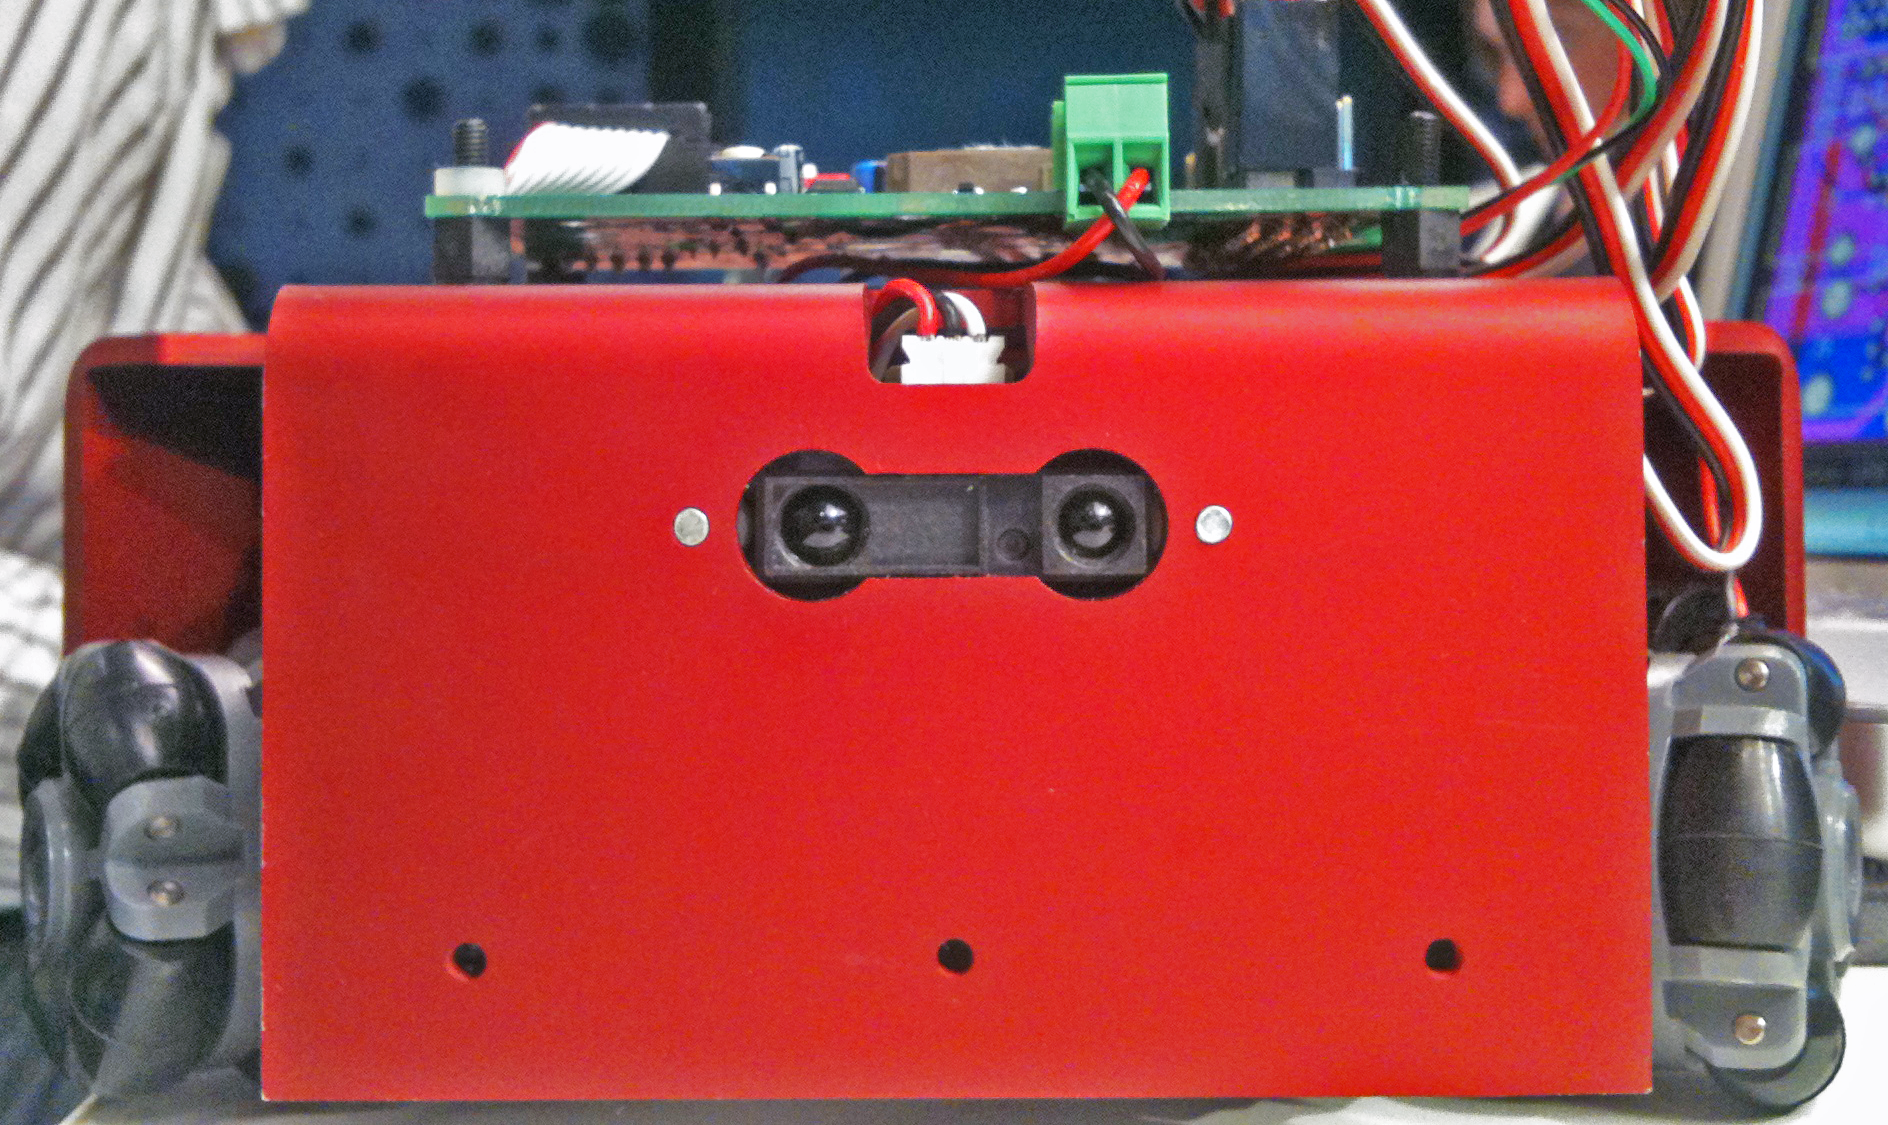
\includegraphics[width=0.4\textwidth]{img/cobot_face_sensor.png}}
    \subfloat[topview]{\label{fig:cobottop}
    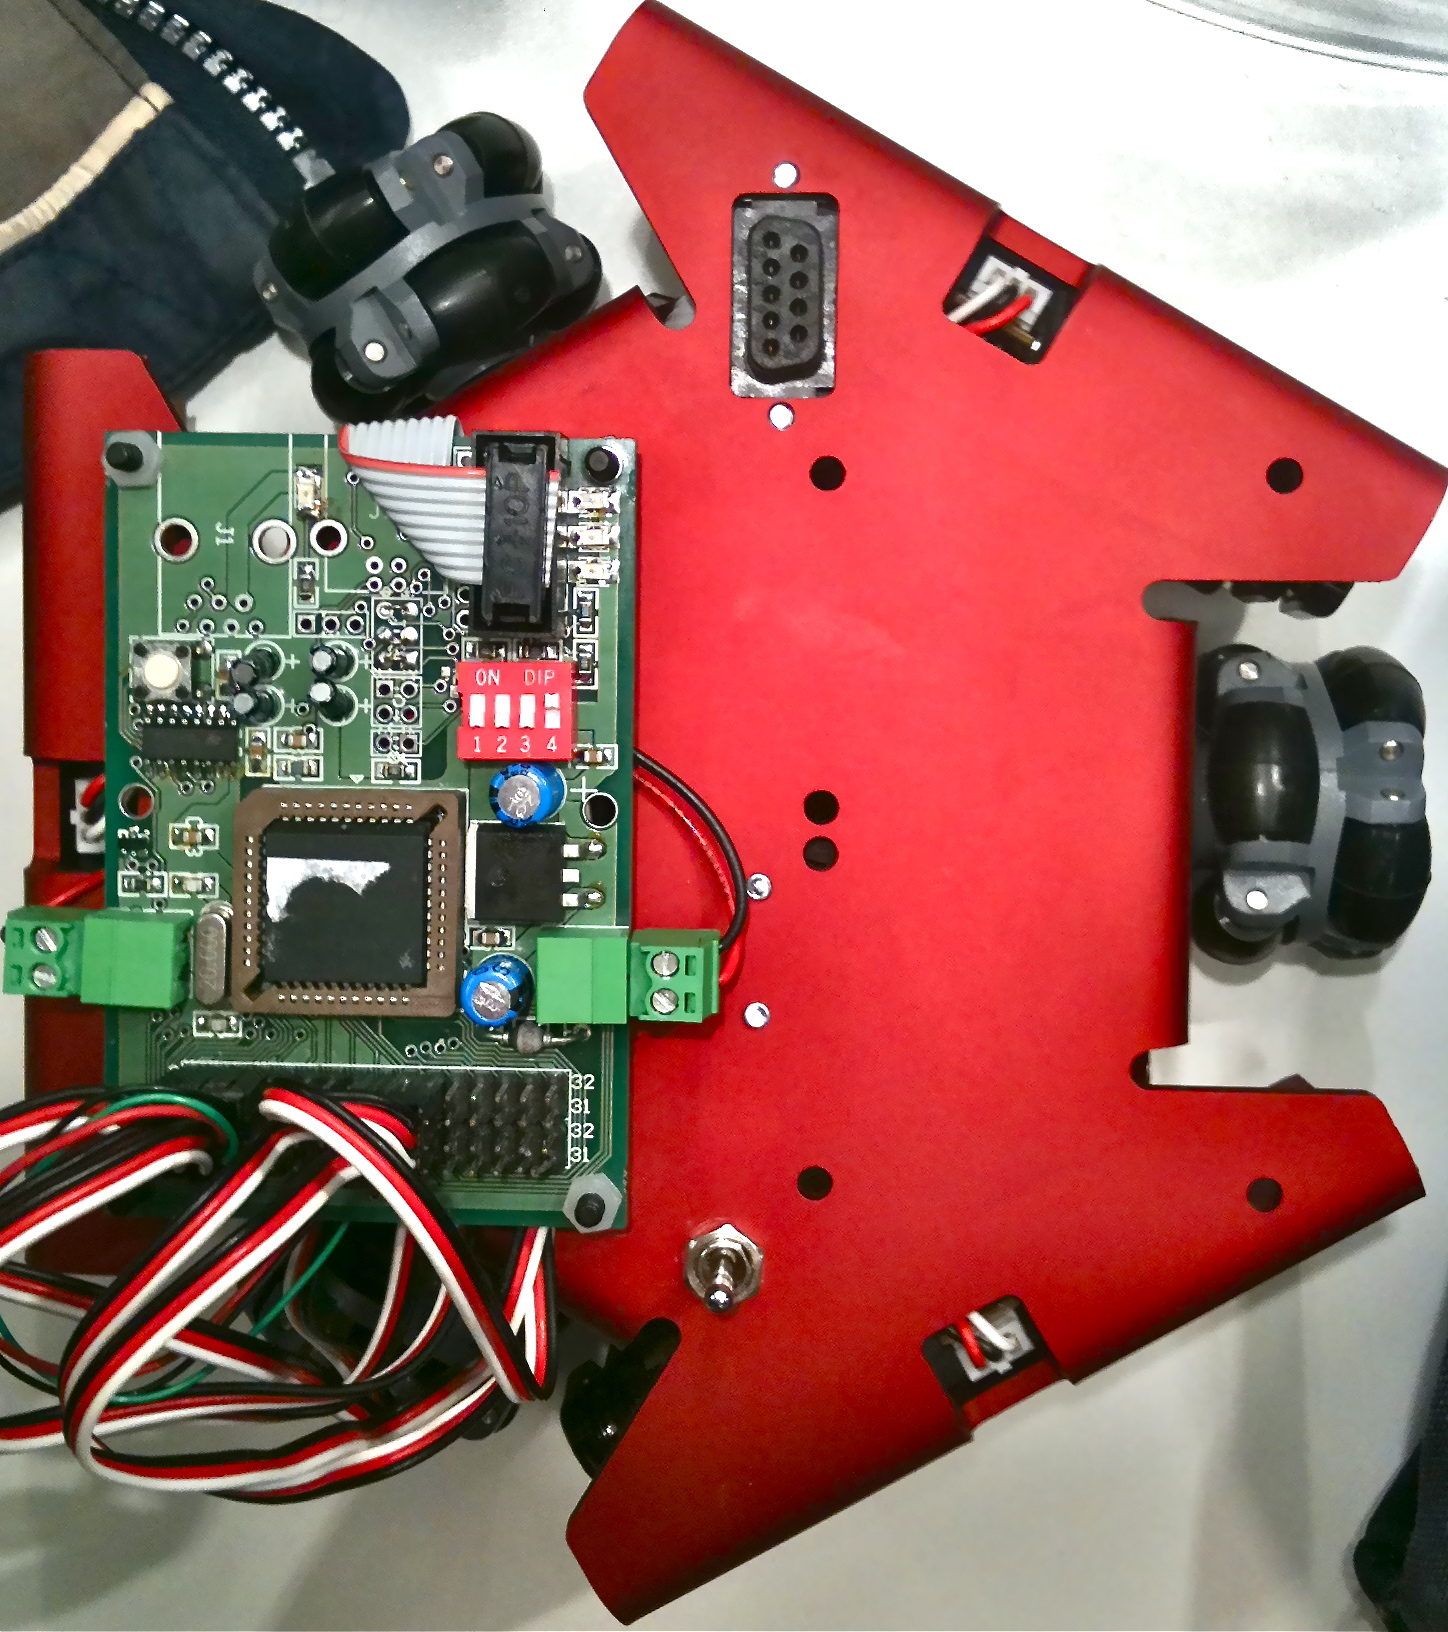
\includegraphics[width=0.4\textwidth]{img/cobot_top_view.png}}
    \caption{The Cobot}
    \label{fig:cobotviews}
\end{figure}

% }}}

The Cobot, the centrepiece of our project, is an adapted ``Jobot'',
re-christened to reflect the fact that our team reprogrammed the device in a
C-like language. The Jobot/Cobot is a battery powered, PIC microcontroller-based
mobile robot. It is about 10cm high and 25cm across. We disposed over three
Jobot/Cobot devices.

\subsubsection{Sun SPOTs}

\begin{figure}[H]
    \centering
    \subfloat[closed unit]{\label{fig:sunspot}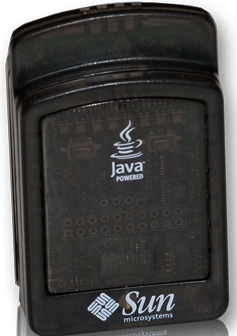
\includegraphics[width=0.4\textwidth]{img/sunspot.png}}
    \subfloat[Cobot cabling attached]{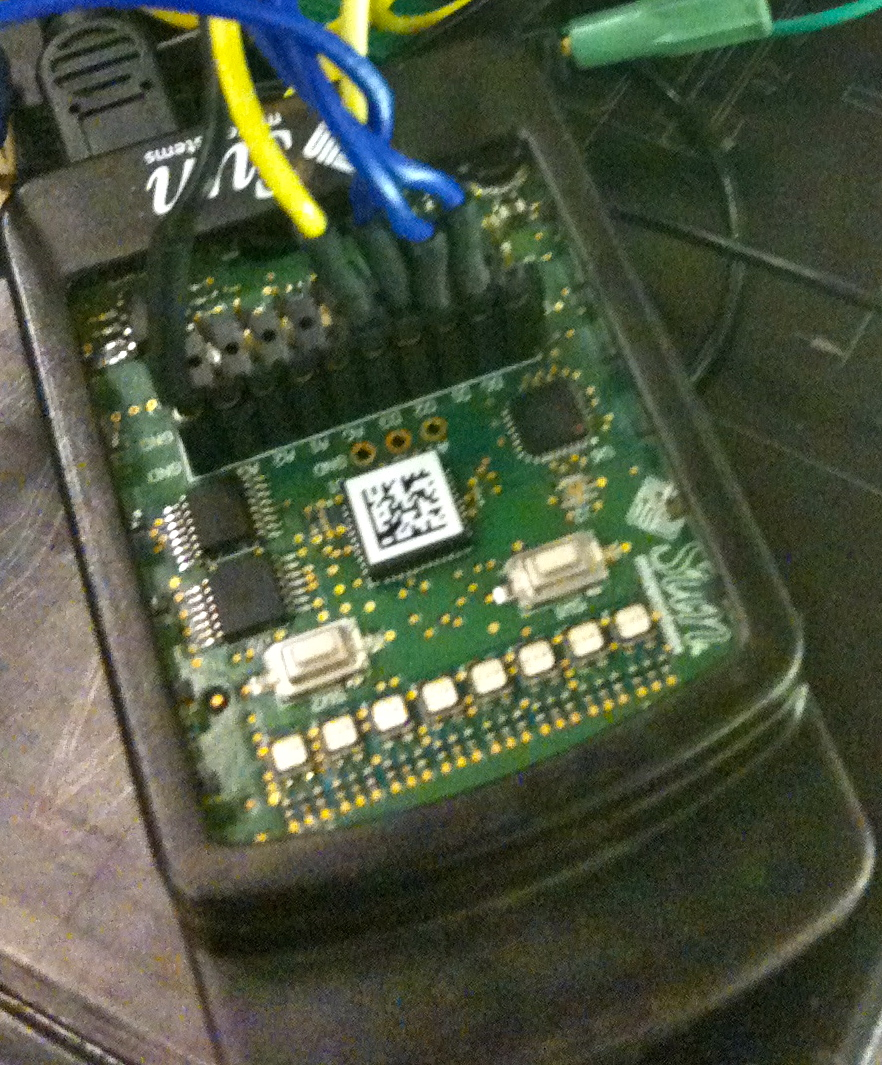
\includegraphics[width=0.4\textwidth]{img/sunspot_cabled.png}}
    \caption{The Sun SPOT}
    \label{fig:sunspotviews}
\end{figure}

Then, the Sun SPOT: the device intended to enhance the Cobot's sensing and
communications capabilities. Sun SPOTs are relatively new, battery powered
wireless sensor network devices from the Sun Labs stable. Our team received one
set, comprising three Sun SPOTs.

\subsubsection{Other hardware}

\noindent In addition to these two key components, our project relied heavily on
several hardware tools and devices, as follows: We used a portable digital
oscilloscope to measure voltages on the various I/O pins on the SUN SPOTs and
microcontroller boards (as well testing the odd misbehaving battery). A USB
compatible Microchip programming device served to load compiled code onto the
Cobot, via a specially attached 8P8C type connector on Cobot's microcontroller
board. We sourced a USB to RS-232 adapter cable to make the serial connection to
the Cobot. For the various I/O connections we made use of standard soldering
equipment. Department staff helped build pins and wires adapted for the Sun
SPOTs' as well as the Cobots' I/O connectors, and provided two potential
dividers for the bit banging bus.

\subsubsection{Software}

A number of off-the-shelf software tools complemented a software toolchain
developed especially by our team for this project. The former notably included
Microchip's compiler for the Cobot microcontroller, and Sun's development toolkit
for the Sun SPOT platform. Our own toolchain included scripts written in Python,
and an assemblage of open source UNIX-like command line utilities to link up the
software development, compilation and upload stages in the programming cycle.

% }}}

\subsection{Establishing COM-to-USB connection} % {{{
\label{sub:Establishing COM-to-USB connection}

In order to see if a Cobot or Hemisson is performing some action, it is wise to
write debug information to a file or serial port. In this case, the serial port
was available on both robots, providing a ``real-time'' view of the
robot's successive actions.

Sander developed some python code to be able to command the Hemisson robot using
a python console connected in combination with a serial port. The following code
is an implementation of most of the features available in the Hemisson GUI.
This code has two advantages: it is platform independent (enabling Mac and Linux
PCs to send commands the Hemisson) and enables the user to automate certain
actions, such as creating a software loop that causes the Hemisson to drive
around a rectangle.

\begin{Verbatim}[commandchars=\\\{\}]
\PY{c}{#!/usr/bin/env python}
\PY{c}{#}
\PY{c}{# This script is used to read and write data from/to the COM-to-USB port.}
\PY{c}{# Created by Sander van Veen <sandervv@gmail.com>, Jan 27, 2011.}
\PY{c}{# This script is public domain; feel free to do anything with it you want.}
\PY{c}{#}
\PY{c}{# Example invocation: $ python -i hemisson.py}

\PY{k+kn}{from} \PY{n+nn}{serial} \PY{k+kn}{import} \PY{n}{Serial}\PY{p}{,} \PY{n}{PARITY\PYZus{}NONE}\PY{p}{,} \PY{n}{EIGHTBITS}\PY{p}{,} \PY{n}{STOPBITS\PYZus{}ONE}
\PY{k+kn}{from} \PY{n+nn}{time} \PY{k+kn}{import} \PY{n}{sleep}

\PY{k}{class} \PY{n+nc}{HemissonException}\PY{p}{(}\PY{n+ne}{Exception}\PY{p}{)}\PY{p}{:}
    \PY{k}{def} \PY{n+nf}{\PYZus{}\PYZus{}init\PYZus{}\PYZus{}}\PY{p}{(}\PY{n+nb+bp}{self}\PY{p}{,} \PY{n}{value}\PY{p}{)}\PY{p}{:}
        \PY{n+nb+bp}{self}\PY{o}{.}\PY{n}{value} \PY{o}{=} \PY{n}{value}

    \PY{k}{def} \PY{n+nf}{\PYZus{}\PYZus{}str\PYZus{}\PYZus{}}\PY{p}{(}\PY{n+nb+bp}{self}\PY{p}{)}\PY{p}{:}
        \PY{k}{return} \PY{n+nb}{repr}\PY{p}{(}\PY{n+nb+bp}{self}\PY{o}{.}\PY{n}{value}\PY{p}{)}

\PY{k}{class} \PY{n+nc}{Hemisson}\PY{p}{:}
    \PY{k}{def} \PY{n+nf}{\PYZus{}\PYZus{}init\PYZus{}\PYZus{}}\PY{p}{(}\PY{n+nb+bp}{self}\PY{p}{)}\PY{p}{:}
        \PY{l+s+sd}{"""}
        \PY{l+s+sd}{Initialise the serial connection to the Hemisson robot.}
        \PY{l+s+sd}{"""}

        \PY{c}{# Initialise serial connection on /dev/ttyUSB0}
        \PY{n+nb+bp}{self}\PY{o}{.}\PY{n}{serial} \PY{o}{=} \PY{n}{Serial}\PY{p}{(}\PY{l+m+mi}{0}\PY{p}{)}
        \PY{n+nb+bp}{self}\PY{o}{.}\PY{n}{serial}\PY{o}{.}\PY{n}{setParity}\PY{p}{(}\PY{n}{PARITY\PYZus{}NONE}\PY{p}{)}
        \PY{n+nb+bp}{self}\PY{o}{.}\PY{n}{serial}\PY{o}{.}\PY{n}{setByteSize}\PY{p}{(}\PY{n}{EIGHTBITS}\PY{p}{)}
        \PY{n+nb+bp}{self}\PY{o}{.}\PY{n}{serial}\PY{o}{.}\PY{n}{setStopbits}\PY{p}{(}\PY{n}{STOPBITS\PYZus{}ONE}\PY{p}{)}
        \PY{n+nb+bp}{self}\PY{o}{.}\PY{n}{serial}\PY{o}{.}\PY{n}{setBaudrate}\PY{p}{(}\PY{l+m+mi}{115200}\PY{p}{)}

        \PY{c}{# Connection established, read welcome message from Hemisson.}
        \PY{k}{print} \PY{l+s}{'}\PY{l+s}{i Initialised serial connection }\PY{l+s}{"}\PY{l+s+si} \PY{n+nb+bp}{self}\PY{o}{.}\PY{n}{serial}\PY{o}{.}\PY{n}{portstr}
        \PY{n+nb+bp}{self}\PY{o}{.}\PY{n}{serial}\PY{o}{.}\PY{n}{write}\PY{p}{(}\PY{n+nb}{chr}\PY{p}{(}\PY{l+m+mi}{254}\PY{p}{)}\PY{o}{+}\PY{l+s}{'}\PY{l+s+se}{\PYZbs{}r}\PY{l+s}{'}\PY{p}{)}
        \PY{n+nb+bp}{self}\PY{o}{.}\PY{n}{readline}\PY{p}{(}\PY{p}{)}
        \PY{n+nb+bp}{self}\PY{o}{.}\PY{n}{readline}\PY{p}{(}\PY{p}{)}
        \PY{n+nb+bp}{self}\PY{o}{.}\PY{n}{readline}\PY{p}{(}\PY{p}{)}

    \PY{k}{def} \PY{n+nf}{\PYZus{}\PYZus{}delete\PYZus{}\PYZus{}}\PY{p}{(}\PY{n+nb+bp}{self}\PY{p}{)}\PY{p}{:}
        \PY{l+s+sd}{"""}
        \PY{l+s+sd}{Disconnect the serial connnection to the Hemisson robot.}
        \PY{l+s+sd}{"""}

        \PY{k}{print} \PY{l+s}{'}\PY{l+s}{i Destroying serial connection }\PY{l+s}{"}\PY{l+s+si} \PY{n+nb+bp}{self}\PY{o}{.}\PY{n}{serial}\PY{o}{.}\PY{n}{portstr}
        \PY{n+nb+bp}{self}\PY{o}{.}\PY{n}{write}\PY{p}{(}\PY{n+nb}{chr}\PY{p}{(}\PY{l+m+mi}{8}\PY{p}{)}\PY{p}{)}
        \PY{n+nb+bp}{self}\PY{o}{.}\PY{n}{serial}\PY{o}{.}\PY{n}{close}\PY{p}{(}\PY{p}{)}

    \PY{k}{def} \PY{n+nf}{beep}\PY{p}{(}\PY{n+nb+bp}{self}\PY{p}{,} \PY{n}{state}\PY{p}{)}\PY{p}{:}
        \PY{l+s+sd}{"""}
        \PY{l+s+sd}{Generates a continuous beep, depending on state (0 = Off, 1 = On).}
        \PY{l+s+sd}{"""}

        \PY{k}{if} \PY{n}{state} \PY{o+ow}{not} \PY{o+ow}{in} \PY{p}{(}\PY{l+m+mi}{0}\PY{p}{,} \PY{l+m+mi}{1}\PY{p}{)}\PY{p}{:}
            \PY{k}{raise} \PY{n}{HemissionException}\PY{p}{(}\PY{l+s}{'}\PY{l+s}{Beep state should be 0 (Off) or 1 (On).}\PY{l+s}{'}\PY{p}{)}

        \PY{n+nb+bp}{self}\PY{o}{.}\PY{n}{write}\PY{p}{(}\PY{l+s}{'}\PY{l+s}{H,}\PY{l+s+si} \PY{n}{state}\PY{p}{)}
        \PY{n+nb+bp}{self}\PY{o}{.}\PY{n}{readline}\PY{p}{(}\PY{p}{)}

    \PY{k}{def} \PY{n+nf}{drive}\PY{p}{(}\PY{n+nb+bp}{self}\PY{p}{)}\PY{p}{:}
        \PY{l+s+sd}{"""}
        \PY{l+s+sd}{Drive forward (setting both wheel's drive speed to '2').}
        \PY{l+s+sd}{"""}

        \PY{n+nb+bp}{self}\PY{o}{.}\PY{n}{set\PYZus{}speed}\PY{p}{(}\PY{l+m+mi}{2}\PY{p}{)}

    \PY{k}{def} \PY{n+nf}{get\PYZus{}switches}\PY{p}{(}\PY{n+nb+bp}{self}\PY{p}{)}\PY{p}{:}
        \PY{l+s+sd}{"""}
        \PY{l+s+sd}{Read the current status of the four top switches. Possible values are 0}
        \PY{l+s+sd}{(= robot's right handside) and 1 (= robot's left handside). The first}
        \PY{l+s+sd}{value is the value of the first switch from the front of the robot.}
        \PY{l+s+sd}{"""}

        \PY{n+nb+bp}{self}\PY{o}{.}\PY{n}{write}\PY{p}{(}\PY{l+s}{'}\PY{l+s}{I}\PY{l+s}{'}\PY{p}{)}
        \PY{n+nb+bp}{self}\PY{o}{.}\PY{n}{readline}\PY{p}{(}\PY{p}{)}

    \PY{k}{def} \PY{n+nf}{set\PYZus{}speed}\PY{p}{(}\PY{n+nb+bp}{self}\PY{p}{,} \PY{n}{left}\PY{p}{,} \PY{n}{right}\PY{o}{=}\PY{n+nb+bp}{None}\PY{p}{)}\PY{p}{:}
        \PY{l+s+sd}{"""}
        \PY{l+s+sd}{Set driving speed of left and right wheel. If only the left wheel drive}
        \PY{l+s+sd}{speed is given, the right wheel's drive speed is set to the left}
        \PY{l+s+sd}{wheel's drive speed.}
        \PY{l+s+sd}{"""}

        \PY{k}{if} \PY{n}{right} \PY{o}{==} \PY{n+nb+bp}{None}\PY{p}{:}
            \PY{n}{right} \PY{o}{=} \PY{n}{left}

        \PY{k}{if} \PY{o+ow}{not}\PY{p}{(} \PY{o}{-}\PY{l+m+mi}{9} \PY{o}{<}\PY{o}{=} \PY{n}{left} \PY{o}{<}\PY{o}{=} \PY{l+m+mi}{9} \PY{o+ow}{and} \PY{o}{-}\PY{l+m+mi}{9} \PY{o}{<}\PY{o}{=} \PY{n}{right} \PY{o}{<}\PY{o}{=} \PY{l+m+mi}{9}\PY{p}{)}\PY{p}{:}
            \PY{k}{raise} \PY{n}{HemissonException}\PY{p}{(}
                \PY{l+s}{'}\PY{l+s}{Keep the wheel drive speed value between -9 and 9.}\PY{l+s}{'}\PY{p}{)}

        \PY{n+nb+bp}{self}\PY{o}{.}\PY{n}{write}\PY{p}{(}\PY{l+s}{'}\PY{l+s}{D,}\PY{l+s+si}{%d}\PY{l+s}{,}\PY{l+s+si} \PY{p}{(}\PY{n}{left}\PY{p}{,} \PY{n}{right}\PY{p}{)}\PY{p}{)}
        \PY{n+nb+bp}{self}\PY{o}{.}\PY{n}{readline}\PY{p}{(}\PY{p}{)}

    \PY{k}{def} \PY{n+nf}{stop}\PY{p}{(}\PY{n+nb+bp}{self}\PY{p}{)}\PY{p}{:}
        \PY{l+s+sd}{"""}
        \PY{l+s+sd}{Stop moving forward (setting both wheel's drive speed to zero).}
        \PY{l+s+sd}{"""}

        \PY{n+nb+bp}{self}\PY{o}{.}\PY{n}{write}\PY{p}{(}\PY{l+s}{'}\PY{l+s}{D,0,0}\PY{l+s}{'}\PY{p}{)}
        \PY{n+nb+bp}{self}\PY{o}{.}\PY{n}{readline}\PY{p}{(}\PY{p}{)}

    \PY{k}{def} \PY{n+nf}{readline}\PY{p}{(}\PY{n+nb+bp}{self}\PY{p}{)}\PY{p}{:}
        \PY{l+s+sd}{"""}
        \PY{l+s+sd}{Read a single newline terminated line from the serial connection.}
        \PY{l+s+sd}{"""}

        \PY{k}{print} \PY{l+s}{'}\PY{l+s}{< }\PY{l+s+si} \PY{n+nb+bp}{self}\PY{o}{.}\PY{n}{serial}\PY{o}{.}\PY{n}{readline}\PY{p}{(}\PY{p}{)}\PY{p}{[}\PY{p}{:}\PY{o}{-}\PY{l+m+mi}{1}\PY{p}{]}

    \PY{k}{def} \PY{n+nf}{remote\PYZus{}version}\PY{p}{(}\PY{n+nb+bp}{self}\PY{p}{)}\PY{p}{:}
        \PY{l+s+sd}{"""}
        \PY{l+s+sd}{Display version of the HemiOS running on the connected Hemisson robot.}
        \PY{l+s+sd}{"""}

        \PY{n+nb+bp}{self}\PY{o}{.}\PY{n}{write}\PY{p}{(}\PY{l+s}{'}\PY{l+s}{B}\PY{l+s}{'}\PY{p}{)}
        \PY{n+nb+bp}{self}\PY{o}{.}\PY{n}{readline}\PY{p}{(}\PY{p}{)}

    \PY{k}{def} \PY{n+nf}{reset}\PY{p}{(}\PY{n+nb+bp}{self}\PY{p}{)}\PY{p}{:}
        \PY{l+s+sd}{"""}
        \PY{l+s+sd}{Reset the robot's processor as if the On/Off switch is cycled.}
        \PY{l+s+sd}{"""}

        \PY{n+nb+bp}{self}\PY{o}{.}\PY{n}{serial}\PY{o}{.}\PY{n}{write}\PY{p}{(}\PY{l+s}{'}\PY{l+s}{Z}\PY{l+s}{'}\PY{p}{)}
        \PY{n+nb+bp}{self}\PY{o}{.}\PY{n}{readline}\PY{p}{(}\PY{p}{)}

    \PY{k}{def} \PY{n+nf}{write}\PY{p}{(}\PY{n+nb+bp}{self}\PY{p}{,} \PY{n}{msg}\PY{p}{)}\PY{p}{:}
        \PY{l+s+sd}{"""}
        \PY{l+s+sd}{Write a message through the serial connection to the Hemisson robot.}
        \PY{l+s+sd}{"""}

        \PY{k}{print} \PY{l+s}{'}\PY{l+s}{> }\PY{l+s+si} \PY{n}{msg}
        \PY{n+nb+bp}{self}\PY{o}{.}\PY{n}{serial}\PY{o}{.}\PY{n}{write}\PY{p}{(}\PY{n}{msg}\PY{o}{+}\PY{l+s}{'}\PY{l+s+se}{\PYZbs{}n}\PY{l+s+se}{\PYZbs{}r}\PY{l+s}{'}\PY{p}{)}

\PY{k}{if} \PY{n}{\PYZus{}\PYZus{}name\PYZus{}\PYZus{}} \PY{o}{==} \PY{l+s}{'}\PY{l+s}{\PYZus{}\PYZus{}main\PYZus{}\PYZus{}}\PY{l+s}{'}\PY{p}{:}
    \PY{n}{robot} \PY{o}{=} \PY{n}{Hemisson}\PY{p}{(}\PY{p}{)}
    \PY{n}{robot}\PY{o}{.}\PY{n}{remote\PYZus{}version}\PY{p}{(}\PY{p}{)}
    \PY{n}{robot}\PY{o}{.}\PY{n}{get\PYZus{}switches}\PY{p}{(}\PY{p}{)}

    \PY{k}{for} \PY{n}{i} \PY{o+ow}{in} \PY{n+nb}{range}\PY{p}{(}\PY{l+m+mi}{4}\PY{p}{)}\PY{p}{:}
        \PY{n}{robot}\PY{o}{.}\PY{n}{set\PYZus{}speed}\PY{p}{(}\PY{l+m+mi}{4}\PY{p}{)}
        \PY{n}{sleep}\PY{p}{(}\PY{l+m+mi}{2}\PY{p}{)}
        \PY{n}{robot}\PY{o}{.}\PY{n}{set\PYZus{}speed}\PY{p}{(}\PY{o}{-}\PY{l+m+mi}{4}\PY{p}{,}\PY{l+m+mi}{4}\PY{p}{)}
        \PY{n}{sleep}\PY{p}{(}\PY{l+m+mf}{1.5}\PY{p}{)}

    \PY{n}{robot}\PY{o}{.}\PY{n}{stop}\PY{p}{(}\PY{p}{)}
\end{Verbatim}


\noindent We developed this utility to verify that communication over the
Hemisson's RS-232 COM port had been successful. When we started to develop code
for the Cobot, the utility was initially useless, since the Cobot did not have a
program in place to interpret the commands sent through the RS-232 COM port. The
Cobot had to be programmed from scratch. Once we had written the necessary
software handlers on the Cobot, though, our utility became useful once again.

% }}}

\subsection{Cobot} % {{{

% TODO: our initial approach

% TODO: write a general approach to solve the problems occurred during
% development of Cobot's code. -- what does this mean?

\subsubsection{Toolchain used to program the Cobot} % {{{
\label{ssub:Toolchain used to program the Cobot}

To program the Cobot we built a toolchain consisting of the following mixture of
pre-existing and custom-made software tools:

\begin{itemize}
    \item source code and compiled code for the Cobot, stored in a common
    working directory on UvA's science department servers;
    \item  the above directory mounted on a windows virtual machine and a Linux
    laptop over SSHFS\footnote{Secure SHell File System};
    \item Microchip's proprietary compiler for the Cobot's PIC microcontroller,
    running on the Windows virtual machine;
    \item our own python script, \texttt{compile.py}, running on the windows
    virtual machine: this automatically compiles the Cobot source code on the
    remote server when it changes;
    \item a python script on the Linux laptop to send commands to and read program
    output from the Cobot over the Cobot's RS-232 serial port;
\end{itemize}

\noindent First, we connected the shared directory using SSHFS:

\begin{verbatim}
$ sshfs USERNAME@deze.science.uva.nl:~/ ~/sremote -C -o cache=no
\end{verbatim}

The argument \texttt{-C} enables data compression during the transfer and
\texttt{-o cache=no} disables the file system cache (e.g. stat will respond with
the most recent data). With the file system cache left enabled, the overall
duration of the toolchain would have been larger due to the default four-second
file system cache. These four seconds were visible when the Mac machine running
the Windows VM waited for the source file to update, and again when the Linux
machine waited for the compiled hex file to update. Disabling the file system
cache reduced the overall toolchain process by four to eight seconds. Data
compression did not significantly reduce the overall process duration. We used
it because the transfers consisted largely of text files, which are especially
susceptible to compression.

Once we had the shared directory mounted on both the Linux and the Mac machine,
we were able to transfer data between those two.  \footnote{SSHFS is not easily
employed from within Windows: this was our motivation for running Windows as a
virtual machine on a Mac, which offers a more convenient implementation of
SSHFS.} The Windows virtual machine ran the compilation daemon (using \texttt{\$
python compile.py}) and the Linux machine ran the programming daemon (using
\texttt{python upload.py}).\footnote{See appendix for the source code of these
daemons.} Both daemons use the respective modification times of the source and
compiled hex files to trigger the necessary toolchain actions.

The programmer daemon used the ``piklab'' package (obtainable in Debian-based
distributions using: \texttt{sudo apt-get install piklab}) to write the hex file
to the Jobot. Note that piklab does not program the Jobot's microcontroller
directly, but through the ICD2 Programmer: it is not practicable to program the
Jobot directly. The daemon spawned a sub process to execute the Makefile's
default target. The default target executed the following commands in order to
program the Jobot:

\begin{verbatim}
$ sudo piklab-prog --port usb -p icd2 -d 18F450 -c connect
$ sudo piklab-prog --port usb -p icd2 -d 18F450 -c program file.hex
\end{verbatim}

These commands needed to be executed using \texttt{sudo} in order for piklab to
lock the USB-to-COM port. The second command also verified the programming
process, by checking whether the Jobot's microcontroller contained the uploaded
hex file.

\begin{figure}[H]
\hspace{-1.2in}
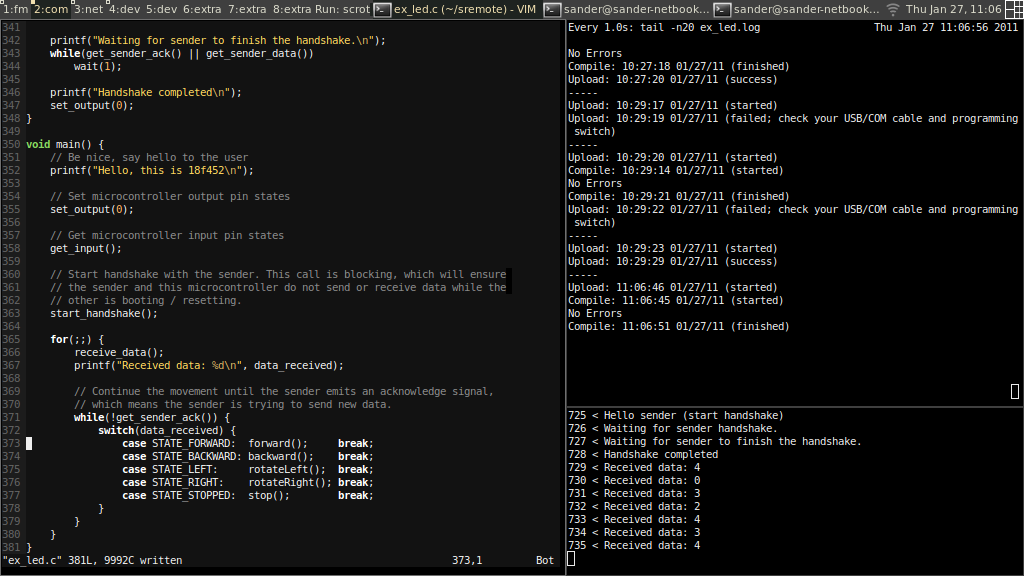
\includegraphics[scale=0.5]{img/workspace}
\caption{Workspace used to develop the Cobot's source code. On the left is Vim
(a highly configurable text editor built to enable efficient text editing). On
the top right is a build log displayed using the shell command: \texttt{\$
watch tail -n20 build.log}. On the bottom right is a reader for the
connection to the serial port: This simply displays all the messages sent to
the RS-232 COM port. These three windows are simply terminals. The Awesome
Window Manager is used to tile the windows together. Combined with the
toolchain, this constitutes a full-featured IDE dedicated to the Cobot.}
\end{figure}

For the Sun SPOT we used the recommended software, that is, the Sun SPOT
``manager'''s recommended installation. As the Sun SPOT development platform
might change with time, this set up is the most practical and reliable for Sun
SPOT related work. The SPOT manager handles all the environment variables needed
to get the program running.

% }}}

\subsubsection{Controlling the actuators} % {{{
\label{sub:Controlling the actuators}

Since there was no manual or documentation available about the toolchain, nor
about the internals of the Jobot, the first week's progress of this assignment
was slow. Most of the time, we were trying to solve problems and looking for
more information about the microcontroller and servos on the internet.
Eventually, when all tools for the toolchain were obtained and successfully
working together, we were able to run example code on the Jobot. This was the
breakthrough we were waiting for: we were able to write our own code and program
the Jobot with our compiled source code.

When we were using the PCH version of the CCS C compiler, we found some example
source code in the directory of the CCS C compiler. We modified the example code
to proof the microcontroller can do something, and programmed this modified code
on the Jobot's microcontroller:

\begin{Verbatim}[commandchars=\\\{\}]
\PY{c+c1}{// Device configuration: 20 Mhz processor and enable rs232,}
\PY{c+c1}{// which is the COM port. The COM port uses a baudrate of 9600.}
\PY{c+cp}{#}\PY{c+cp}{if defined(\PYZus{}\PYZus{}PCH\PYZus{}\PYZus{})}
\PY{c+cp}{#}\PY{c+cp}{include "18f452.h"}
\PY{c+cp}{#}\PY{c+cp}{fuses HS,NOPROTECT}
\PY{c+cp}{#}\PY{c+cp}{use delay(clock=20000000)}
\PY{c+cp}{#}\PY{c+cp}{use rs232(baud=9600, xmit=PIN\PYZus{}C6, rcv=PIN\PYZus{}C7)}
\PY{c+cp}{#}\PY{c+cp}{endif}

\PY{k+kt}{void} \PY{n+nf}{main}\PY{p}{(}\PY{p}{)} \PY{p}{\PYZob{}}
    \PY{c+c1}{// Set B pins to 'output' mode}
    \PY{n}{set\PYZus{}tris\PYZus{}b}\PY{p}{(}\PY{l+m+mi}{0}\PY{p}{)}\PY{p}{;}

    \PY{c+c1}{// Blink two LEDs (located on the microcontroller board).}
    \PY{c+c1}{// Wait for 2 ms between toggling the pins' value.}
    \PY{k}{while}\PY{p}{(}\PY{l+m+mi}{1}\PY{p}{)} \PY{p}{\PYZob{}}
        \PY{n}{output\PYZus{}high}\PY{p}{(}\PY{n}{PIN\PYZus{}B1}\PY{p}{)}\PY{p}{;}
        \PY{n}{delay\PYZus{}us}\PY{p}{(}\PY{l+m+mi}{2000}\PY{p}{)}\PY{p}{;}
        \PY{n}{output\PYZus{}low}\PY{p}{(}\PY{n}{PIN\PYZus{}B1}\PY{p}{)}\PY{p}{;}

        \PY{n}{output\PYZus{}high}\PY{p}{(}\PY{n}{PIN\PYZus{}B3}\PY{p}{)}\PY{p}{;}
        \PY{n}{delay\PYZus{}us}\PY{p}{(}\PY{l+m+mi}{2000}\PY{p}{)}\PY{p}{;}
        \PY{n}{output\PYZus{}low}\PY{p}{(}\PY{n}{PIN\PYZus{}B3}\PY{p}{)}\PY{p}{;}
    \PY{p}{\PYZcb{}}
\PY{p}{\PYZcb{}}
\end{Verbatim}


\noindent Note: The code shown above is a heavily modified version of the
example file \texttt{ex\_led.c}, which is part of the CCS C compiler's examples.

% }}}

% }}}

\subsection{Sun SPOTs} % {{{
\label{sec:sunspot}

The Sun SPOTs are used to control the Cobot. Initially, it was our intention to
stage communications between robots over the Sun SPOTs. We also intended for the
Sun SPOTs to receive and handle information from the robot sensors. For more
detailed information on the implementations see section \ref{sub:Sun SPOT
implementation}.

Both Sun SPOTs start up a \texttt{BootloaderListenerService}, so that we can
read the debug output in real-time on our computer, a useful feature. Both
Sun SPOTs extend the \texttt{javax.microedition.midlet.MIDlet} class, so that all
the functions the Sun SPOT needs to operate are available.

\subsubsection{Communication between the Sun SPOTs} % {{{
\label{subsec:comm}

The first order of business was getting the Sun SPOTs to communicate with each
other. A function enables the Sun SPOTs to start listening for information. It
is almost always necessary to filter some of the packets received in this way,
as other Sun SPOTs in the area could be sending packets not intended for the
current device.  Our team did not implement a robust system for ensuring that
only the intended packets were handled by our devices. We were able to progress
without such a mechanism since our Sun SPOTs were located away from other Sun
SPOTs during our project. However, an implementation can easily be added to our
code at a later stage. In the final version of our code, we do filter out
packets that do not contain valid commands. This avoids most unwanted traffic,
though the possibility that unwanted packets are handled in error remains open.

In order to understand the Sun SPOT sensors and communication functions, we
first wanted to develop a two-way transmission system that passes information
regarding one device's tilt to another device. We quickly learned that this
required the use of threads, since the devices often froze due to
desynchronisation without threads.

Once the threads were implemented, we began to successfully transmit the tilt
information between two Sun SPOTs. This would then serve as the basis for
communications between two robots, for remote control of a robot. The code
should lend itself to more difficult communications-related tasks.

% }}}

% }}}

\subsection{Bringing the pieces together} % {{{
\label{subsec:Bringing the pieces together}

For this project we used one Sun SPOT to determine the movement of the robot (by
measuring the tilt), and to send that information over a wireless connection to
the other Sun SPOT. Once it had received the datagram, the other device employed
bit banging to pass the desired movement information to the Cobot.

\subsubsection{Sun SPOT to Cobot: choosing a bus} % {{{
\label{ssub:bitbang}

Our initial plan was to transmit data between the Sun SPOT and the Cobot via the
$I^2C$ bus. Halfway through the project, though, technical issues transpired,
that made the $I^2C$ route impracticable. Namely, the Sun SPOT's I/O is
specified for 3V, whereas that of the Cobot is set at 5V. Connecting the
respective $I^2C$ ports directly risked damaging Sun SPOTs. Fortunately the
Cobot does register voltages of 2V and above, so that we had only to find a way
to step the Cobot's output voltage down to the Sun SPOTs' input voltage.

To overcome this data transmission problem, our department's staff suggested we
use ``bit-banging''. Bit-banging is a technique for serial communications using
software instead of dedicated hardware. This involves sending all the
information bit by bit from the software level, instead of sending the usual
packets of bytes in the form of a given data type. Bit banging requires good
control of how and when information is sent. Timing and synchronization between
parties becomes a key challenge. Bit-banging has its advantages: it is low-cost
and provides greater control. Perhaps most usefully, it can be used in just
about any programming language, on any system that can control communication
from the software level.

Our approach was to start by devising a deterministic bit banging protocol, that
is, a protocol that does not make use of a clock signal. This involved designing
a hand shaking protocol to align the devices to the same starting point on a
transfer. We then simulated our design between two Sun SPOTs.

\begin{figure}[H]
\label{fig:sunspotconnections}
\centering
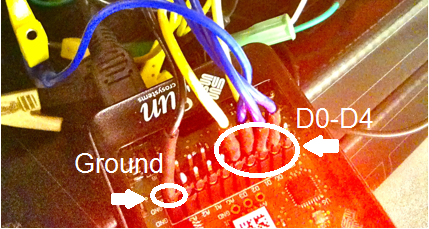
\includegraphics{img/sunspotconnections1.png}
\caption{The Sun SPOT with connections added to the ground and the digital
I/O}
\end{figure}

% }}}

\subsubsection{Bit banging: hardware bus} % {{{

At this stage we had both the Cobot ready to drive and had tested our
bit-banging algorithms between the Sun SPOTs. We could finally start putting the
pieces together, another challenge as it turned out.  The main obstacle lay in
the different voltages, described earlier in this section, which prevented a
direct connection between the Cobot's and the Sun SPOT's I/O ports. The solution
lay in assembling a potential divider, using the following equation:
\begin{equation} \label{eq:voltage} U = I*R \end{equation}

\begin{figure}[H]
    \label{fig:voltage_divider}
    \centering
    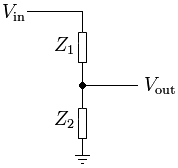
\includegraphics[scale=1]{img/voltage_divider.png}
    \caption{Potential divider}
\end{figure}

This comprised a wire with two serial resistances of 300k$\Omega$ and
200k$\Omega$ respectively. The result was that a 3V potential reached the Sun
Spot, with the remaining 2V leaking out to the ground. As is clear from figure
\ref{fig:handshaking}, this solution does not enable more complex information
transfers than those encoded in a high-low signal. More complex messages would
be distorted by the resistance between the sender and receiver.

\begin{figure}[H]
\label{fig:connection-schema}
\centering
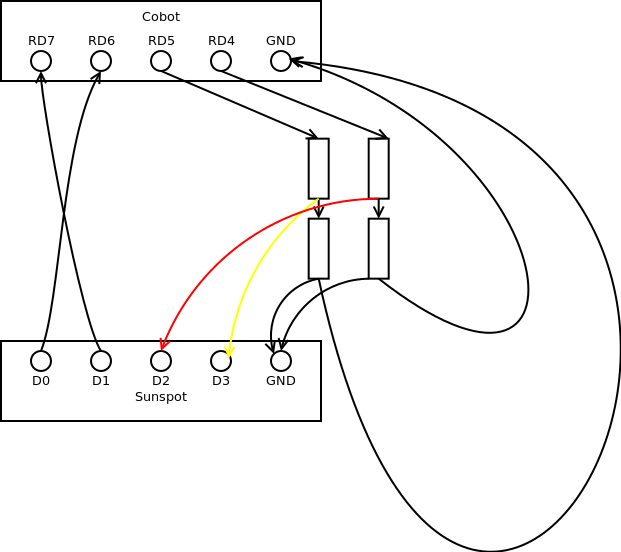
\includegraphics[scale=0.5]{img/connection-schema.png}
\caption{Schema of the the Sun SPOT and Cobot connected using a resistance.}
\end{figure}

Though our initial approach was to use timers provided in the Java framework to
transmit datagram between Sun SPOTs, we had to abandon these since we were
unable to guarantee that the timers on the respective devices would work
correctly. A deterministic approach involving a state machine was adopted
instead. The basic idea was straightforward: one could only transition from one
state to another, and acknowledge bits were continuously sent to both sides. See
figure \ref{fig:handshaking} for an illustration of the deterministic bit
banging protocol.

\begin{figure}[H]
\label{fig:handshaking}
\centering
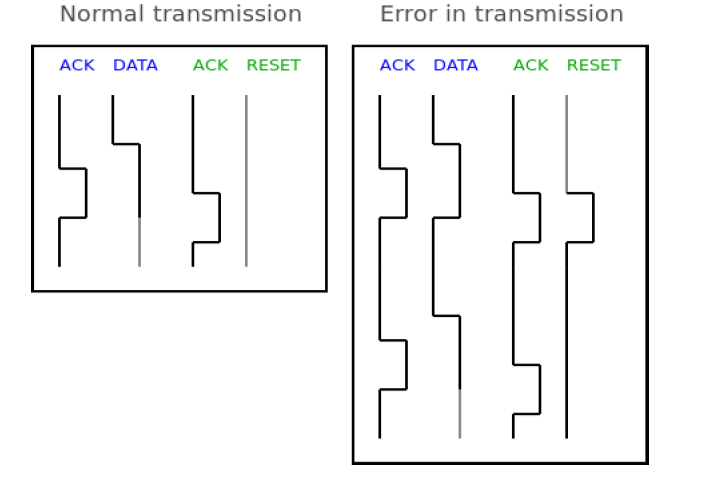
\includegraphics[width=11cm]{img/handshaking.png}
\caption{The left image is a bit diagram of a normal transmission and the right
image is a simplified example of an error occurring during transmission. To send
one bit from a device (blue labelled lines: sender) to another device (green
labelled lines: receiver), first requires putting the data pin on the value one
wants to send. Then one raises the ACK flag. Now, the receiver knows the sender
is ready to send a bit.  When the receiver sees the sender's ACK flag, the
receiver reads the value of the data pin and raises their acknowledge flag. When
the receiver raises their ACK flag, the sender knows the message bit has been
received. The sender lowers their acknowledge flag, and the receiver responds by
lowering their own ACK flag as too. When both ACK flags are down, the process
starts over. There is also a reset flag, which indicates a that restart of the
whole process is required.  The receiver sets their reset flag when an invalid
value is received.}
\end{figure}

\begin{figure}[H]
\label{fig:cobot-sun-spot}
\centering
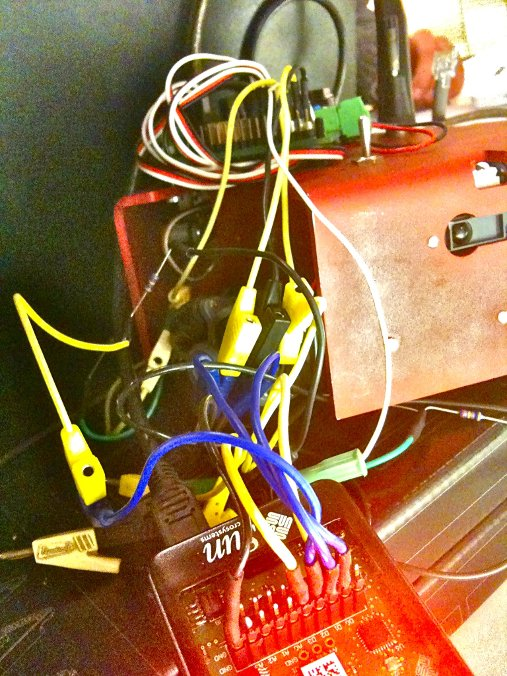
\includegraphics[scale=0.5]{img/cobot_and_sunspot.jpg}
\caption{Custom-made bit banging connection between Sun SPOT \& Cobot.}
\end{figure}

% }}}

% }}}

% }}}

\pagebreak

\section{Implementation} % {{{
\label{sec:Implementation}

\subsection{Cobot implementation} % {{{
\label{sub:Cobot implementation}

Since there was no manual or documentation available regarding the toolchain
(there was no information available about what tools should be used), nor about
the internals of the Jobot, the first week's progress for this assignment was
slow. We spent much of our time overcoming seemingly preliminary obstacles, and
searched the internet for documentation or specifications regarding the
microcontroller and servos.  Eventually, when all tools for the toolchain were
obtained and successfully integrated, we were able to run example code on the
Cobot. This was the breakthrough we had been waiting for: we were able to write
our own code and load the Cobot with the programs we compiled.

\subsubsection{The first working program} % {{{
\label{ssub:The first working example source code}

Whilst using the PCH version of the CCS C compiler, we found some example
source code in the Compiler's directory. We modified the example code
and used this to establish that microcontroller worked as intended. We loaded the following code onto the Cobot's microcontroller:

\begin{Verbatim}[commandchars=\\\{\}]
\PY{c+c1}{// Device configuration: 20 Mhz processor and enable rs232,}
\PY{c+c1}{// which is the COM port. The COM port uses a baudrate of 9600.}
\PY{c+cp}{#}\PY{c+cp}{if defined(\PYZus{}\PYZus{}PCH\PYZus{}\PYZus{})}
\PY{c+cp}{#}\PY{c+cp}{include "18f452.h"}
\PY{c+cp}{#}\PY{c+cp}{fuses HS,NOPROTECT}
\PY{c+cp}{#}\PY{c+cp}{use delay(clock=20000000)}
\PY{c+cp}{#}\PY{c+cp}{use rs232(baud=9600, xmit=PIN\PYZus{}C6, rcv=PIN\PYZus{}C7)}
\PY{c+cp}{#}\PY{c+cp}{endif}

\PY{k+kt}{void} \PY{n+nf}{main}\PY{p}{(}\PY{p}{)} \PY{p}{\PYZob{}}
    \PY{c+c1}{// Set B pins to 'output' mode}
    \PY{n}{set\PYZus{}tris\PYZus{}b}\PY{p}{(}\PY{l+m+mi}{0}\PY{p}{)}\PY{p}{;}

    \PY{c+c1}{// Blink two LEDs (located on the microcontroller board).}
    \PY{c+c1}{// Wait for 2 ms between toggling the pins' value.}
    \PY{k}{while}\PY{p}{(}\PY{l+m+mi}{1}\PY{p}{)} \PY{p}{\PYZob{}}
        \PY{n}{output\PYZus{}high}\PY{p}{(}\PY{n}{PIN\PYZus{}B1}\PY{p}{)}\PY{p}{;}
        \PY{n}{delay\PYZus{}us}\PY{p}{(}\PY{l+m+mi}{2000}\PY{p}{)}\PY{p}{;}
        \PY{n}{output\PYZus{}low}\PY{p}{(}\PY{n}{PIN\PYZus{}B1}\PY{p}{)}\PY{p}{;}

        \PY{n}{output\PYZus{}high}\PY{p}{(}\PY{n}{PIN\PYZus{}B3}\PY{p}{)}\PY{p}{;}
        \PY{n}{delay\PYZus{}us}\PY{p}{(}\PY{l+m+mi}{2000}\PY{p}{)}\PY{p}{;}
        \PY{n}{output\PYZus{}low}\PY{p}{(}\PY{n}{PIN\PYZus{}B3}\PY{p}{)}\PY{p}{;}
    \PY{p}{\PYZcb{}}
\PY{p}{\PYZcb{}}
\end{Verbatim}


\noindent Note: The code shown above is a heavily modified version of the
example file \texttt{ex\_led.c}, which is part of the CCS C compiler's examples.

% }}}

\subsubsection{Cobot's data receiver and error checker} % {{{
\label{ssub:Cobot's data receiver and error checker}

Transferring data between the Cobot and Sun SPOT is a bit fragile due to
external dependencies. For example, if a single bit is somehow not set to HIGH
when it should be, all the following and preceding bits of the message are
useless. To prevent these external dependencies from corrupting the messages, we
implemented a simple form of error checking: send the message twice and compare
the first message with the second. It was also possible to implement a more
robust error checking algorithm (e.g. Hamming code), but that would have been
overkill, since we were just sending messages of three bits. Our simple error
checker would do.

\begin{Verbatim}[commandchars=\\\{\}]
\PY{c+c1}{// Buffer for data receiving}
\PY{k+kt}{int} \PY{n}{data\PYZus{}previous}\PY{p}{,} \PY{n}{data\PYZus{}current}\PY{p}{,} \PY{n}{data\PYZus{}received}\PY{p}{,} \PY{n}{receive\PYZus{}round}\PY{p}{;}
\PY{k+kt}{int} \PY{n}{b}\PY{p}{,} \PY{n}{bit\PYZus{}count} \PY{o}{=} \PY{l+m+mi}{3}\PY{p}{;}

\PY{k+kt}{void} \PY{n+nf}{receive\PYZus{}data}\PY{p}{(}\PY{p}{)} \PY{p}{\PYZob{}}
    \PY{c+c1}{// Clear data buffers}
    \PY{n}{data\PYZus{}received} \PY{o}{=} \PY{n}{data\PYZus{}previous} \PY{o}{=} \PY{n}{data\PYZus{}current} \PY{o}{=} \PY{l+m+mi}{0}\PY{p}{;}

    \PY{c+c1}{// Receive two times (= "rounds") three bits. Most significant bits are}
    \PY{c+c1}{// transmitted first (thus from left to right)}
    \PY{k}{for}\PY{p}{(} \PY{n}{receive\PYZus{}round} \PY{o}{=} \PY{l+m+mi}{0}\PY{p}{;} \PY{n}{receive\PYZus{}round} \PY{o}{<} \PY{l+m+mi}{2}\PY{p}{;} \PY{n}{receive\PYZus{}round}\PY{o}{+}\PY{o}{+} \PY{p}{)} \PY{p}{\PYZob{}}
        \PY{k}{for}\PY{p}{(}\PY{n}{b} \PY{o}{=} \PY{l+m+mi}{0}\PY{p}{;} \PY{n}{b} \PY{o}{<} \PY{n}{bit\PYZus{}count}\PY{p}{;} \PY{n}{b}\PY{o}{+}\PY{o}{+}\PY{p}{)} \PY{p}{\PYZob{}}
            \PY{c+c1}{//printf("round: %d, b: %d\PYZbs{}n", receive\PYZus{}round, bit\PYZus{}count - b);}
            \PY{n}{debug}\PY{p}{(}\PY{l+s}{"}\PY{l+s}{get\PYZus{}sender\PYZus{}ack() first}\PY{l+s+se}{\PYZbs{}n}\PY{l+s}{"}\PY{p}{)}\PY{p}{;}
            \PY{k}{while}\PY{p}{(}\PY{o}{!}\PY{n}{get\PYZus{}sender\PYZus{}ack}\PY{p}{(}\PY{p}{)}\PY{p}{)}
                \PY{n}{wait}\PY{p}{(}\PY{l+m+mi}{1}\PY{p}{)}\PY{p}{;}

            \PY{n}{debug}\PY{p}{(}\PY{l+s}{"}\PY{l+s}{get\PYZus{}sender\PYZus{}data()}\PY{l+s+se}{\PYZbs{}n}\PY{l+s}{"}\PY{p}{)}\PY{p}{;}
            \PY{n}{data\PYZus{}current} \PY{o}{|}\PY{o}{=} \PY{n}{get\PYZus{}sender\PYZus{}data}\PY{p}{(}\PY{p}{)} \PY{o}{<}\PY{o}{<} \PY{p}{(}\PY{n}{bit\PYZus{}count}\PY{o}{-}\PY{n}{b}\PY{o}{-}\PY{l+m+mi}{1}\PY{p}{)}\PY{p}{;}

            \PY{c+c1}{// First round is simply storing the data and emits an acknowledge}
            \PY{c+c1}{// signal (= 1). The second round is used for error checking. The}
            \PY{c+c1}{// second round will emit an acknowledge signal when the data is}
            \PY{c+c1}{// properly transmitted / received. The second round will send an}
            \PY{c+c1}{// acknowledge and reset signal (= 3), when the current data bit is}
            \PY{c+c1}{// not matching data of the previous round.}
            \PY{k}{if}\PY{p}{(}\PY{n}{receive\PYZus{}round} \PY{o}{=}\PY{o}{=} \PY{l+m+mi}{0}
                    \PY{o}{|}\PY{o}{|} \PY{p}{(}\PY{n}{data\PYZus{}previous} \PY{o}{&} \PY{p}{(}\PY{l+m+mi}{1}\PY{o}{<}\PY{o}{<}\PY{p}{(}\PY{n}{bit\PYZus{}count}\PY{o}{-}\PY{n}{b}\PY{o}{-}\PY{l+m+mi}{1}\PY{p}{)}\PY{p}{)}\PY{p}{)}
                            \PY{o}{=}\PY{o}{=} \PY{p}{(}\PY{n}{data\PYZus{}current} \PY{o}{&} \PY{p}{(}\PY{l+m+mi}{1}\PY{o}{<}\PY{o}{<}\PY{p}{(}\PY{n}{bit\PYZus{}count}\PY{o}{-}\PY{n}{b}\PY{o}{-}\PY{l+m+mi}{1}\PY{p}{)}\PY{p}{)}\PY{p}{)}\PY{p}{)}
                \PY{n}{set\PYZus{}output}\PY{p}{(}\PY{l+m+mi}{1}\PY{p}{)}\PY{p}{;}
            \PY{k}{else} \PY{p}{\PYZob{}}
                \PY{n}{debug}\PY{p}{(}\PY{l+s}{"}\PY{l+s}{Error during transmission}\PY{l+s+se}{\PYZbs{}n}\PY{l+s}{"}\PY{p}{)}\PY{p}{;}
                \PY{n}{set\PYZus{}output}\PY{p}{(}\PY{l+m+mi}{3}\PY{p}{)}\PY{p}{;}

                \PY{c+c1}{// Wait until the sender sees the acknowledge and reset signal.}
                \PY{c+c1}{// When the sender emits his acknowledge signal, the receive}
                \PY{c+c1}{// procedure is restarted.}
                \PY{k}{while}\PY{p}{(}\PY{n}{get\PYZus{}sender\PYZus{}ack}\PY{p}{(}\PY{p}{)}\PY{p}{)}
                    \PY{n}{wait}\PY{p}{(}\PY{l+m+mi}{1}\PY{p}{)}\PY{p}{;}
                \PY{n}{set\PYZus{}output}\PY{p}{(}\PY{l+m+mi}{0}\PY{p}{)}\PY{p}{;}
                \PY{k}{return} \PY{n}{receive\PYZus{}data}\PY{p}{(}\PY{p}{)}\PY{p}{;}
            \PY{p}{\PYZcb{}}

            \PY{n}{debug}\PY{p}{(}\PY{l+s}{"}\PY{l+s}{get\PYZus{}sender\PYZus{}ack() last}\PY{l+s+se}{\PYZbs{}n}\PY{l+s}{"}\PY{p}{)}\PY{p}{;}
            \PY{k}{while}\PY{p}{(}\PY{n}{get\PYZus{}sender\PYZus{}ack}\PY{p}{(}\PY{p}{)}\PY{p}{)}
                \PY{n}{wait}\PY{p}{(}\PY{l+m+mi}{1}\PY{p}{)}\PY{p}{;}

            \PY{n}{set\PYZus{}output}\PY{p}{(}\PY{l+m+mi}{0}\PY{p}{)}\PY{p}{;}
        \PY{p}{\PYZcb{}}

        \PY{n}{data\PYZus{}previous} \PY{o}{=} \PY{n}{data\PYZus{}current}\PY{p}{;}
        \PY{n}{data\PYZus{}current} \PY{o}{=} \PY{l+m+mi}{0}\PY{p}{;}
    \PY{p}{\PYZcb{}}

    \PY{n}{data\PYZus{}received} \PY{o}{=} \PY{n}{data\PYZus{}previous}\PY{p}{;}
\PY{p}{\PYZcb{}}
\end{Verbatim}


\noindent The expression \texttt{bit\_count-b-1} may look a little silly, but is
needed, since the CCS C compiler does not handle all branch conditions well. For
example, it does not handle these loops as expected:

\begin{Verbatim}[commandchars=\\\{\}]
\PY{k+kt}{void} \PY{n+nf}{main}\PY{p}{(}\PY{p}{)} \PY{p}{\PYZob{}}
    \PY{k+kt}{int} \PY{n}{i}\PY{p}{;}

    \PY{c+c1}{// Normal loop}
    \PY{k}{for}\PY{p}{(}\PY{n}{i} \PY{o}{=} \PY{l+m+mi}{0}\PY{p}{;} \PY{n}{i} \PY{o}{<} \PY{l+m+mi}{3}\PY{p}{;} \PY{n}{i}\PY{o}{+}\PY{o}{+}\PY{p}{)} \PY{p}{\PYZob{}}
        \PY{n}{printf}\PY{p}{(}\PY{l+s}{"}\PY{l+s}{i = %d}\PY{l+s+se}{\PYZbs{}n}\PY{l+s}{"}\PY{p}{,} \PY{n}{i}\PY{p}{)}\PY{p}{;}
    \PY{p}{\PYZcb{}}

    \PY{c+c1}{// Reverse loop}
    \PY{k}{for}\PY{p}{(}\PY{n}{i} \PY{o}{=} \PY{l+m+mi}{2}\PY{p}{;} \PY{n}{i} \PY{o}{>}\PY{o}{=} \PY{l+m+mi}{0}\PY{p}{;} \PY{n}{i}\PY{o}{-}\PY{o}{-}\PY{p}{)} \PY{p}{\PYZob{}}
        \PY{n}{printf}\PY{p}{(}\PY{l+s}{"}\PY{l+s}{i = %d}\PY{l+s+se}{\PYZbs{}n}\PY{l+s}{"}\PY{p}{,} \PY{n}{i}\PY{p}{)}\PY{p}{;}
    \PY{p}{\PYZcb{}}
\PY{p}{\PYZcb{}}
\end{Verbatim}


\noindent The first loop does print \text{i} with 0, 1 and 2. The second loop
prints a reversed output of the first loop, except that it does not stop after
0. The loop continues and prints output towards minus infinity.  We tackled this
by rewriting the loop of the receiver to the expression stated above.  As you
can imagine, the absence of such simple operations poses quite a challenge to
anyone wishing to implement a driver for a robot.

% }}}

\subsubsection{Cobot's handshake and start} % {{{
\label{ssub:Cobot's handshake and start}

In order to start the communication between the Cobot and Sun SPOT in a proper
way, we implemented a handshake protocol to ensure the Cobot and Sun SPOT are in
the same state. Before we implemented the handshake, the Sun SPOT or Cobot sent
some data to its output pins which caused the other device to do some unwanted
action. To prevent this from happening, the handshake protocol ensures both
devices are ready for action.

The handshake is simple: put both pins up on both devices and wait until both
pins on both devices are down. This handshake protocol is defined as a state
machine. The Sun SPOT requires the Cobot's output pins to be high. Once those
pins are high, the Sun SPOT raises both pins. The Cobot detects both pins of the
Sun SPOT are high and will wait until the Sun SPOT's pins are both low again.
The Sun SPOT waits a few milliseconds before lowering its pins. When the Sun
SPOT has lowered its pins, the Cobot will lower its pins and the handshake is
completed. Below is the initialisation code of the Cobot:

\begin{Verbatim}[commandchars=\\\{\}]
\PY{k+kt}{void} \PY{n+nf}{start\PYZus{}handshake}\PY{p}{(}\PY{p}{)} \PY{p}{\PYZob{}}
    \PY{n}{printf}\PY{p}{(}\PY{l+s}{"}\PY{l+s}{Hello sender (start handshake)}\PY{l+s+se}{\PYZbs{}n}\PY{l+s}{"}\PY{p}{)}\PY{p}{;}
    \PY{n}{set\PYZus{}output}\PY{p}{(}\PY{l+m+mi}{3}\PY{p}{)}\PY{p}{;}

    \PY{n}{printf}\PY{p}{(}\PY{l+s}{"}\PY{l+s}{Waiting for sender handshake.}\PY{l+s+se}{\PYZbs{}n}\PY{l+s}{"}\PY{p}{)}\PY{p}{;}
    \PY{k}{while}\PY{p}{(}\PY{o}{!}\PY{n}{get\PYZus{}sender\PYZus{}ack}\PY{p}{(}\PY{p}{)} \PY{o}{|}\PY{o}{|} \PY{o}{!}\PY{n}{get\PYZus{}sender\PYZus{}data}\PY{p}{(}\PY{p}{)}\PY{p}{)}
        \PY{n}{wait}\PY{p}{(}\PY{l+m+mi}{1}\PY{p}{)}\PY{p}{;}

    \PY{n}{printf}\PY{p}{(}\PY{l+s}{"}\PY{l+s}{Waiting for sender to finish the handshake.}\PY{l+s+se}{\PYZbs{}n}\PY{l+s}{"}\PY{p}{)}\PY{p}{;}
    \PY{k}{while}\PY{p}{(}\PY{n}{get\PYZus{}sender\PYZus{}ack}\PY{p}{(}\PY{p}{)} \PY{o}{|}\PY{o}{|} \PY{n}{get\PYZus{}sender\PYZus{}data}\PY{p}{(}\PY{p}{)}\PY{p}{)}
        \PY{n}{wait}\PY{p}{(}\PY{l+m+mi}{1}\PY{p}{)}\PY{p}{;}

    \PY{n}{printf}\PY{p}{(}\PY{l+s}{"}\PY{l+s}{Handshake completed}\PY{l+s+se}{\PYZbs{}n}\PY{l+s}{"}\PY{p}{)}\PY{p}{;}
    \PY{n}{set\PYZus{}output}\PY{p}{(}\PY{l+m+mi}{0}\PY{p}{)}\PY{p}{;}
\PY{p}{\PYZcb{}}

\PY{k+kt}{void} \PY{n+nf}{main}\PY{p}{(}\PY{p}{)} \PY{p}{\PYZob{}}
    \PY{c+c1}{// Be nice, say hello to the user}
    \PY{n}{printf}\PY{p}{(}\PY{l+s}{"}\PY{l+s}{Hello, this is 18f452}\PY{l+s+se}{\PYZbs{}n}\PY{l+s}{"}\PY{p}{)}\PY{p}{;}

    \PY{c+c1}{// Set microcontroller output pin states}
    \PY{c+c1}{// Get microcontroller input pin states}
    \PY{n}{set\PYZus{}output}\PY{p}{(}\PY{l+m+mi}{0}\PY{p}{)}\PY{p}{;}
    \PY{n}{get\PYZus{}input}\PY{p}{(}\PY{p}{)}\PY{p}{;}

    \PY{c+c1}{// Start handshake with the sender. This call is blocking, which will ensure}
    \PY{c+c1}{// the sender and this microcontroller do not send or receive data while the}
    \PY{c+c1}{// other is booting / resetting.}
    \PY{n}{start\PYZus{}handshake}\PY{p}{(}\PY{p}{)}\PY{p}{;}

    \PY{k}{for}\PY{p}{(}\PY{p}{;}\PY{p}{;}\PY{p}{)} \PY{p}{\PYZob{}}
        \PY{n}{receive\PYZus{}data}\PY{p}{(}\PY{p}{)}\PY{p}{;}
        \PY{n}{printf}\PY{p}{(}\PY{l+s}{"}\PY{l+s}{Received data: %d}\PY{l+s+se}{\PYZbs{}n}\PY{l+s}{"}\PY{p}{,} \PY{n}{data\PYZus{}received}\PY{p}{)}\PY{p}{;}

        \PY{c+c1}{// Continue the movement until the sender emits an acknowledge signal,}
        \PY{c+c1}{// which means the sender is trying to send new data.}
        \PY{k}{while}\PY{p}{(}\PY{o}{!}\PY{n}{get\PYZus{}sender\PYZus{}ack}\PY{p}{(}\PY{p}{)}\PY{p}{)} \PY{p}{\PYZob{}}
            \PY{k}{switch}\PY{p}{(}\PY{n}{data\PYZus{}received}\PY{p}{)} \PY{p}{\PYZob{}}
                \PY{k}{case} \PY{n}{STATE\PYZus{}FORWARD}:  \PY{n}{forward}\PY{p}{(}\PY{p}{)}\PY{p}{;}     \PY{k}{break}\PY{p}{;}
                \PY{k}{case} \PY{n}{STATE\PYZus{}BACKWARD}: \PY{n}{backward}\PY{p}{(}\PY{p}{)}\PY{p}{;}    \PY{k}{break}\PY{p}{;}
                \PY{k}{case} \PY{n}{STATE\PYZus{}LEFT}:     \PY{n}{rotateLeft}\PY{p}{(}\PY{p}{)}\PY{p}{;}  \PY{k}{break}\PY{p}{;}
                \PY{k}{case} \PY{n}{STATE\PYZus{}RIGHT}:    \PY{n}{rotateRight}\PY{p}{(}\PY{p}{)}\PY{p}{;} \PY{k}{break}\PY{p}{;}
                \PY{k}{case} \PY{n}{STATE\PYZus{}STOPPED}:  \PY{n}{stop}\PY{p}{(}\PY{p}{)}\PY{p}{;}        \PY{k}{break}\PY{p}{;}
            \PY{p}{\PYZcb{}}
        \PY{p}{\PYZcb{}}
    \PY{p}{\PYZcb{}}
\PY{p}{\PYZcb{}}
\end{Verbatim}


% }}}

% }}}

\subsection{Sun SPOT implementation} % {{{
\label{sub:Sun SPOT implementation}

For this project we used one Sun SPOT to determine the movement of the robot (by
measuring the tilt) and sending that information using a wireless connection to
the other Sun SPOT. The other Sun SPOT receives the datagram and uses
bit banging to pass the relevant movement information to the Cobot. 

Both Sun SPOTs start up a \texttt{BootloaderListenerService}, so that we can
read the debug output in real-time on our computer, a useful feature. Both
Sun SPOTs extend the \texttt{javax.microedition.midlet.MIDlet} class, so that all
the functions the Sun SPOT needs to operate are available.

\subsubsection{Measure tilt and send wireless datagrams.} % {{{

Two threads are used to measure tilt while sending datagrams. It is
necessary to create two threads, because sending/receiving datagrams is a
blocking operation. If a single thread is used for both tasks, the tilt is not
measured until the sending/receiving process is done.
\\
\\
\noindent Thread 1: \textbf{Measuring the tilt and determine what the next Cobot's
movement is or if the Cobot should halt.}
\\
\\
This thread continuously measures the tilt of the Sun SPOT. After measuring the
tilt, the next movement of the Cobot is determined by checking whether the Y
tilt is larger than the X direction and by measuring whether the tilt in either
the Y or the X direction is greater than 25 degrees. When this is not the case,
the Sun SPOT sets the movement to ``stop''. If this is the case and X is larger
than Y, the Sun SPOT will set the direction to left or right. If the tilt is
negative, the Sun SPOT will turn right and vice versa. A similar operation
occurs if the tilt in the Y direction is larger than the tilt in the X
direction. After the movement of the Cobot is determined, the LEDs are set to
clearly represent what is measured. The following code determines thread 1:

\begin{Verbatim}[commandchars=\\\{\}]
\PY{k}{new} \PY{n+nf}{Thread}\PY{o}{(}\PY{o}{)} \PY{o}{\PYZob{}}
    \PY{k+kd}{public} \PY{k+kt}{void} \PY{n+nf}{run}\PY{o}{(}\PY{o}{)} \PY{o}{\PYZob{}}
        \PY{k+kt}{int} \PY{n}{tiltX} \PY{o}{=} \PY{l+m+mi}{0}\PY{o}{;}
        \PY{k+kt}{int} \PY{n}{tiltY} \PY{o}{=} \PY{l+m+mi}{0}\PY{o}{;}
        \PY{k}{while} \PY{o}{(}\PY{k+kc}{true}\PY{o}{)} \PY{o}{\PYZob{}}
            \PY{k}{try} \PY{o}{\PYZob{}}
                \PY{c+cm}{/* Measure the degrees. */}
                \PY{n}{tiltX} \PY{o}{=} \PY{o}{(}\PY{k+kt}{int}\PY{o}{)} \PY{n}{Math}\PY{o}{.}\PY{n+na}{toDegrees}\PY{o}{(}\PY{n}{accel}\PY{o}{.}\PY{n+na}{getTiltX}\PY{o}{(}\PY{o}{)}\PY{o}{)}\PY{o}{;}
                \PY{n}{tiltY} \PY{o}{=} \PY{o}{(}\PY{k+kt}{int}\PY{o}{)} \PY{n}{Math}\PY{o}{.}\PY{n+na}{toDegrees}\PY{o}{(}\PY{n}{accel}\PY{o}{.}\PY{n+na}{getTiltY}\PY{o}{(}\PY{o}{)}\PY{o}{)}\PY{o}{;}
                \PY{n}{result} \PY{o}{=} \PY{n}{STOP}\PY{o}{;}

                \PY{c+cm}{/*}
\PY{c+cm}{                 * If the Sunspot is in a bigger sideways tilt than a}
\PY{c+cm}{                 * frontal tilt. If none of the tilts is more than 15,}
\PY{c+cm}{                 * the Sunspot is in a STOP state.}
\PY{c+cm}{                 */}
                \PY{k}{if} \PY{o}{(}\PY{o}{(}\PY{n}{Math}\PY{o}{.}\PY{n+na}{abs}\PY{o}{(}\PY{n}{tiltX}\PY{o}{)} \PY{o}{>} \PY{n}{Math}\PY{o}{.}\PY{n+na}{abs}\PY{o}{(}\PY{n}{tiltY}\PY{o}{)}\PY{o}{)}
                        \PY{o}{&}\PY{o}{&} \PY{n}{Math}\PY{o}{.}\PY{n+na}{abs}\PY{o}{(}\PY{n}{tiltX}\PY{o}{)} \PY{o}{>} \PY{n}{ANGLE}\PY{o}{)} \PY{o}{\PYZob{}}
                    \PY{k}{if} \PY{o}{(}\PY{n}{tiltX} \PY{o}{<} \PY{l+m+mi}{0}\PY{o}{)} \PY{o}{\PYZob{}}
                        \PY{n}{result} \PY{o}{=} \PY{n}{RIGHT}\PY{o}{;}
                    \PY{o}{\PYZcb{}} \PY{k}{else} \PY{o}{\PYZob{}}
                        \PY{n}{result} \PY{o}{=} \PY{n}{LEFT}\PY{o}{;}
                    \PY{o}{\PYZcb{}}
                \PY{o}{\PYZcb{}} \PY{k}{else} \PY{k}{if} \PY{o}{(}\PY{o}{(}\PY{n}{Math}\PY{o}{.}\PY{n+na}{abs}\PY{o}{(}\PY{n}{tiltX}\PY{o}{)} \PY{o}{<} \PY{n}{Math}\PY{o}{.}\PY{n+na}{abs}\PY{o}{(}\PY{n}{tiltY}\PY{o}{)}\PY{o}{)}
                        \PY{o}{&}\PY{o}{&} \PY{n}{Math}\PY{o}{.}\PY{n+na}{abs}\PY{o}{(}\PY{n}{tiltY}\PY{o}{)} \PY{o}{>} \PY{n}{ANGLE}\PY{o}{)} \PY{o}{\PYZob{}}
                    \PY{k}{if} \PY{o}{(}\PY{n}{tiltY} \PY{o}{>} \PY{l+m+mi}{0}\PY{o}{)} \PY{o}{\PYZob{}}
                        \PY{n}{result} \PY{o}{=} \PY{n}{DRIVE}\PY{o}{;}
                    \PY{o}{\PYZcb{}} \PY{k}{else} \PY{o}{\PYZob{}}
                        \PY{n}{result} \PY{o}{=} \PY{n}{REVERSE}\PY{o}{;}
                    \PY{o}{\PYZcb{}}
                \PY{o}{\PYZcb{}}
                \PY{c+cm}{/* Set the result on the leds. */}
                \PY{n}{set\PYZus{}Leds}\PY{o}{(}\PY{n}{result}\PY{o}{)}\PY{o}{;}
            \PY{o}{\PYZcb{}} \PY{k}{catch} \PY{o}{(}\PY{n}{IOException} \PY{n}{ex}\PY{o}{)} \PY{o}{\PYZob{}} \PY{o}{\PYZcb{}}
        \PY{o}{\PYZcb{}}
    \PY{o}{\PYZcb{}}
\PY{o}{\PYZcb{}}\PY{o}{.}\PY{n+na}{start}\PY{o}{(}\PY{o}{)}\PY{o}{;}
\end{Verbatim}


\noindent The constants ANGLE, RIGHT, LEFT, STOP, DRIVE and REVERSE are
specified in the main class. The constant ANGLE is set to \texttt{15} (= minimum
degrees used to filter unintended movements). The constants RIGHT, LEFT, STOP,
DRIVE and REVERSE are movement identifiers, since only bits are transferred
between the Sun SPOTs and the Sun SPOT and the Jobot, it is better to create
readable identifiers.
\\
\\
\noindent Thread 2: \textbf{Sending a wireless packet to the other Sun SPOT
containing the direction.}
\\
\\
This thread determines whether the movement variable has changed. If it has,
this thread sends a radiogram containing the corresponding value of the movement
to the other Sun SPOT. Before this is possible, a radio connection has to be
established. The connection is made using this function call
\texttt{Connector.open("radiogram://broadcast:37")}.

A so called ``datagram'' needs to be created, too. We write the integer that
contains the direction information to the datagram and this datagram is sent to
the other Sun SPOT. Thread 2 is as follows:

\begin{Verbatim}[commandchars=\\\{\}]
\PY{k}{new} \PY{n+nf}{Thread}\PY{o}{(}\PY{o}{)} \PY{o}{\PYZob{}}
    \PY{k+kd}{public} \PY{k+kt}{void} \PY{n+nf}{run}\PY{o}{(}\PY{o}{)} \PY{o}{\PYZob{}}
        \PY{c+cm}{/* We create a DatagramConnection */}
        \PY{n}{DatagramConnection} \PY{n}{dgConnection} \PY{o}{=} \PY{k+kc}{null}\PY{o}{;}
        \PY{n}{Datagram} \PY{n}{dg} \PY{o}{=} \PY{k+kc}{null}\PY{o}{;}
        \PY{k}{try} \PY{o}{\PYZob{}}
            \PY{n}{dgConnection} \PY{o}{=}
                \PY{o}{(}\PY{n}{DatagramConnection}\PY{o}{)} \PY{n}{Connecor}\PY{o}{.}\PY{n+na}{open}\PY{o}{(}\PY{l+s}{"radiogram://broadcast:37"}\PY{o}{)}\PY{o}{;}
            \PY{c+cm}{/* Ask for a datagram with the maximum size allowed */}
            \PY{n}{dg} \PY{o}{=} \PY{n}{dgConnection}\PY{o}{.}\PY{n+na}{newDatagram}\PY{o}{(}\PY{n}{dgConnection}\PY{o}{.}\PY{n+na}{getMaximumLength}\PY{o}{(}\PY{o}{)}\PY{o}{)}\PY{o}{;}
        \PY{o}{\PYZcb{}} \PY{k}{catch} \PY{o}{(}\PY{n}{IOException} \PY{n}{ex}\PY{o}{)} \PY{o}{\PYZob{}}
            \PY{n}{System}\PY{o}{.}\PY{n+na}{out}\PY{o}{.}\PY{n+na}{println}\PY{o}{(}\PY{l+s}{"Could not open radiogram connection"}\PY{o}{)}\PY{o}{;}
            \PY{k}{return}\PY{o}{;}
        \PY{o}{\PYZcb{}}

        \PY{k}{while} \PY{o}{(}\PY{k+kc}{true}\PY{o}{)} \PY{o}{\PYZob{}}
            \PY{k}{try} \PY{o}{\PYZob{}}
                \PY{c+cm}{/*}
\PY{c+cm}{                 * If there is a change in direction, send the direction}
\PY{c+cm}{                 * in the form of an integer to an other Sunspot.}
\PY{c+cm}{                 */}
                \PY{k}{if} \PY{o}{(}\PY{n}{result} \PY{o}{!}\PY{o}{=} \PY{n}{result\PYZus{}old}\PY{o}{)} \PY{o}{\PYZob{}}
                    \PY{n}{result\PYZus{}old} \PY{o}{=} \PY{n}{result}\PY{o}{;}
                    \PY{n}{dg}\PY{o}{.}\PY{n+na}{reset}\PY{o}{(}\PY{o}{)}\PY{o}{;}
                    \PY{n}{dg}\PY{o}{.}\PY{n+na}{writeInt}\PY{o}{(}\PY{n}{result}\PY{o}{)}\PY{o}{;}
                    \PY{n}{dgConnection}\PY{o}{.}\PY{n+na}{send}\PY{o}{(}\PY{n}{dg}\PY{o}{)}\PY{o}{;}
                    \PY{n}{System}\PY{o}{.}\PY{n+na}{out}\PY{o}{.}\PY{n+na}{println}\PY{o}{(}\PY{l+s}{"Broadcast is going through"}\PY{o}{)}\PY{o}{;}
                \PY{o}{\PYZcb{}}
            \PY{o}{\PYZcb{}} \PY{k}{catch} \PY{o}{(}\PY{n}{IOException} \PY{n}{ex}\PY{o}{)} \PY{o}{\PYZob{}} \PY{o}{\PYZcb{}}
        \PY{o}{\PYZcb{}}
    \PY{o}{\PYZcb{}}
\PY{o}{\PYZcb{}}\PY{o}{.}\PY{n+na}{start}\PY{o}{(}\PY{o}{)}\PY{o}{;}
\end{Verbatim}


\noindent The leds are set accordingly.

% }}}

\subsubsection{Receive movement and communicate with Cobot} % {{{

\noindent Thread 1: \textbf{Receive the datagrams sent by the Sun SPOT.}
\\
\\
After the direction has been sent, the Sun SPOT sets the LEDs in a way that
shows the direction information received. At this stage the device starts up the
bit banging process.

% }}}

\subsubsection{Sun SPOT / Cobot handshake} % {{{
\label{ssub:Sun SPOT / Cobot handshake}

Before the second Sun SPOT starts receiving, it first needs to receive a
handshake from the Cobot. The handshake is given when the Sun SPOT receives two
high signals on the digital pins that are used for input. If the Sun SPOT
receives a high signal on the reset input pin after the handshake, an error in
transmission to the Cobot is determined. When this happens, the same bits are
sent again (twice, including the verification copy) to the Cobot. Every step of
the bit banging process requires confirmation from the Cobot that everything is
OK. This is done by setting the pins in a certain way. For more information
about how the initial handshake is done, we refer to the comments in the Sun
SPOT and Cobot source code.

% }}}

% }}}

\section{Discussion} % {{{
% TODO: More decisions we made which we could have done better.

We did implement a way to send information between the two Sun SPOTs, but the
packets we have sent are not safe, because we have not given them a signature.
We could have given the packets a ``magic number'' to differentiate our packets
from other traffic. We have not tested this aspect of the communication system
thoroughly to determine whether it poses a significant problem. There was no
urgent need to secure the communications channel during this project. Note, too,
that we kept the set of commands we could send to the Cobot to a bare minimum of
five: forward; left; right; stop; and backwards. This can be upgraded to do some
more complex motions like a combination of forward and left, or a certain angle
of rotation.

% }}}

\section{Results and conclusion} % {{{
%TODO: more things to add

Although our initial goals were not met, we managed to accomplish a good deal,
and met all our revised goals.  The Cobot operates using code of invention. The
Sun SPOTs enable an operator to remote-control the Cobot. These functions
operate to our satisfaction. When we first received the assignment, we thought
most of the hardware and software were in order. After we found out this was not
the case our goal changed to simply writing a working program for the Cobot. We
met that goal. Our goal for the Sun SPOT was to send information between the Sun
SPOTs and between the Sun SPOT and Cobot. We almost succeeded in doing this, but
lacked the necessary time and we were missing the wire we needed to send
information back to the Sun SPOT. As a result, the current implementation does
not read the IR values from the Cobot, and no information is sent back to the
Sun SPOT other than the confirmations (ACK flags).

Many of the hurdles during the project did not necessarily enhance the project's
usefulness as a learning experience. Some of the materials were lacking or not
available, such as working or charged batteries. There was no information
regarding the software for the project.  The robots mainly use COM ports for
programming purposes, which are not supported by most modern PCs. We hope that
this report will help to give our successors a smoother learning experience on
projects involving the Jobot/Cobot and Sun SPOTs. This project taught us more
than just how to program robots: we learned a thing or two about improvising,
taking initiatives and persevering to achieve one's project goals.

\noindent \textbf{Future}: With the code as it stands, the most logical next step would be to use the sensors on the Cobot to avoid collisions and enable some autonomous wanderings. After this we could use the Sun Spots to let them
communicate. One Cobot would be the master and the other one the slave. We
could give the master a route to walk, which the slave would follow, by sending information from the master to the slave. The list goes on
and on. There were so many other things we wanted to do, only time stands in our way! 

% }}}

\section{Acknowledgements} % {{{

We would like to thank the UvA teaching staff for their technical support, notably in devising and building a potential divider; adapted wires; and the programming connector on the Cobot's microprocessor board. We would like to thank two people who were involved in the Jobot's original production and use, James Caska and Peter van Lith, for providing tips, manuals and diagrams for programming the Jobot without the Muvium Java layer.

% }}}

\pagebreak

\appendix

\section{Hardware \& software specifications} % {{{
\label{app:robot-hardware}

This section describes the hardware characteristics of key tools and devices
used in this project.

\subsection{Sun SPOT} % {{{
\label{app:Sun SPOT}

The Sun SPOT Device is a small, wireless, battery powered experimental platform.
It is programmed almost entirely in Java (hence the name ``Sun'', main developer
of the Java platform, in ``Sun SPOT'') to allow regular programmers to create
projects that used to require specialized embedded system development skills.
The hardware platform includes a range of built-in sensors as well as the
ability to easily interface to external devices.

Each Sun SPOT has a 180MHz 32-bit ARM920T core processor with 512Kb RAM and 4Mb
Flash. The sensor board contains:

\begin{itemize}
    \item One 3-axis accelerometer (with two range settings: 2G or 6G).
    \item One temperature sensor.
    \item One light sensor.
    \item 8 tri-color LEDs;
    \item 6 analog inputs;
    \item 2 momentary switches;
    \item 5 general purpose I/O pins;
    \item 4 high current output pins;
    \item $3.7V$ rechargeable $750 mAh$
    \item $2.4 GHz$ IEEE $802.15.4$ radio with integrated antenna;
    \item $AT91$ timer chip;
    \item USB interface;
    \item $2G/6G$ three-axis accelerometer;
    \item One temperature sensor;
    \item One light sensor;
    % \item 8 tri-color LEDs;
    % \item 6 analog inputs;
    % \item 2 momentary switches;
    % \item 5 general purpose I/O pins;
    % \item 4 high current output pins;
    \item $3.7V$ rechargeable $750 mAh$ lithium-ion battery;
\end{itemize}

We also have a radio sensor board. The Sun SPOTs use a fully capable Java ME
implementation, called Squawk, that supports CLDC 1.1 and MIDP 1.0, plus
provides basic OS functionality. The VM executes directly out of flash memory.
All the device drivers are also written in Java, only a minimal part of the
virtual machine is written in C.

% }}}

\subsection{Jobot/Cobot} % {{{
\label{app:cobot}

\begin{itemize}
    \item PIC16F452 microcontroller with max $40MHz$ CPU clock, 256 byte
    EEPROM data, $32KB$ program memory
    \item Digital communication peripherals (1-A/E/USART, 1-MSSP(SPI/I2C))
    \item Three servos
    \item Three IR sensors
\end{itemize}

% }}}

\subsection{Hemisson} % {{{
\label{sub:Hemisson}

The Hemisson is a two-wheeled robot designed for mobility, that includes:
\begin{itemize}
    \item a PIC16F877 microcontroller with $20MHz$ CPU clock, 8bit,
    $8K$ $\times$ 14 bit words program memory, 368 bytes data memory, 256 bytes
    EEPROM data memory, 14 interrupts, I/O ports A,B,C,D,E, three timers,
    serial communications (MSSP, USART), parallel communications (PSP), 8
    input channel, 10 bit analog to digital module;
    \item two DC motors for independent control of two wheel. Open loop
    control without encoders;
    \item eight IR ambient light sensors;
    \item six IR obstacle detection sensors;
    \item two line detection sensors;
    \item a standard $9V$ (PP3) battery connector;
    \item serial port with DB9 connector;
    \item a TV remote receiver;
    \item a buzzer;
    \item four LEDs;
    \item four programmable switches;
    \item an extension bus for extra modules;
\end{itemize}

% }}}

% }}}

\section{Software used during development} % {{{
\label{app:robot-software}

During the development of the Cobot and Sun SPOTs, we used various software
tools to accomplice our project goals. Sander does prefer using free libre open
source software (FLOSS) to develop the Cobot's source code (software should be
available to all platforms, not just Windows). The only proprietary exception to
the toolchain used for the Cobot, was the CCS C compiler. Unfortunately, it was
not possible to replace this compiler with SDCC (Small device C compiler), which
is an open source alternative for PIC microcontrollers. The reason was the SDCC
did not support the \texttt{\#use} en \texttt{\#fuse} compiler directives (since
those are only supported by the CCS C compiler). If there was more time
available, we would have compiled the file using the proprietary compiler,
analysed the produced assembly code and added that assembly code to the source
code of the Cobot. We would have added the assembly as inline assembly code to
avoid the need of compiling with the proprietary CCS C compiler. We did not
spend any time in the analysis of those compiler directives, because those had
not a high priority (since that analysis was not part of the project goals).

\noindent We used the following software to program the Cobot (done by Sander
and Joris):

\begin{itemize}
    \item Vim (code editor)
    \item iPython (interactive python console; used for debugging the Cobot)
    \item CCS C compiler (proprietary; compiler for PIC microcontrollers)
\end{itemize}

\noindent And the software used to program the Sun SPOTs (done by Lucas and
Harm):

\begin{itemize}
    \item Netbeans IDE with Sun SPOT modules (Latest version);
    \item Apache Ant (Latest version);
    \item Sun SPOT manager;
\end{itemize}

% }}}

\section{Produced source code} % {{{
\label{sec:Produced source code}

\subsection{Cobot source code} % {{{
\label{sub:Cobot source code}

\begin{Verbatim}[commandchars=\\\{\}]
\PY{c+cm}{/*}
\PY{c+cm}{ * Team America's Cobot}
\PY{c+cm}{ *}
\PY{c+cm}{ * This is a Microcontroller 18F452 program, which controls a Jobot containing}
\PY{c+cm}{ * three servo's and a communication channel between the microcontroller and a}
\PY{c+cm}{ * SunSpot. This channel uses the microcontroller pins D4, D5, D6 and D7. There}
\PY{c+cm}{ * are four motions supported by this program: forward, backward, rotate left}
\PY{c+cm}{ * and rotate right. The servo's are controlled by pulses emitted on the}
\PY{c+cm}{ * microcontroller pins D1, D2 and D3. A short pulse (= 0.6 ms) will rotate a}
\PY{c+cm}{ * servo clock wise and a long pulse (= 2.0 ms) will rotate a servo counter}
\PY{c+cm}{ * clock wise.}
\PY{c+cm}{ *}
\PY{c+cm}{ * Last modified: Jan 26, 2011}
\PY{c+cm}{ * Created by:    Sander van Veen <sandervv@gmail.com>,}
\PY{c+cm}{ *                Lucas Swartsenburg <luuk@noregular.com>}
\PY{c+cm}{ *}
\PY{c+cm}{ * This source code is released as public domain.}
\PY{c+cm}{ */}

\PY{c+c1}{// Microcontroller configuration}
\PY{c+cp}{#}\PY{c+cp}{if defined(\PYZus{}\PYZus{}PCH\PYZus{}\PYZus{})}
\PY{c+c1}{// Unfortunately, this include directive is Windows specific, since the PCH}
\PY{c+c1}{// compiler runs only on Windows.}
\PY{c+cp}{#}\PY{c+cp}{include "C:\PYZbs{}pch\PYZbs{}Devices\PYZbs{}18f452.h"}
\PY{c+cp}{#}\PY{c+cp}{fuses HS,PUT,PROTECT,NOBROWNOUT,LVP,NOWDT}
\PY{c+cp}{#}\PY{c+cp}{use delay(clock=20000000)}
\PY{c+cp}{#}\PY{c+cp}{use rs232(baud=9600, xmit=PIN\PYZus{}C6, rcv=PIN\PYZus{}C7)  }\PY{c+c1}{// Jumpers: 8 to 11, 7 to 12}
\PY{c+cp}{#}\PY{c+cp}{endif}

\PY{c+cp}{#}\PY{c+cp}{define DEBUG\PYZus{}MODE 0}

\PY{c+cp}{#}\PY{c+cp}{define PIN\PYZus{}ACK        PIN\PYZus{}D4}
\PY{c+cp}{#}\PY{c+cp}{define PIN\PYZus{}RST        PIN\PYZus{}D5}
\PY{c+cp}{#}\PY{c+cp}{define PIN\PYZus{}SENDER\PYZus{}ACK PIN\PYZus{}D6}
\PY{c+cp}{#}\PY{c+cp}{define PIN\PYZus{}SENDER\PYZus{}DAT PIN\PYZus{}D7}

\PY{c+c1}{// Signal time spans (used to control the servo's)}
\PY{k+kt}{int} \PY{n}{pulse\PYZus{}cw} \PY{o}{=} \PY{l+m+mi}{6}\PY{p}{;}   \PY{c+c1}{// = 0.6 ms}
\PY{k+kt}{int} \PY{n}{pulse\PYZus{}ccw} \PY{o}{=} \PY{l+m+mi}{20}\PY{p}{;} \PY{c+c1}{// = 2.0 ms}
\PY{k+kt}{int} \PY{n}{period} \PY{o}{=} \PY{l+m+mi}{200}\PY{p}{;}   \PY{c+c1}{// = 20 ms}

\PY{k+kt}{void} \PY{n+nf}{wait}\PY{p}{(}\PY{k+kt}{char} \PY{n}{count}\PY{p}{)} \PY{p}{\PYZob{}}
    \PY{k+kt}{char} \PY{n}{i}\PY{p}{;}
    \PY{k}{for}\PY{p}{(}\PY{n}{i} \PY{o}{=} \PY{l+m+mi}{0}\PY{p}{;} \PY{n}{i} \PY{o}{<} \PY{n}{count} \PY{o}{&}\PY{o}{&} \PY{o}{!}\PY{n}{kbhit}\PY{p}{(}\PY{p}{)}\PY{p}{;} \PY{n}{i}\PY{o}{+}\PY{o}{+}\PY{p}{)} \PY{p}{\PYZob{}}
        \PY{n}{delay\PYZus{}us}\PY{p}{(}\PY{l+m+mi}{100}\PY{p}{)}\PY{p}{;}
    \PY{p}{\PYZcb{}}
\PY{p}{\PYZcb{}}

\PY{c+cp}{#}\PY{c+cp}{define STATE\PYZus{}FORWARD  0}
\PY{c+cp}{#}\PY{c+cp}{define STATE\PYZus{}BACKWARD 1}
\PY{c+cp}{#}\PY{c+cp}{define STATE\PYZus{}LEFT     2}
\PY{c+cp}{#}\PY{c+cp}{define STATE\PYZus{}RIGHT    3}
\PY{c+cp}{#}\PY{c+cp}{define STATE\PYZus{}STOPPED  4}

\PY{k+kt}{void} \PY{n+nf}{backward}\PY{p}{(}\PY{p}{)} \PY{p}{\PYZob{}}
    \PY{n}{output\PYZus{}high}\PY{p}{(}\PY{n}{PIN\PYZus{}D1}\PY{p}{)}\PY{p}{;}
    \PY{n}{wait}\PY{p}{(}\PY{n}{pulse\PYZus{}cw}\PY{p}{)}\PY{p}{;}

    \PY{n}{output\PYZus{}high}\PY{p}{(}\PY{n}{PIN\PYZus{}D2}\PY{p}{)}\PY{p}{;}
    \PY{n}{output\PYZus{}low}\PY{p}{(}\PY{n}{PIN\PYZus{}D1}\PY{p}{)}\PY{p}{;}
    \PY{n}{wait}\PY{p}{(}\PY{n}{pulse\PYZus{}ccw}\PY{p}{)}\PY{p}{;}

    \PY{n}{output\PYZus{}low}\PY{p}{(}\PY{n}{PIN\PYZus{}D2}\PY{p}{)}\PY{p}{;}

    \PY{n}{wait}\PY{p}{(}\PY{n}{period} \PY{o}{-} \PY{n}{pulse\PYZus{}cw} \PY{o}{-} \PY{n}{pulse\PYZus{}ccw}\PY{p}{)}\PY{p}{;}
\PY{p}{\PYZcb{}}

\PY{k+kt}{void} \PY{n+nf}{forward}\PY{p}{(}\PY{p}{)} \PY{p}{\PYZob{}}
    \PY{n}{output\PYZus{}high}\PY{p}{(}\PY{n}{PIN\PYZus{}D2}\PY{p}{)}\PY{p}{;}
    \PY{n}{wait}\PY{p}{(}\PY{n}{pulse\PYZus{}cw}\PY{p}{)}\PY{p}{;}

    \PY{n}{output\PYZus{}high}\PY{p}{(}\PY{n}{PIN\PYZus{}D1}\PY{p}{)}\PY{p}{;}
    \PY{n}{output\PYZus{}low}\PY{p}{(}\PY{n}{PIN\PYZus{}D2}\PY{p}{)}\PY{p}{;}
    \PY{n}{wait}\PY{p}{(}\PY{n}{pulse\PYZus{}ccw}\PY{p}{)}\PY{p}{;}

    \PY{n}{output\PYZus{}low}\PY{p}{(}\PY{n}{PIN\PYZus{}D1}\PY{p}{)}\PY{p}{;}

    \PY{n}{wait}\PY{p}{(}\PY{n}{period} \PY{o}{-} \PY{n}{pulse\PYZus{}cw} \PY{o}{-} \PY{n}{pulse\PYZus{}ccw}\PY{p}{)}\PY{p}{;}
\PY{p}{\PYZcb{}}

\PY{k+kt}{void} \PY{n+nf}{rotateRight}\PY{p}{(}\PY{p}{)} \PY{p}{\PYZob{}}
    \PY{n}{output\PYZus{}high}\PY{p}{(}\PY{n}{PIN\PYZus{}D1}\PY{p}{)}\PY{p}{;}
    \PY{n}{output\PYZus{}high}\PY{p}{(}\PY{n}{PIN\PYZus{}D2}\PY{p}{)}\PY{p}{;}
    \PY{n}{output\PYZus{}high}\PY{p}{(}\PY{n}{PIN\PYZus{}D3}\PY{p}{)}\PY{p}{;}

    \PY{n}{wait}\PY{p}{(}\PY{n}{pulse\PYZus{}cw}\PY{p}{)}\PY{p}{;}

    \PY{n}{output\PYZus{}low}\PY{p}{(}\PY{n}{PIN\PYZus{}D1}\PY{p}{)}\PY{p}{;}
    \PY{n}{output\PYZus{}low}\PY{p}{(}\PY{n}{PIN\PYZus{}D2}\PY{p}{)}\PY{p}{;}
    \PY{n}{output\PYZus{}low}\PY{p}{(}\PY{n}{PIN\PYZus{}D3}\PY{p}{)}\PY{p}{;}

    \PY{n}{wait}\PY{p}{(}\PY{n}{period} \PY{o}{-} \PY{n}{pulse\PYZus{}cw}\PY{p}{)}\PY{p}{;}
\PY{p}{\PYZcb{}}

\PY{k+kt}{void} \PY{n+nf}{rotateLeft}\PY{p}{(}\PY{p}{)} \PY{p}{\PYZob{}}
    \PY{n}{output\PYZus{}high}\PY{p}{(}\PY{n}{PIN\PYZus{}D1}\PY{p}{)}\PY{p}{;}
    \PY{n}{output\PYZus{}high}\PY{p}{(}\PY{n}{PIN\PYZus{}D2}\PY{p}{)}\PY{p}{;}
    \PY{n}{output\PYZus{}high}\PY{p}{(}\PY{n}{PIN\PYZus{}D3}\PY{p}{)}\PY{p}{;}

    \PY{n}{wait}\PY{p}{(}\PY{n}{pulse\PYZus{}ccw}\PY{p}{)}\PY{p}{;}

    \PY{n}{output\PYZus{}low}\PY{p}{(}\PY{n}{PIN\PYZus{}D1}\PY{p}{)}\PY{p}{;}
    \PY{n}{output\PYZus{}low}\PY{p}{(}\PY{n}{PIN\PYZus{}D2}\PY{p}{)}\PY{p}{;}
    \PY{n}{output\PYZus{}low}\PY{p}{(}\PY{n}{PIN\PYZus{}D3}\PY{p}{)}\PY{p}{;}

    \PY{n}{wait}\PY{p}{(}\PY{n}{period} \PY{o}{-} \PY{n}{pulse\PYZus{}ccw}\PY{p}{)}\PY{p}{;}
\PY{p}{\PYZcb{}}

\PY{k+kt}{void} \PY{n+nf}{stop}\PY{p}{(}\PY{p}{)} \PY{p}{\PYZob{}}
    \PY{n}{wait}\PY{p}{(}\PY{n}{period}\PY{p}{)}\PY{p}{;}
\PY{p}{\PYZcb{}}

\PY{c+cp}{#}\PY{c+cp}{ifndef DEBUG\PYZus{}MODE}
\PY{c+cp}{#}\PY{c+cp}{define debug printf}
\PY{c+cp}{#}\PY{c+cp}{else}
\PY{k+kt}{void} \PY{n+nf}{debug}\PY{p}{(}\PY{k+kt}{char} \PY{o}{*}\PY{n}{str}\PY{p}{)} \PY{p}{\PYZob{}} \PY{p}{\PYZcb{}}
\PY{c+cp}{#}\PY{c+cp}{endif}

\PY{k+kt}{int} \PY{n+nf}{get\PYZus{}sender\PYZus{}ack}\PY{p}{(}\PY{p}{)} \PY{p}{\PYZob{}}
    \PY{k}{return} \PY{n}{INPUT}\PY{p}{(}\PY{n}{PIN\PYZus{}SENDER\PYZus{}ACK}\PY{p}{)}\PY{p}{;}
\PY{p}{\PYZcb{}}

\PY{k+kt}{int} \PY{n+nf}{get\PYZus{}sender\PYZus{}data}\PY{p}{(}\PY{p}{)} \PY{p}{\PYZob{}}
    \PY{k}{return} \PY{n}{INPUT}\PY{p}{(}\PY{n}{PIN\PYZus{}SENDER\PYZus{}DAT}\PY{p}{)}\PY{p}{;}
\PY{p}{\PYZcb{}}

\PY{k+kt}{void} \PY{n+nf}{get\PYZus{}input}\PY{p}{(}\PY{p}{)} \PY{p}{\PYZob{}}
    \PY{k}{if}\PY{p}{(} \PY{n}{INPUT}\PY{p}{(}\PY{n}{PIN\PYZus{}SENDER\PYZus{}ACK}\PY{p}{)} \PY{p}{)}
        \PY{n}{debug}\PY{p}{(}\PY{l+s}{"}\PY{l+s}{Input D6 (ACK): 1}\PY{l+s+se}{\PYZbs{}n}\PY{l+s}{"}\PY{p}{)}\PY{p}{;}
    \PY{k}{else}
        \PY{n}{debug}\PY{p}{(}\PY{l+s}{"}\PY{l+s}{Input D6 (ACK): 0}\PY{l+s+se}{\PYZbs{}n}\PY{l+s}{"}\PY{p}{)}\PY{p}{;}

    \PY{k}{if}\PY{p}{(} \PY{n}{INPUT}\PY{p}{(}\PY{n}{PIN\PYZus{}SENDER\PYZus{}DAT}\PY{p}{)} \PY{p}{)}
        \PY{n}{debug}\PY{p}{(}\PY{l+s}{"}\PY{l+s}{Input D7 (DAT): 1}\PY{l+s+se}{\PYZbs{}n}\PY{l+s}{"}\PY{p}{)}\PY{p}{;}
    \PY{k}{else}
        \PY{n}{debug}\PY{p}{(}\PY{l+s}{"}\PY{l+s}{Input D7 (DAT): 0}\PY{l+s+se}{\PYZbs{}n}\PY{l+s}{"}\PY{p}{)}\PY{p}{;}
\PY{p}{\PYZcb{}}

\PY{k+kt}{void} \PY{n+nf}{set\PYZus{}output}\PY{p}{(}\PY{k+kt}{int} \PY{n}{state}\PY{p}{)} \PY{p}{\PYZob{}}
    \PY{n}{get\PYZus{}input}\PY{p}{(}\PY{p}{)}\PY{p}{;}

    \PY{k}{switch}\PY{p}{(}\PY{n}{state}\PY{p}{)} \PY{p}{\PYZob{}}
        \PY{k}{case} \PY{l+m+mi}{0}:
            \PY{n}{OUTPUT\PYZus{}LOW}\PY{p}{(}\PY{n}{PIN\PYZus{}ACK}\PY{p}{)}\PY{p}{;}
            \PY{n}{OUTPUT\PYZus{}LOW}\PY{p}{(}\PY{n}{PIN\PYZus{}RST}\PY{p}{)}\PY{p}{;}
            \PY{n}{debug}\PY{p}{(}\PY{l+s}{"}\PY{l+s}{Output D4 (ACK): 0}\PY{l+s+se}{\PYZbs{}n}\PY{l+s}{"}\PY{p}{)}\PY{p}{;}
            \PY{n}{debug}\PY{p}{(}\PY{l+s}{"}\PY{l+s}{Output D5 (DAT): 0}\PY{l+s+se}{\PYZbs{}n}\PY{l+s}{"}\PY{p}{)}\PY{p}{;}
        \PY{k}{break}\PY{p}{;}
        \PY{k}{case} \PY{l+m+mi}{1}:
            \PY{n}{OUTPUT\PYZus{}HIGH}\PY{p}{(}\PY{n}{PIN\PYZus{}ACK}\PY{p}{)}\PY{p}{;}
            \PY{n}{OUTPUT\PYZus{}LOW}\PY{p}{(}\PY{n}{PIN\PYZus{}RST}\PY{p}{)}\PY{p}{;}
            \PY{n}{debug}\PY{p}{(}\PY{l+s}{"}\PY{l+s}{Output D4 (ACK): 1}\PY{l+s+se}{\PYZbs{}n}\PY{l+s}{"}\PY{p}{)}\PY{p}{;}
            \PY{n}{debug}\PY{p}{(}\PY{l+s}{"}\PY{l+s}{Output D5 (DAT): 0}\PY{l+s+se}{\PYZbs{}n}\PY{l+s}{"}\PY{p}{)}\PY{p}{;}
        \PY{k}{break}\PY{p}{;}
        \PY{k}{case} \PY{l+m+mi}{2}:
            \PY{n}{OUTPUT\PYZus{}LOW}\PY{p}{(}\PY{n}{PIN\PYZus{}ACK}\PY{p}{)}\PY{p}{;}
            \PY{n}{OUTPUT\PYZus{}HIGH}\PY{p}{(}\PY{n}{PIN\PYZus{}RST}\PY{p}{)}\PY{p}{;}
            \PY{n}{debug}\PY{p}{(}\PY{l+s}{"}\PY{l+s}{Output D4 (ACK): 0}\PY{l+s+se}{\PYZbs{}n}\PY{l+s}{"}\PY{p}{)}\PY{p}{;}
            \PY{n}{debug}\PY{p}{(}\PY{l+s}{"}\PY{l+s}{Output D5 (DAT): 1}\PY{l+s+se}{\PYZbs{}n}\PY{l+s}{"}\PY{p}{)}\PY{p}{;}
        \PY{k}{break}\PY{p}{;}
        \PY{k}{case} \PY{l+m+mi}{3}:
            \PY{n}{OUTPUT\PYZus{}HIGH}\PY{p}{(}\PY{n}{PIN\PYZus{}ACK}\PY{p}{)}\PY{p}{;}
            \PY{n}{OUTPUT\PYZus{}HIGH}\PY{p}{(}\PY{n}{PIN\PYZus{}RST}\PY{p}{)}\PY{p}{;}
            \PY{n}{debug}\PY{p}{(}\PY{l+s}{"}\PY{l+s}{Output D4 (ACK): 1}\PY{l+s+se}{\PYZbs{}n}\PY{l+s}{"}\PY{p}{)}\PY{p}{;}
            \PY{n}{debug}\PY{p}{(}\PY{l+s}{"}\PY{l+s}{Output D5 (DAT): 1}\PY{l+s+se}{\PYZbs{}n}\PY{l+s}{"}\PY{p}{)}\PY{p}{;}
        \PY{k}{break}\PY{p}{;}
    \PY{p}{\PYZcb{}}
\PY{p}{\PYZcb{}}

\PY{k+kt}{char} \PY{n}{input\PYZus{}char}\PY{p}{;}

\PY{k+kt}{int} \PY{n}{i}\PY{p}{;}

\PY{c+c1}{// Buffer for data receiving}
\PY{k+kt}{int} \PY{n}{data\PYZus{}previous}\PY{p}{,} \PY{n}{data\PYZus{}current}\PY{p}{,} \PY{n}{data\PYZus{}received}\PY{p}{,} \PY{n}{receive\PYZus{}round}\PY{p}{;}
\PY{k+kt}{int} \PY{n}{b}\PY{p}{,} \PY{n}{bit\PYZus{}count} \PY{o}{=} \PY{l+m+mi}{3}\PY{p}{;}

\PY{k+kt}{void} \PY{n+nf}{receive\PYZus{}data}\PY{p}{(}\PY{p}{)} \PY{p}{\PYZob{}}
    \PY{c+c1}{// Clear data buffers}
    \PY{n}{data\PYZus{}received} \PY{o}{=} \PY{n}{data\PYZus{}previous} \PY{o}{=} \PY{n}{data\PYZus{}current} \PY{o}{=} \PY{l+m+mi}{0}\PY{p}{;}

    \PY{c+c1}{// Receive two times (= "rounds") three bits. Most significant bits are}
    \PY{c+c1}{// transmitted first (thus from left to right)}
    \PY{k}{for}\PY{p}{(} \PY{n}{receive\PYZus{}round} \PY{o}{=} \PY{l+m+mi}{0}\PY{p}{;} \PY{n}{receive\PYZus{}round} \PY{o}{<} \PY{l+m+mi}{2}\PY{p}{;} \PY{n}{receive\PYZus{}round}\PY{o}{+}\PY{o}{+} \PY{p}{)} \PY{p}{\PYZob{}}
        \PY{k}{for}\PY{p}{(}\PY{n}{b} \PY{o}{=} \PY{l+m+mi}{0}\PY{p}{;} \PY{n}{b} \PY{o}{<} \PY{n}{bit\PYZus{}count}\PY{p}{;} \PY{n}{b}\PY{o}{+}\PY{o}{+}\PY{p}{)} \PY{p}{\PYZob{}}
            \PY{c+c1}{//printf("round: %d, b: %d\PYZbs{}n", receive\PYZus{}round, bit\PYZus{}count - b);}
            \PY{n}{debug}\PY{p}{(}\PY{l+s}{"}\PY{l+s}{get\PYZus{}sender\PYZus{}ack() first}\PY{l+s+se}{\PYZbs{}n}\PY{l+s}{"}\PY{p}{)}\PY{p}{;}
            \PY{k}{while}\PY{p}{(}\PY{o}{!}\PY{n}{get\PYZus{}sender\PYZus{}ack}\PY{p}{(}\PY{p}{)}\PY{p}{)}
                \PY{n}{wait}\PY{p}{(}\PY{l+m+mi}{1}\PY{p}{)}\PY{p}{;}

            \PY{n}{debug}\PY{p}{(}\PY{l+s}{"}\PY{l+s}{get\PYZus{}sender\PYZus{}data()}\PY{l+s+se}{\PYZbs{}n}\PY{l+s}{"}\PY{p}{)}\PY{p}{;}
            \PY{n}{data\PYZus{}current} \PY{o}{|}\PY{o}{=} \PY{n}{get\PYZus{}sender\PYZus{}data}\PY{p}{(}\PY{p}{)} \PY{o}{<}\PY{o}{<} \PY{p}{(}\PY{n}{bit\PYZus{}count}\PY{o}{-}\PY{n}{b}\PY{o}{-}\PY{l+m+mi}{1}\PY{p}{)}\PY{p}{;}

            \PY{c+c1}{// First round is simply storing the data and emits an acknowledge}
            \PY{c+c1}{// signal (= 1). The second round is used for error checking. The}
            \PY{c+c1}{// second round will emit an acknowledge signal when the data is}
            \PY{c+c1}{// properly transmitted / received. The second round will send an}
            \PY{c+c1}{// acknowledge and reset signal (= 3), when the current data bit is}
            \PY{c+c1}{// not matching data of the previous round.}
            \PY{k}{if}\PY{p}{(}\PY{n}{receive\PYZus{}round} \PY{o}{=}\PY{o}{=} \PY{l+m+mi}{0}
                    \PY{o}{|}\PY{o}{|} \PY{p}{(}\PY{n}{data\PYZus{}previous} \PY{o}{&} \PY{p}{(}\PY{l+m+mi}{1}\PY{o}{<}\PY{o}{<}\PY{p}{(}\PY{n}{bit\PYZus{}count}\PY{o}{-}\PY{n}{b}\PY{o}{-}\PY{l+m+mi}{1}\PY{p}{)}\PY{p}{)}\PY{p}{)}
                            \PY{o}{=}\PY{o}{=} \PY{p}{(}\PY{n}{data\PYZus{}current} \PY{o}{&} \PY{p}{(}\PY{l+m+mi}{1}\PY{o}{<}\PY{o}{<}\PY{p}{(}\PY{n}{bit\PYZus{}count}\PY{o}{-}\PY{n}{b}\PY{o}{-}\PY{l+m+mi}{1}\PY{p}{)}\PY{p}{)}\PY{p}{)}\PY{p}{)}
                \PY{n}{set\PYZus{}output}\PY{p}{(}\PY{l+m+mi}{1}\PY{p}{)}\PY{p}{;}
            \PY{k}{else} \PY{p}{\PYZob{}}
                \PY{n}{debug}\PY{p}{(}\PY{l+s}{"}\PY{l+s}{Error during transmission}\PY{l+s+se}{\PYZbs{}n}\PY{l+s}{"}\PY{p}{)}\PY{p}{;}
                \PY{n}{set\PYZus{}output}\PY{p}{(}\PY{l+m+mi}{3}\PY{p}{)}\PY{p}{;}

                \PY{c+c1}{// Wait until the sender sees the acknowledge and reset signal.}
                \PY{c+c1}{// When the sender emits his acknowledge signal, the receive}
                \PY{c+c1}{// procedure is restarted.}
                \PY{k}{while}\PY{p}{(}\PY{n}{get\PYZus{}sender\PYZus{}ack}\PY{p}{(}\PY{p}{)}\PY{p}{)}
                    \PY{n}{wait}\PY{p}{(}\PY{l+m+mi}{1}\PY{p}{)}\PY{p}{;}
                \PY{n}{set\PYZus{}output}\PY{p}{(}\PY{l+m+mi}{0}\PY{p}{)}\PY{p}{;}
                \PY{k}{return} \PY{n}{receive\PYZus{}data}\PY{p}{(}\PY{p}{)}\PY{p}{;}
            \PY{p}{\PYZcb{}}

            \PY{n}{debug}\PY{p}{(}\PY{l+s}{"}\PY{l+s}{get\PYZus{}sender\PYZus{}ack() last}\PY{l+s+se}{\PYZbs{}n}\PY{l+s}{"}\PY{p}{)}\PY{p}{;}
            \PY{k}{while}\PY{p}{(}\PY{n}{get\PYZus{}sender\PYZus{}ack}\PY{p}{(}\PY{p}{)}\PY{p}{)}
                \PY{n}{wait}\PY{p}{(}\PY{l+m+mi}{1}\PY{p}{)}\PY{p}{;}

            \PY{n}{set\PYZus{}output}\PY{p}{(}\PY{l+m+mi}{0}\PY{p}{)}\PY{p}{;}
        \PY{p}{\PYZcb{}}

        \PY{c+c1}{//printf("R%d data: %d\PYZbs{}n-----\PYZbs{}n", receive\PYZus{}round, data\PYZus{}current);}

        \PY{n}{data\PYZus{}previous} \PY{o}{=} \PY{n}{data\PYZus{}current}\PY{p}{;}
        \PY{n}{data\PYZus{}current} \PY{o}{=} \PY{l+m+mi}{0}\PY{p}{;}
    \PY{p}{\PYZcb{}}

    \PY{n}{data\PYZus{}received} \PY{o}{=} \PY{n}{data\PYZus{}previous}\PY{p}{;}
\PY{p}{\PYZcb{}}

\PY{k+kt}{void} \PY{n+nf}{start\PYZus{}handshake}\PY{p}{(}\PY{p}{)} \PY{p}{\PYZob{}}
    \PY{n}{printf}\PY{p}{(}\PY{l+s}{"}\PY{l+s}{Hello sender (start handshake)}\PY{l+s+se}{\PYZbs{}n}\PY{l+s}{"}\PY{p}{)}\PY{p}{;}
    \PY{n}{set\PYZus{}output}\PY{p}{(}\PY{l+m+mi}{3}\PY{p}{)}\PY{p}{;}

    \PY{n}{printf}\PY{p}{(}\PY{l+s}{"}\PY{l+s}{Waiting for sender handshake.}\PY{l+s+se}{\PYZbs{}n}\PY{l+s}{"}\PY{p}{)}\PY{p}{;}
    \PY{k}{while}\PY{p}{(}\PY{o}{!}\PY{n}{get\PYZus{}sender\PYZus{}ack}\PY{p}{(}\PY{p}{)} \PY{o}{|}\PY{o}{|} \PY{o}{!}\PY{n}{get\PYZus{}sender\PYZus{}data}\PY{p}{(}\PY{p}{)}\PY{p}{)}
        \PY{n}{wait}\PY{p}{(}\PY{l+m+mi}{1}\PY{p}{)}\PY{p}{;}

    \PY{n}{printf}\PY{p}{(}\PY{l+s}{"}\PY{l+s}{Waiting for sender to finish the handshake.}\PY{l+s+se}{\PYZbs{}n}\PY{l+s}{"}\PY{p}{)}\PY{p}{;}
    \PY{k}{while}\PY{p}{(}\PY{n}{get\PYZus{}sender\PYZus{}ack}\PY{p}{(}\PY{p}{)} \PY{o}{|}\PY{o}{|} \PY{n}{get\PYZus{}sender\PYZus{}data}\PY{p}{(}\PY{p}{)}\PY{p}{)}
        \PY{n}{wait}\PY{p}{(}\PY{l+m+mi}{1}\PY{p}{)}\PY{p}{;}

    \PY{n}{printf}\PY{p}{(}\PY{l+s}{"}\PY{l+s}{Handshake completed}\PY{l+s+se}{\PYZbs{}n}\PY{l+s}{"}\PY{p}{)}\PY{p}{;}
    \PY{n}{set\PYZus{}output}\PY{p}{(}\PY{l+m+mi}{0}\PY{p}{)}\PY{p}{;}
\PY{p}{\PYZcb{}}

\PY{k+kt}{void} \PY{n+nf}{main}\PY{p}{(}\PY{p}{)} \PY{p}{\PYZob{}}
    \PY{c+c1}{// Be nice, say hello to the user}
    \PY{n}{printf}\PY{p}{(}\PY{l+s}{"}\PY{l+s}{Hello, this is 18f452}\PY{l+s+se}{\PYZbs{}n}\PY{l+s}{"}\PY{p}{)}\PY{p}{;}

    \PY{c+c1}{// Set microcontroller output pin states}
    \PY{c+c1}{// Get microcontroller input pin states}
    \PY{n}{set\PYZus{}output}\PY{p}{(}\PY{l+m+mi}{0}\PY{p}{)}\PY{p}{;}
    \PY{n}{get\PYZus{}input}\PY{p}{(}\PY{p}{)}\PY{p}{;}

    \PY{c+c1}{// Start handshake with the sender. This call is blocking, which will ensure}
    \PY{c+c1}{// the sender and this microcontroller do not send or receive data while the}
    \PY{c+c1}{// other is booting / resetting.}
    \PY{n}{start\PYZus{}handshake}\PY{p}{(}\PY{p}{)}\PY{p}{;}

    \PY{k}{for}\PY{p}{(}\PY{p}{;}\PY{p}{;}\PY{p}{)} \PY{p}{\PYZob{}}
        \PY{n}{receive\PYZus{}data}\PY{p}{(}\PY{p}{)}\PY{p}{;}
        \PY{n}{printf}\PY{p}{(}\PY{l+s}{"}\PY{l+s}{Received data: %d}\PY{l+s+se}{\PYZbs{}n}\PY{l+s}{"}\PY{p}{,} \PY{n}{data\PYZus{}received}\PY{p}{)}\PY{p}{;}

        \PY{c+c1}{// Continue the movement until the sender emits an acknowledge signal,}
        \PY{c+c1}{// which means the sender is trying to send new data.}
        \PY{k}{while}\PY{p}{(}\PY{o}{!}\PY{n}{get\PYZus{}sender\PYZus{}ack}\PY{p}{(}\PY{p}{)}\PY{p}{)} \PY{p}{\PYZob{}}
            \PY{k}{switch}\PY{p}{(}\PY{n}{data\PYZus{}received}\PY{p}{)} \PY{p}{\PYZob{}}
                \PY{k}{case} \PY{n}{STATE\PYZus{}FORWARD}:  \PY{n}{forward}\PY{p}{(}\PY{p}{)}\PY{p}{;}     \PY{k}{break}\PY{p}{;}
                \PY{k}{case} \PY{n}{STATE\PYZus{}BACKWARD}: \PY{n}{backward}\PY{p}{(}\PY{p}{)}\PY{p}{;}    \PY{k}{break}\PY{p}{;}
                \PY{k}{case} \PY{n}{STATE\PYZus{}LEFT}:     \PY{n}{rotateLeft}\PY{p}{(}\PY{p}{)}\PY{p}{;}  \PY{k}{break}\PY{p}{;}
                \PY{k}{case} \PY{n}{STATE\PYZus{}RIGHT}:    \PY{n}{rotateRight}\PY{p}{(}\PY{p}{)}\PY{p}{;} \PY{k}{break}\PY{p}{;}
                \PY{k}{case} \PY{n}{STATE\PYZus{}STOPPED}:  \PY{n}{stop}\PY{p}{(}\PY{p}{)}\PY{p}{;}        \PY{k}{break}\PY{p}{;}
            \PY{p}{\PYZcb{}}
        \PY{p}{\PYZcb{}}
    \PY{p}{\PYZcb{}}
\PY{p}{\PYZcb{}}
\end{Verbatim}


% }}}

\subsection{Sun SPOT sender source code} % {{{
\label{sub:Sun SPOT sender source code}

\begin{Verbatim}[commandchars=\\\{\}]
\PY{c+cm}{/*}
\PY{c+cm}{ * Source code of the receiving Sun SPOT. This source code is part of our Cobot}
\PY{c+cm}{ * project (for the robotics course on the University of Amsterdam).}
\PY{c+cm}{ *}
\PY{c+cm}{ * Authors: Lucas Swartsenburg, Harm Dermois}
\PY{c+cm}{ **/}
\PY{k+kn}{package} \PY{n}{org}\PY{o}{.}\PY{n+na}{sunspotworld}\PY{o}{.}\PY{n+na}{demo}\PY{o}{;}

\PY{k+kn}{import} \PY{n+nn}{com.sun.spot.service.BootloaderListenerService}\PY{o}{;}
\PY{k+kn}{import} \PY{n+nn}{com.sun.spot.resources.Resources}\PY{o}{;}
\PY{k+kn}{import} \PY{n+nn}{com.sun.spot.resources.transducers.*}\PY{o}{;}
\PY{k+kn}{import} \PY{n+nn}{com.sun.spot.sensorboard.*}\PY{o}{;}

\PY{k+kn}{import} \PY{n+nn}{com.sun.spot.util.Utils}\PY{o}{;}

\PY{k+kn}{import} \PY{n+nn}{java.io.IOException}\PY{o}{;}

\PY{k+kn}{import} \PY{n+nn}{javax.microedition.midlet.MIDlet}\PY{o}{;}
\PY{k+kn}{import} \PY{n+nn}{javax.microedition.midlet.MIDletStateChangeException}\PY{o}{;}

\PY{k+kn}{import} \PY{n+nn}{javax.microedition.io.Connector}\PY{o}{;}
\PY{k+kn}{import} \PY{n+nn}{javax.microedition.io.Datagram}\PY{o}{;}
\PY{k+kn}{import} \PY{n+nn}{javax.microedition.io.DatagramConnection}\PY{o}{;}

\PY{k+kn}{import} \PY{n+nn}{com.sun.spot.io.j2me.radiogram.RadiogramConnection}\PY{o}{;}

\PY{c+cm}{/**}
\PY{c+cm}{ * A class that receives directions from another sunspot and sends them by}
\PY{c+cm}{ * bitbanging to a Cobot.}
\PY{c+cm}{ */}
\PY{k+kd}{public} \PY{k+kd}{class} \PY{n+nc}{send} \PY{k+kd}{extends} \PY{n}{javax}\PY{o}{.}\PY{n+na}{microedition}\PY{o}{.}\PY{n+na}{midlet}\PY{o}{.}\PY{n+na}{MIDlet} \PY{o}{\PYZob{}}

    \PY{k+kd}{private} \PY{n}{ITriColorLEDArray} \PY{n}{leds} \PY{o}{=}
        \PY{o}{(}\PY{n}{ITriColorLEDArray}\PY{o}{)} \PY{n}{Resources}\PY{o}{.}\PY{n+na}{lookup}\PY{o}{(}\PY{n}{ITriColorLEDArray}\PY{o}{.}\PY{n+na}{class}\PY{o}{)}\PY{o}{;}
    \PY{n}{IIOPin} \PY{n}{pins}\PY{o}{[}\PY{o}{]} \PY{o}{=} \PY{n}{EDemoBoard}\PY{o}{.}\PY{n+na}{getInstance}\PY{o}{(}\PY{o}{)}\PY{o}{.}\PY{n+na}{getIOPins}\PY{o}{(}\PY{o}{)}\PY{o}{;}
    \PY{n}{IIOPin} \PY{n}{send\PYZus{}pin} \PY{o}{=} \PY{n}{pins}\PY{o}{[}\PY{n}{EDemoBoard}\PY{o}{.}\PY{n+na}{D0}\PY{o}{]}\PY{o}{;}
    \PY{n}{IIOPin} \PY{n}{send\PYZus{}data\PYZus{}pin} \PY{o}{=} \PY{n}{pins}\PY{o}{[}\PY{n}{EDemoBoard}\PY{o}{.}\PY{n+na}{D1}\PY{o}{]}\PY{o}{;}
    \PY{n}{IIOPin} \PY{n}{pin\PYZus{}ack} \PY{o}{=} \PY{n}{pins}\PY{o}{[}\PY{n}{EDemoBoard}\PY{o}{.}\PY{n+na}{D2}\PY{o}{]}\PY{o}{;}
    \PY{n}{IIOPin} \PY{n}{pin\PYZus{}rst} \PY{o}{=} \PY{n}{pins}\PY{o}{[}\PY{n}{EDemoBoard}\PY{o}{.}\PY{n+na}{D3}\PY{o}{]}\PY{o}{;}
    \PY{k+kt}{int} \PY{n}{error} \PY{o}{=} \PY{l+m+mi}{0}\PY{o}{;}
    \PY{k+kd}{private} \PY{k+kd}{static} \PY{k+kd}{final} \PY{k+kt}{int} \PY{n}{DRIVE} \PY{o}{=} \PY{l+m+mi}{0}\PY{o}{;}
    \PY{k+kd}{private} \PY{k+kd}{static} \PY{k+kd}{final} \PY{k+kt}{int} \PY{n}{REVERSE} \PY{o}{=} \PY{l+m+mi}{1}\PY{o}{;}
    \PY{k+kd}{private} \PY{k+kd}{static} \PY{k+kd}{final} \PY{k+kt}{int} \PY{n}{LEFT} \PY{o}{=} \PY{l+m+mi}{2}\PY{o}{;}
    \PY{k+kd}{private} \PY{k+kd}{static} \PY{k+kd}{final} \PY{k+kt}{int} \PY{n}{RIGHT} \PY{o}{=} \PY{l+m+mi}{3}\PY{o}{;}
    \PY{k+kd}{private} \PY{k+kd}{static} \PY{k+kd}{final} \PY{k+kt}{int} \PY{n}{STOP} \PY{o}{=} \PY{l+m+mi}{4}\PY{o}{;}

    \PY{k+kd}{private} \PY{k+kd}{static} \PY{k+kd}{final} \PY{k+kt}{int} \PY{n}{BITS} \PY{o}{=} \PY{l+m+mi}{4}\PY{o}{;}

    \PY{c+cm}{/**}
\PY{c+cm}{     * Start the sunspot, initiate all pins, the leds, make sure that there is}
\PY{c+cm}{     * a handshake and after the handshake initiate a receiving thread.}
\PY{c+cm}{     */}
    \PY{k+kd}{protected} \PY{k+kt}{void} \PY{n+nf}{startApp}\PY{o}{(}\PY{o}{)} \PY{o}{\PYZob{}}

        \PY{c+cm}{/*}
\PY{c+cm}{         * Listen for downloads/commands over USB connection}
\PY{c+cm}{         */}
        \PY{k}{new} \PY{n}{com}\PY{o}{.}\PY{n+na}{sun}\PY{o}{.}\PY{n+na}{spot}\PY{o}{.}\PY{n+na}{service}\PY{o}{.}\PY{n+na}{BootloaderListenerService}\PY{o}{(}\PY{o}{)}
                \PY{o}{.}\PY{n+na}{getInstance}\PY{o}{(}\PY{o}{)}\PY{o}{.}\PY{n+na}{start}\PY{o}{(}\PY{o}{)}\PY{o}{;}

        \PY{n}{System}\PY{o}{.}\PY{n+na}{out}\PY{o}{.}\PY{n+na}{println}\PY{o}{(}\PY{l+s}{"I'm about to rock that Cobot !"}\PY{o}{)}\PY{o}{;}
        \PY{c+cm}{/*}
\PY{c+cm}{         * Show we are waiting for the Cobot}
\PY{c+cm}{         */}
        \PY{n}{leds}\PY{o}{.}\PY{n+na}{setColor}\PY{o}{(}\PY{n}{LEDColor}\PY{o}{.}\PY{n+na}{RED}\PY{o}{)}\PY{o}{;}
        \PY{n}{leds}\PY{o}{.}\PY{n+na}{setOn}\PY{o}{(}\PY{o}{)}\PY{o}{;}

        \PY{n}{send\PYZus{}pin}\PY{o}{.}\PY{n+na}{setAsOutput}\PY{o}{(}\PY{k+kc}{true}\PY{o}{)}\PY{o}{;}
        \PY{n}{send\PYZus{}data\PYZus{}pin}\PY{o}{.}\PY{n+na}{setAsOutput}\PY{o}{(}\PY{k+kc}{true}\PY{o}{)}\PY{o}{;}
        \PY{n}{pin\PYZus{}ack}\PY{o}{.}\PY{n+na}{setAsOutput}\PY{o}{(}\PY{k+kc}{false}\PY{o}{)}\PY{o}{;}
        \PY{n}{pin\PYZus{}rst}\PY{o}{.}\PY{n+na}{setAsOutput}\PY{o}{(}\PY{k+kc}{false}\PY{o}{)}\PY{o}{;}

        \PY{c+cm}{/*}
\PY{c+cm}{         * Set pins high so that the Cobot can see this device is ready.}
\PY{c+cm}{         */}
        \PY{n}{send\PYZus{}pin}\PY{o}{.}\PY{n+na}{setHigh}\PY{o}{(}\PY{o}{)}\PY{o}{;}
        \PY{n}{send\PYZus{}data\PYZus{}pin}\PY{o}{.}\PY{n+na}{setHigh}\PY{o}{(}\PY{o}{)}\PY{o}{;}
        \PY{c+cm}{/*}
\PY{c+cm}{         * Check if Cobot is ready.}
\PY{c+cm}{         */}
        \PY{k}{while} \PY{o}{(}\PY{o}{!}\PY{o}{(}\PY{n}{pin\PYZus{}ack}\PY{o}{.}\PY{n+na}{isHigh}\PY{o}{(}\PY{o}{)} \PY{o}{&}\PY{o}{&} \PY{n}{pin\PYZus{}rst}\PY{o}{.}\PY{n+na}{isHigh}\PY{o}{(}\PY{o}{)}\PY{o}{)}\PY{o}{)} \PY{o}{\PYZob{}}
        \PY{o}{\PYZcb{}}
        \PY{c+cm}{/**}
\PY{c+cm}{         * There has been a handshake.}
\PY{c+cm}{         */}
        \PY{n}{show\PYZus{}handshake}\PY{o}{(}\PY{o}{)}\PY{o}{;}

        \PY{n}{send\PYZus{}pin}\PY{o}{.}\PY{n+na}{setLow}\PY{o}{(}\PY{o}{)}\PY{o}{;}
        \PY{n}{send\PYZus{}data\PYZus{}pin}\PY{o}{.}\PY{n+na}{setLow}\PY{o}{(}\PY{o}{)}\PY{o}{;}
        \PY{n}{startReceiverThread}\PY{o}{(}\PY{o}{)}\PY{o}{;}
    \PY{o}{\PYZcb{}}

    \PY{c+cm}{/**}
\PY{c+cm}{     * Display on the leds as well as on the std out that there has been a}
\PY{c+cm}{     * handshake.}
\PY{c+cm}{     */}
    \PY{k+kd}{public} \PY{k+kt}{void} \PY{n+nf}{show\PYZus{}handshake}\PY{o}{(}\PY{o}{)}\PY{o}{\PYZob{}}
        \PY{n}{System}\PY{o}{.}\PY{n+na}{out}\PY{o}{.}\PY{n+na}{println}\PY{o}{(}\PY{l+s}{"Hands have been shaken, but not stirred"}\PY{o}{)}\PY{o}{;}
        \PY{n}{leds}\PY{o}{.}\PY{n+na}{setColor}\PY{o}{(}\PY{n}{LEDColor}\PY{o}{.}\PY{n+na}{YELLOW}\PY{o}{)}\PY{o}{;}
        \PY{n}{leds}\PY{o}{.}\PY{n+na}{getLED}\PY{o}{(}\PY{l+m+mi}{0}\PY{o}{)}\PY{o}{.}\PY{n+na}{setOff}\PY{o}{(}\PY{o}{)}\PY{o}{;}
        \PY{n}{leds}\PY{o}{.}\PY{n+na}{getLED}\PY{o}{(}\PY{l+m+mi}{7}\PY{o}{)}\PY{o}{.}\PY{n+na}{setOff}\PY{o}{(}\PY{o}{)}\PY{o}{;}
    \PY{o}{\PYZcb{}}

    \PY{c+cm}{/**}
\PY{c+cm}{     * Receive what has to be done in a thread.}
\PY{c+cm}{     */}
    \PY{k+kd}{public} \PY{k+kt}{void} \PY{n+nf}{startReceiverThread}\PY{o}{(}\PY{o}{)} \PY{o}{\PYZob{}}
        \PY{k}{new} \PY{n+nf}{Thread}\PY{o}{(}\PY{o}{)} \PY{o}{\PYZob{}}
            \PY{k+kd}{public} \PY{k+kt}{void} \PY{n+nf}{run}\PY{o}{(}\PY{o}{)} \PY{o}{\PYZob{}}
                \PY{n}{System}\PY{o}{.}\PY{n+na}{out}\PY{o}{.}\PY{n+na}{println}\PY{o}{(}\PY{l+s}{"Start receiving"}\PY{o}{)}\PY{o}{;}
                \PY{k+kt}{int} \PY{n}{direction} \PY{o}{=} \PY{n}{STOP}\PY{o}{;}
                \PY{c+cm}{/*}
\PY{c+cm}{                 * Connect...}
\PY{c+cm}{                 */}
                \PY{n}{RadiogramConnection} \PY{n}{dgConnection} \PY{o}{=} \PY{k+kc}{null}\PY{o}{;}
                \PY{n}{Datagram} \PY{n}{dg} \PY{o}{=} \PY{k+kc}{null}\PY{o}{;}

                \PY{k}{try} \PY{o}{\PYZob{}}
                    \PY{n}{dgConnection} \PY{o}{=} \PY{o}{(}\PY{n}{RadiogramConnection}\PY{o}{)} \PY{n}{Connector}\PY{o}{.}\PY{n+na}{open}\PY{o}{(}\PY{l+s}{"radiogram://:37"}\PY{o}{)}\PY{o}{;}
                    \PY{c+c1}{// Then, we ask for a datagram with the maximum size allowed}
                    \PY{n}{dg} \PY{o}{=} \PY{n}{dgConnection}\PY{o}{.}\PY{n+na}{newDatagram}\PY{o}{(}\PY{n}{dgConnection}\PY{o}{.}\PY{n+na}{getMaximumLength}\PY{o}{(}\PY{o}{)}\PY{o}{)}\PY{o}{;}
                \PY{o}{\PYZcb{}} \PY{k}{catch} \PY{o}{(}\PY{n}{IOException} \PY{n}{e}\PY{o}{)} \PY{o}{\PYZob{}}
                    \PY{n}{System}\PY{o}{.}\PY{n+na}{out}\PY{o}{.}\PY{n+na}{println}\PY{o}{(}\PY{l+s}{"Could not open radiogram receiver connection"}\PY{o}{)}\PY{o}{;}
                    \PY{k}{return}\PY{o}{;}
                \PY{o}{\PYZcb{}}

                \PY{c+cm}{/*}
\PY{c+cm}{                 * The receiving variables are ready. Start receiving.}
\PY{c+cm}{                 */}
                \PY{k}{while} \PY{o}{(}\PY{k+kc}{true}\PY{o}{)} \PY{o}{\PYZob{}}
                    \PY{k}{try} \PY{o}{\PYZob{}}
                        \PY{n}{dg}\PY{o}{.}\PY{n+na}{reset}\PY{o}{(}\PY{o}{)}\PY{o}{;}
                        \PY{n}{dgConnection}\PY{o}{.}\PY{n+na}{receive}\PY{o}{(}\PY{n}{dg}\PY{o}{)}\PY{o}{;}
                        \PY{n}{direction} \PY{o}{=} \PY{n}{dg}\PY{o}{.}\PY{n+na}{readInt}\PY{o}{(}\PY{o}{)}\PY{o}{;}
                        \PY{c+cm}{/*}
\PY{c+cm}{                         * Show on the leds which direction has been received.}
\PY{c+cm}{                         */}
                        \PY{n}{set\PYZus{}Leds}\PY{o}{(}\PY{n}{direction}\PY{o}{)}\PY{o}{;}
                        \PY{c+cm}{/*}
\PY{c+cm}{                         * Bitbang the received direction to the Cobot}
\PY{c+cm}{                         */}
                        \PY{n}{bitbang\PYZus{}send}\PY{o}{(}\PY{n}{direction}\PY{o}{)}\PY{o}{;}
                    \PY{o}{\PYZcb{}} \PY{k}{catch} \PY{o}{(}\PY{n}{IOException} \PY{n}{e}\PY{o}{)} \PY{o}{\PYZob{}}
                        \PY{n}{System}\PY{o}{.}\PY{n+na}{out}\PY{o}{.}\PY{n+na}{println}\PY{o}{(}\PY{l+s}{"Nothing received"}\PY{o}{)}\PY{o}{;}
                    \PY{o}{\PYZcb{}}
                \PY{o}{\PYZcb{}}
            \PY{o}{\PYZcb{}}
        \PY{o}{\PYZcb{}}\PY{o}{.}\PY{n+na}{start}\PY{o}{(}\PY{o}{)}\PY{o}{;}
    \PY{o}{\PYZcb{}}

    \PY{c+cm}{/**}
\PY{c+cm}{     * This function uses bitbanging to send data to the Cobot. We send a 6 bit}
\PY{c+cm}{     * code. The first three bits contain the data, the other three contain the}
\PY{c+cm}{     * same data so that the Cobot can check the data.}
\PY{c+cm}{     */}
    \PY{k+kd}{public} \PY{k+kt}{int} \PY{n+nf}{bitbang\PYZus{}send}\PY{o}{(}\PY{k+kt}{int} \PY{n}{data}\PY{o}{)} \PY{o}{\PYZob{}}
        \PY{n}{System}\PY{o}{.}\PY{n+na}{out}\PY{o}{.}\PY{n+na}{println}\PY{o}{(}\PY{l+s}{"---- Start send ----"}\PY{o}{)}\PY{o}{;}
        \PY{k+kt}{int} \PY{n}{i}\PY{o}{;}
        \PY{k+kt}{int} \PY{n}{data\PYZus{}cop} \PY{o}{=} \PY{n}{data}\PY{o}{;}
        \PY{c+cm}{/*}
\PY{c+cm}{         * Start by setting both pins low. This is to prevent confusing the}
\PY{c+cm}{         * Cobot.}
\PY{c+cm}{         */}
        \PY{n}{send\PYZus{}pin}\PY{o}{.}\PY{n+na}{setLow}\PY{o}{(}\PY{o}{)}\PY{o}{;}
        \PY{n}{send\PYZus{}data\PYZus{}pin}\PY{o}{.}\PY{n+na}{setLow}\PY{o}{(}\PY{o}{)}\PY{o}{;}

        \PY{c+cm}{/*}
\PY{c+cm}{         * Loop for every bit to be send.}
\PY{c+cm}{         */}
        \PY{k}{for} \PY{o}{(}\PY{n}{i} \PY{o}{=} \PY{l+m+mi}{0}\PY{o}{;} \PY{n}{i} \PY{o}{<} \PY{l+m+mi}{6}\PY{o}{;} \PY{n}{i}\PY{o}{+}\PY{o}{+}\PY{o}{)} \PY{o}{\PYZob{}}
            \PY{c+cm}{/*}
\PY{c+cm}{             * Wait until the Cobot is done handling the last received bit.}
\PY{c+cm}{             */}
            \PY{k}{while} \PY{o}{(}\PY{o}{!}\PY{o}{(}\PY{n}{pin\PYZus{}rst}\PY{o}{.}\PY{n+na}{isLow}\PY{o}{(}\PY{o}{)}\PY{o}{&}\PY{o}{&}\PY{n}{pin\PYZus{}ack}\PY{o}{.}\PY{n+na}{isLow}\PY{o}{(}\PY{o}{)}\PY{o}{)}\PY{o}{)} \PY{o}{\PYZob{}}
                \PY{n}{error}\PY{o}{+}\PY{o}{+}\PY{o}{;}
                \PY{k}{if} \PY{o}{(}\PY{n}{error} \PY{o}{=}\PY{o}{=} \PY{l+m+mi}{20000}\PY{o}{)} \PY{o}{\PYZob{}}
                    \PY{n}{error} \PY{o}{=} \PY{l+m+mi}{0}\PY{o}{;}
                    \PY{n}{print\PYZus{}state}\PY{o}{(}\PY{l+s}{"In while waiting for rst off"}\PY{o}{)}\PY{o}{;}
                \PY{o}{\PYZcb{}}
            \PY{o}{\PYZcb{}}
            \PY{n}{error} \PY{o}{=} \PY{l+m+mi}{0}\PY{o}{;}

            \PY{c+cm}{/*}
\PY{c+cm}{             * If the first three bits have been send (by bitshift), restore the}
\PY{c+cm}{             * data var to what is was before bitshifting.}
\PY{c+cm}{             */}
            \PY{k}{if} \PY{o}{(}\PY{n}{i} \PY{o}{=}\PY{o}{=} \PY{l+m+mi}{3}\PY{o}{)} \PY{o}{\PYZob{}}
                \PY{n}{data} \PY{o}{=} \PY{n}{data\PYZus{}cop}\PY{o}{;}
                \PY{n}{System}\PY{o}{.}\PY{n+na}{out}\PY{o}{.}\PY{n+na}{println}\PY{o}{(}\PY{l+s}{"DATA: "} \PY{o}{+} \PY{n}{data}\PY{o}{)}\PY{o}{;}
            \PY{o}{\PYZcb{}}

            \PY{c+cm}{/*}
\PY{c+cm}{             * Bitwise AND on most left bit (the data is 3 bits in total).}
\PY{c+cm}{             */}
            \PY{k}{if} \PY{o}{(}\PY{o}{(}\PY{n}{data} \PY{o}{&} \PY{l+m+mh}{0x4}\PY{o}{)} \PY{o}{>} \PY{l+m+mi}{0}\PY{o}{)} \PY{o}{\PYZob{}}
                \PY{n}{send\PYZus{}data\PYZus{}pin}\PY{o}{.}\PY{n+na}{setHigh}\PY{o}{(}\PY{o}{)}\PY{o}{;}
                \PY{n}{System}\PY{o}{.}\PY{n+na}{out}\PY{o}{.}\PY{n+na}{print}\PY{o}{(}\PY{l+s}{"Set data: 1"}\PY{o}{)}\PY{o}{;}
            \PY{o}{\PYZcb{}} \PY{k}{else} \PY{o}{\PYZob{}}
                \PY{n}{send\PYZus{}data\PYZus{}pin}\PY{o}{.}\PY{n+na}{setLow}\PY{o}{(}\PY{o}{)}\PY{o}{;}
                \PY{n}{System}\PY{o}{.}\PY{n+na}{out}\PY{o}{.}\PY{n+na}{print}\PY{o}{(}\PY{l+s}{"Set data: 0"}\PY{o}{)}\PY{o}{;}
            \PY{o}{\PYZcb{}}

            \PY{c+cm}{/*}
\PY{c+cm}{             * Tell the Cobot that there is new data.}
\PY{c+cm}{             */}
            \PY{n}{send\PYZus{}pin}\PY{o}{.}\PY{n+na}{setHigh}\PY{o}{(}\PY{o}{)}\PY{o}{;}
            \PY{n}{System}\PY{o}{.}\PY{n+na}{out}\PY{o}{.}\PY{n+na}{println}\PY{o}{(}\PY{l+s}{""}\PY{o}{)}\PY{o}{;}

            \PY{c+cm}{/*}
\PY{c+cm}{             * Wait until the cobot says it has received the bit.}
\PY{c+cm}{             */}
            \PY{k}{while} \PY{o}{(}\PY{o}{!}\PY{o}{(}\PY{n}{pin\PYZus{}ack}\PY{o}{.}\PY{n+na}{isHigh}\PY{o}{(}\PY{o}{)}\PY{o}{)}\PY{o}{)} \PY{o}{\PYZob{}}
                \PY{n}{error}\PY{o}{+}\PY{o}{+}\PY{o}{;}
                \PY{k}{if} \PY{o}{(}\PY{n}{error} \PY{o}{=}\PY{o}{=} \PY{l+m+mi}{20000}\PY{o}{)} \PY{o}{\PYZob{}}
                    \PY{n}{error} \PY{o}{=} \PY{l+m+mi}{0}\PY{o}{;}
                    \PY{n}{print\PYZus{}state}\PY{o}{(}\PY{l+s}{"In while waiting for ack on"}\PY{o}{)}\PY{o}{;}
                \PY{o}{\PYZcb{}}
            \PY{o}{\PYZcb{}}
            \PY{n}{error} \PY{o}{=} \PY{l+m+mi}{0}\PY{o}{;}

            \PY{c+cm}{/*}
\PY{c+cm}{             * Make sure that the ack pin is off before sending new data.}
\PY{c+cm}{             */}
            \PY{n}{send\PYZus{}pin}\PY{o}{.}\PY{n+na}{setLow}\PY{o}{(}\PY{o}{)}\PY{o}{;}

            \PY{c+cm}{/*}
\PY{c+cm}{             * The reset pin is on means that the Cobot didn't receive the data}
\PY{c+cm}{             * properly.}
\PY{c+cm}{             */}
            \PY{k}{if} \PY{o}{(}\PY{n}{pin\PYZus{}rst}\PY{o}{.}\PY{n+na}{isHigh}\PY{o}{(}\PY{o}{)}\PY{o}{)} \PY{o}{\PYZob{}}
                \PY{n}{print\PYZus{}state}\PY{o}{(}\PY{l+s}{"ERROR!"}\PY{o}{)}\PY{o}{;}
                \PY{n}{bitbang\PYZus{}send}\PY{o}{(}\PY{n}{data\PYZus{}cop}\PY{o}{)}\PY{o}{;}
                \PY{k}{return} \PY{o}{-}\PY{l+m+mi}{1}\PY{o}{;}
            \PY{o}{\PYZcb{}}

            \PY{n}{data} \PY{o}{<}\PY{o}{<}\PY{o}{=} \PY{l+m+mi}{1}\PY{o}{;}
        \PY{o}{\PYZcb{}}

        \PY{c+cm}{/*}
\PY{c+cm}{         * Cleanup the datapin.}
\PY{c+cm}{         */}
        \PY{n}{send\PYZus{}data\PYZus{}pin}\PY{o}{.}\PY{n+na}{setLow}\PY{o}{(}\PY{o}{)}\PY{o}{;}
        \PY{n}{print\PYZus{}state}\PY{o}{(}\PY{l+s}{"Finished"}\PY{o}{)}\PY{o}{;}
        \PY{k}{return} \PY{l+m+mi}{1}\PY{o}{;}
    \PY{o}{\PYZcb{}}

    \PY{c+cm}{/**}
\PY{c+cm}{     * Put a appropriate combination on the leds according to the received}
\PY{c+cm}{     * direction.}
\PY{c+cm}{     * @param drive}
\PY{c+cm}{     */}
    \PY{k+kd}{public} \PY{k+kt}{void} \PY{n+nf}{set\PYZus{}Leds}\PY{o}{(}\PY{k+kt}{int} \PY{n}{drive}\PY{o}{)} \PY{o}{\PYZob{}}
        \PY{k}{switch} \PY{o}{(}\PY{n}{drive}\PY{o}{)} \PY{o}{\PYZob{}}
            \PY{k}{case} \PY{n+nl}{DRIVE:}
                \PY{k}{for} \PY{o}{(}\PY{k+kt}{int} \PY{n}{i} \PY{o}{=} \PY{l+m+mi}{0}\PY{o}{;} \PY{n}{i} \PY{o}{<} \PY{l+m+mi}{2}\PY{o}{;} \PY{n}{i}\PY{o}{+}\PY{o}{+}\PY{o}{)} \PY{o}{\PYZob{}}
                    \PY{n}{leds}\PY{o}{.}\PY{n+na}{getLED}\PY{o}{(}\PY{n}{i}\PY{o}{)}\PY{o}{.}\PY{n+na}{setOff}\PY{o}{(}\PY{o}{)}\PY{o}{;}
                \PY{o}{\PYZcb{}}
                \PY{k}{for} \PY{o}{(}\PY{k+kt}{int} \PY{n}{i} \PY{o}{=} \PY{l+m+mi}{6}\PY{o}{;} \PY{n}{i} \PY{o}{<} \PY{l+m+mi}{8}\PY{o}{;} \PY{n}{i}\PY{o}{+}\PY{o}{+}\PY{o}{)} \PY{o}{\PYZob{}}
                    \PY{n}{leds}\PY{o}{.}\PY{n+na}{getLED}\PY{o}{(}\PY{n}{i}\PY{o}{)}\PY{o}{.}\PY{n+na}{setOff}\PY{o}{(}\PY{o}{)}\PY{o}{;}
                \PY{o}{\PYZcb{}}
                \PY{k}{for} \PY{o}{(}\PY{k+kt}{int} \PY{n}{i} \PY{o}{=} \PY{l+m+mi}{2}\PY{o}{;} \PY{n}{i} \PY{o}{<} \PY{l+m+mi}{6}\PY{o}{;} \PY{n}{i}\PY{o}{+}\PY{o}{+}\PY{o}{)} \PY{o}{\PYZob{}}
                    \PY{n}{leds}\PY{o}{.}\PY{n+na}{getLED}\PY{o}{(}\PY{n}{i}\PY{o}{)}\PY{o}{.}\PY{n+na}{setColor}\PY{o}{(}\PY{n}{LEDColor}\PY{o}{.}\PY{n+na}{GREEN}\PY{o}{)}\PY{o}{;}
                    \PY{n}{leds}\PY{o}{.}\PY{n+na}{getLED}\PY{o}{(}\PY{n}{i}\PY{o}{)}\PY{o}{.}\PY{n+na}{setOn}\PY{o}{(}\PY{o}{)}\PY{o}{;}
                \PY{o}{\PYZcb{}}
                \PY{k}{break}\PY{o}{;}
            \PY{k}{case} \PY{n+nl}{REVERSE:}
                \PY{k}{for} \PY{o}{(}\PY{k+kt}{int} \PY{n}{i} \PY{o}{=} \PY{l+m+mi}{0}\PY{o}{;} \PY{n}{i} \PY{o}{<} \PY{l+m+mi}{2}\PY{o}{;} \PY{n}{i}\PY{o}{+}\PY{o}{+}\PY{o}{)} \PY{o}{\PYZob{}}
                    \PY{n}{leds}\PY{o}{.}\PY{n+na}{getLED}\PY{o}{(}\PY{n}{i}\PY{o}{)}\PY{o}{.}\PY{n+na}{setOff}\PY{o}{(}\PY{o}{)}\PY{o}{;}
                \PY{o}{\PYZcb{}}
                \PY{k}{for} \PY{o}{(}\PY{k+kt}{int} \PY{n}{i} \PY{o}{=} \PY{l+m+mi}{6}\PY{o}{;} \PY{n}{i} \PY{o}{<} \PY{l+m+mi}{8}\PY{o}{;} \PY{n}{i}\PY{o}{+}\PY{o}{+}\PY{o}{)} \PY{o}{\PYZob{}}
                    \PY{n}{leds}\PY{o}{.}\PY{n+na}{getLED}\PY{o}{(}\PY{n}{i}\PY{o}{)}\PY{o}{.}\PY{n+na}{setOff}\PY{o}{(}\PY{o}{)}\PY{o}{;}
                \PY{o}{\PYZcb{}}
                \PY{k}{for} \PY{o}{(}\PY{k+kt}{int} \PY{n}{i} \PY{o}{=} \PY{l+m+mi}{2}\PY{o}{;} \PY{n}{i} \PY{o}{<} \PY{l+m+mi}{6}\PY{o}{;} \PY{n}{i}\PY{o}{+}\PY{o}{+}\PY{o}{)} \PY{o}{\PYZob{}}
                    \PY{n}{leds}\PY{o}{.}\PY{n+na}{getLED}\PY{o}{(}\PY{n}{i}\PY{o}{)}\PY{o}{.}\PY{n+na}{setColor}\PY{o}{(}\PY{n}{LEDColor}\PY{o}{.}\PY{n+na}{ORANGE}\PY{o}{)}\PY{o}{;}
                    \PY{n}{leds}\PY{o}{.}\PY{n+na}{getLED}\PY{o}{(}\PY{n}{i}\PY{o}{)}\PY{o}{.}\PY{n+na}{setOn}\PY{o}{(}\PY{o}{)}\PY{o}{;}
                \PY{o}{\PYZcb{}}
                \PY{k}{break}\PY{o}{;}
            \PY{k}{case} \PY{n+nl}{LEFT:}
                \PY{k}{for} \PY{o}{(}\PY{k+kt}{int} \PY{n}{i} \PY{o}{=} \PY{l+m+mi}{0}\PY{o}{;} \PY{n}{i} \PY{o}{<} \PY{l+m+mi}{4}\PY{o}{;} \PY{n}{i}\PY{o}{+}\PY{o}{+}\PY{o}{)} \PY{o}{\PYZob{}}
                    \PY{n}{leds}\PY{o}{.}\PY{n+na}{getLED}\PY{o}{(}\PY{n}{i}\PY{o}{)}\PY{o}{.}\PY{n+na}{setOff}\PY{o}{(}\PY{o}{)}\PY{o}{;}
                \PY{o}{\PYZcb{}}
                \PY{k}{for} \PY{o}{(}\PY{k+kt}{int} \PY{n}{i} \PY{o}{=} \PY{l+m+mi}{4}\PY{o}{;} \PY{n}{i} \PY{o}{<} \PY{l+m+mi}{8}\PY{o}{;} \PY{n}{i}\PY{o}{+}\PY{o}{+}\PY{o}{)} \PY{o}{\PYZob{}}
                    \PY{n}{leds}\PY{o}{.}\PY{n+na}{getLED}\PY{o}{(}\PY{n}{i}\PY{o}{)}\PY{o}{.}\PY{n+na}{setColor}\PY{o}{(}\PY{n}{LEDColor}\PY{o}{.}\PY{n+na}{BLUE}\PY{o}{)}\PY{o}{;}
                \PY{o}{\PYZcb{}}
                \PY{k}{for} \PY{o}{(}\PY{k+kt}{int} \PY{n}{i} \PY{o}{=} \PY{l+m+mi}{4}\PY{o}{;} \PY{n}{i} \PY{o}{<} \PY{l+m+mi}{8}\PY{o}{;} \PY{n}{i}\PY{o}{+}\PY{o}{+}\PY{o}{)} \PY{o}{\PYZob{}}
                    \PY{n}{leds}\PY{o}{.}\PY{n+na}{getLED}\PY{o}{(}\PY{n}{i}\PY{o}{)}\PY{o}{.}\PY{n+na}{setOn}\PY{o}{(}\PY{o}{)}\PY{o}{;}
                \PY{o}{\PYZcb{}}
                \PY{k}{break}\PY{o}{;}

            \PY{k}{case} \PY{n+nl}{RIGHT:}
                \PY{k}{for} \PY{o}{(}\PY{k+kt}{int} \PY{n}{i} \PY{o}{=} \PY{l+m+mi}{4}\PY{o}{;} \PY{n}{i} \PY{o}{<} \PY{l+m+mi}{8}\PY{o}{;} \PY{n}{i}\PY{o}{+}\PY{o}{+}\PY{o}{)} \PY{o}{\PYZob{}}
                    \PY{n}{leds}\PY{o}{.}\PY{n+na}{getLED}\PY{o}{(}\PY{n}{i}\PY{o}{)}\PY{o}{.}\PY{n+na}{setOff}\PY{o}{(}\PY{o}{)}\PY{o}{;}
                \PY{o}{\PYZcb{}}

                \PY{k}{for} \PY{o}{(}\PY{k+kt}{int} \PY{n}{i} \PY{o}{=} \PY{l+m+mi}{0}\PY{o}{;} \PY{n}{i} \PY{o}{<} \PY{l+m+mi}{4}\PY{o}{;} \PY{n}{i}\PY{o}{+}\PY{o}{+}\PY{o}{)} \PY{o}{\PYZob{}}
                    \PY{n}{leds}\PY{o}{.}\PY{n+na}{getLED}\PY{o}{(}\PY{n}{i}\PY{o}{)}\PY{o}{.}\PY{n+na}{setColor}\PY{o}{(}\PY{n}{LEDColor}\PY{o}{.}\PY{n+na}{WHITE}\PY{o}{)}\PY{o}{;}
                \PY{o}{\PYZcb{}}
                \PY{k}{for} \PY{o}{(}\PY{k+kt}{int} \PY{n}{i} \PY{o}{=} \PY{l+m+mi}{0}\PY{o}{;} \PY{n}{i} \PY{o}{<} \PY{l+m+mi}{4}\PY{o}{;} \PY{n}{i}\PY{o}{+}\PY{o}{+}\PY{o}{)} \PY{o}{\PYZob{}}
                    \PY{n}{leds}\PY{o}{.}\PY{n+na}{getLED}\PY{o}{(}\PY{n}{i}\PY{o}{)}\PY{o}{.}\PY{n+na}{setOn}\PY{o}{(}\PY{o}{)}\PY{o}{;}
                \PY{o}{\PYZcb{}}
                \PY{k}{break}\PY{o}{;}

            \PY{k}{case} \PY{n+nl}{STOP:}
                \PY{k}{for} \PY{o}{(}\PY{k+kt}{int} \PY{n}{i} \PY{o}{=} \PY{l+m+mi}{0}\PY{o}{;} \PY{n}{i} \PY{o}{<} \PY{l+m+mi}{3}\PY{o}{;} \PY{n}{i}\PY{o}{+}\PY{o}{+}\PY{o}{)} \PY{o}{\PYZob{}}
                    \PY{n}{leds}\PY{o}{.}\PY{n+na}{getLED}\PY{o}{(}\PY{n}{i}\PY{o}{)}\PY{o}{.}\PY{n+na}{setOff}\PY{o}{(}\PY{o}{)}\PY{o}{;}
                \PY{o}{\PYZcb{}}
                \PY{k}{for} \PY{o}{(}\PY{k+kt}{int} \PY{n}{i} \PY{o}{=} \PY{l+m+mi}{5}\PY{o}{;} \PY{n}{i} \PY{o}{<} \PY{l+m+mi}{8}\PY{o}{;} \PY{n}{i}\PY{o}{+}\PY{o}{+}\PY{o}{)} \PY{o}{\PYZob{}}
                    \PY{n}{leds}\PY{o}{.}\PY{n+na}{getLED}\PY{o}{(}\PY{n}{i}\PY{o}{)}\PY{o}{.}\PY{n+na}{setOff}\PY{o}{(}\PY{o}{)}\PY{o}{;}
                \PY{o}{\PYZcb{}}
                \PY{n}{leds}\PY{o}{.}\PY{n+na}{getLED}\PY{o}{(}\PY{l+m+mi}{3}\PY{o}{)}\PY{o}{.}\PY{n+na}{setColor}\PY{o}{(}\PY{n}{LEDColor}\PY{o}{.}\PY{n+na}{RED}\PY{o}{)}\PY{o}{;}
                \PY{n}{leds}\PY{o}{.}\PY{n+na}{getLED}\PY{o}{(}\PY{l+m+mi}{3}\PY{o}{)}\PY{o}{.}\PY{n+na}{setOn}\PY{o}{(}\PY{o}{)}\PY{o}{;}
                \PY{n}{leds}\PY{o}{.}\PY{n+na}{getLED}\PY{o}{(}\PY{l+m+mi}{4}\PY{o}{)}\PY{o}{.}\PY{n+na}{setColor}\PY{o}{(}\PY{n}{LEDColor}\PY{o}{.}\PY{n+na}{RED}\PY{o}{)}\PY{o}{;}
                \PY{n}{leds}\PY{o}{.}\PY{n+na}{getLED}\PY{o}{(}\PY{l+m+mi}{4}\PY{o}{)}\PY{o}{.}\PY{n+na}{setOn}\PY{o}{(}\PY{o}{)}\PY{o}{;}
                \PY{k}{break}\PY{o}{;}
        \PY{o}{\PYZcb{}}

    \PY{o}{\PYZcb{}}

    \PY{c+cm}{/**}
\PY{c+cm}{     * Print the state in words to std out.}
\PY{c+cm}{     *}
\PY{c+cm}{     * @param dir}
\PY{c+cm}{     */}
    \PY{k+kd}{public} \PY{k+kt}{void} \PY{n+nf}{print\PYZus{}dir}\PY{o}{(}\PY{k+kt}{int} \PY{n}{dir}\PY{o}{)}\PY{o}{\PYZob{}}
       \PY{k}{switch} \PY{o}{(}\PY{n}{dir}\PY{o}{)} \PY{o}{\PYZob{}}
            \PY{k}{case} \PY{n+nl}{DRIVE:}
                \PY{n}{System}\PY{o}{.}\PY{n+na}{out}\PY{o}{.}\PY{n+na}{println}\PY{o}{(}\PY{l+s}{"Drive"}\PY{o}{)}\PY{o}{;}
                \PY{k}{break}\PY{o}{;}
            \PY{k}{case} \PY{n+nl}{REVERSE:}
                \PY{n}{System}\PY{o}{.}\PY{n+na}{out}\PY{o}{.}\PY{n+na}{println}\PY{o}{(}\PY{l+s}{"Reverse"}\PY{o}{)}\PY{o}{;}
                \PY{k}{break}\PY{o}{;}
            \PY{k}{case} \PY{n+nl}{LEFT:}
                \PY{n}{System}\PY{o}{.}\PY{n+na}{out}\PY{o}{.}\PY{n+na}{println}\PY{o}{(}\PY{l+s}{"Left"}\PY{o}{)}\PY{o}{;}
                \PY{k}{break}\PY{o}{;}

            \PY{k}{case} \PY{n+nl}{RIGHT:}
                \PY{n}{System}\PY{o}{.}\PY{n+na}{out}\PY{o}{.}\PY{n+na}{println}\PY{o}{(}\PY{l+s}{"Right"}\PY{o}{)}\PY{o}{;}
                \PY{k}{break}\PY{o}{;}
            \PY{k}{case} \PY{n+nl}{STOP:}
                \PY{n}{System}\PY{o}{.}\PY{n+na}{out}\PY{o}{.}\PY{n+na}{println}\PY{o}{(}\PY{l+s}{"Stop"}\PY{o}{)}\PY{o}{;}
                \PY{k}{break}\PY{o}{;}
        \PY{o}{\PYZcb{}}
    \PY{o}{\PYZcb{}}

    \PY{c+cm}{/**}
\PY{c+cm}{     * Used in while loops...}
\PY{c+cm}{     * Print the current state of the pins and print the message.}
\PY{c+cm}{     *}
\PY{c+cm}{     * @param event}
\PY{c+cm}{     */}
    \PY{k+kd}{public} \PY{k+kt}{void} \PY{n+nf}{print\PYZus{}state}\PY{o}{(}\PY{n}{String} \PY{n}{event}\PY{o}{)} \PY{o}{\PYZob{}}
        \PY{n}{System}\PY{o}{.}\PY{n+na}{out}\PY{o}{.}\PY{n+na}{println}\PY{o}{(}\PY{n}{event}\PY{o}{)}\PY{o}{;}
        \PY{n}{System}\PY{o}{.}\PY{n+na}{out}\PY{o}{.}\PY{n+na}{println}\PY{o}{(}\PY{l+s}{"Pin\PYZus{}ack: "} \PY{o}{+} \PY{n}{pin\PYZus{}ack}\PY{o}{.}\PY{n+na}{isHigh}\PY{o}{(}\PY{o}{)} \PY{o}{+} \PY{l+s}{" | "}
                \PY{o}{+} \PY{l+s}{"Pin\PYZus{}rst: "} \PY{o}{+} \PY{n}{pin\PYZus{}rst}\PY{o}{.}\PY{n+na}{isHigh}\PY{o}{(}\PY{o}{)} \PY{o}{+} \PY{l+s}{""}\PY{o}{)}\PY{o}{;}
        \PY{n}{System}\PY{o}{.}\PY{n+na}{out}\PY{o}{.}\PY{n+na}{println}\PY{o}{(}\PY{l+s}{"Send\PYZus{}ack: "} \PY{o}{+} \PY{n}{send\PYZus{}pin}\PY{o}{.}\PY{n+na}{isHigh}\PY{o}{(}\PY{o}{)} \PY{o}{+} \PY{l+s}{" | "}
                \PY{o}{+} \PY{l+s}{"Send\PYZus{}data: "} \PY{o}{+} \PY{n}{send\PYZus{}data\PYZus{}pin}\PY{o}{.}\PY{n+na}{isHigh}\PY{o}{(}\PY{o}{)} \PY{o}{+} \PY{l+s}{""}\PY{o}{)}\PY{o}{;}
    \PY{o}{\PYZcb{}}

    \PY{k+kd}{protected} \PY{k+kt}{void} \PY{n+nf}{pauseApp}\PY{o}{(}\PY{o}{)} \PY{o}{\PYZob{}}
    \PY{o}{\PYZcb{}}

    \PY{c+cm}{/**}
\PY{c+cm}{     * Called if the MIDlet is terminated by the system.}
\PY{c+cm}{     * I.e. if startApp throws any exception other than MIDletStateChangeException,}
\PY{c+cm}{     * if the isolate running the MIDlet is killed with Isolate.exit(), or}
\PY{c+cm}{     * if VM.stopVM() is called.}
\PY{c+cm}{     *}
\PY{c+cm}{     * It is not called if MIDlet.notifyDestroyed() was called.}
\PY{c+cm}{     *}
\PY{c+cm}{     * @param unconditional If true when this method is called, the MIDlet must}
\PY{c+cm}{     *    cleanup and release all resources. If false the MIDlet may throw}
\PY{c+cm}{     *    MIDletStateChangeException  to indicate it does not want to be destroyed}
\PY{c+cm}{     *    at this time.}
\PY{c+cm}{     */}
    \PY{k+kd}{protected} \PY{k+kt}{void} \PY{n+nf}{destroyApp}\PY{o}{(}\PY{k+kt}{boolean} \PY{n}{unconditional}\PY{o}{)} \PY{o}{\PYZob{}}
    \PY{o}{\PYZcb{}}
\PY{o}{\PYZcb{}}
\end{Verbatim}


% }}}

\subsection{Sun SPOT receiver source code} % {{{
\label{sub:Sun SPOT receiver source code}

\begin{Verbatim}[commandchars=\\\{\}]
\PY{c+cm}{/*}
\PY{c+cm}{ * Source code of the receiving Sun SPOT. This source code is part of our Cobot}
\PY{c+cm}{ * project (for the robotics course on the University of Amsterdam).}
\PY{c+cm}{ *}
\PY{c+cm}{ * Authors: Lucas Swartsenburg, Harm Dermois}
\PY{c+cm}{ **/}
\PY{k+kn}{package} \PY{n}{org}\PY{o}{.}\PY{n+na}{sunspotworld}\PY{o}{.}\PY{n+na}{demo}\PY{o}{;}

\PY{k+kn}{import} \PY{n+nn}{com.sun.spot.resources.Resources}\PY{o}{;}
\PY{k+kn}{import} \PY{n+nn}{com.sun.spot.resources.transducers.*}\PY{o}{;}
\PY{k+kn}{import} \PY{n+nn}{com.sun.spot.sensorboard.*}\PY{o}{;}

\PY{k+kn}{import} \PY{n+nn}{com.sun.spot.util.Utils}\PY{o}{;}

\PY{k+kn}{import} \PY{n+nn}{java.io.IOException}\PY{o}{;}

\PY{k+kn}{import} \PY{n+nn}{javax.microedition.midlet.MIDlet}\PY{o}{;}
\PY{k+kn}{import} \PY{n+nn}{javax.microedition.midlet.MIDletStateChangeException}\PY{o}{;}

\PY{c+cm}{/**}
\PY{c+cm}{ * This class uses the radio to receive broadcasted data from any Sun SPOT.}
\PY{c+cm}{ */}
\PY{k+kd}{public} \PY{k+kd}{class} \PY{n+nc}{receive} \PY{k+kd}{extends} \PY{n}{javax}\PY{o}{.}\PY{n+na}{microedition}\PY{o}{.}\PY{n+na}{midlet}\PY{o}{.}\PY{n+na}{MIDlet} \PY{o}{\PYZob{}}

    \PY{k+kd}{private} \PY{n}{ITriColorLEDArray} \PY{n}{leds} \PY{o}{=}
        \PY{o}{(}\PY{n}{ITriColorLEDArray}\PY{o}{)} \PY{n}{Resources}\PY{o}{.}\PY{n+na}{lookup}\PY{o}{(}\PY{n}{ITriColorLEDArray}\PY{o}{.}\PY{n+na}{class}\PY{o}{)}\PY{o}{;}
    \PY{n}{IIOPin} \PY{n}{pins}\PY{o}{[}\PY{o}{]} \PY{o}{=} \PY{n}{EDemoBoard}\PY{o}{.}\PY{n+na}{getInstance}\PY{o}{(}\PY{o}{)}\PY{o}{.}\PY{n+na}{getIOPins}\PY{o}{(}\PY{o}{)}\PY{o}{;}
    \PY{n}{IIOPin} \PY{n}{send\PYZus{}pin} \PY{o}{=} \PY{n}{pins}\PY{o}{[}\PY{n}{EDemoBoard}\PY{o}{.}\PY{n+na}{D2}\PY{o}{]}\PY{o}{;}
    \PY{n}{IIOPin} \PY{n}{send\PYZus{}data\PYZus{}pin} \PY{o}{=} \PY{n}{pins}\PY{o}{[}\PY{n}{EDemoBoard}\PY{o}{.}\PY{n+na}{D3}\PY{o}{]}\PY{o}{;}
    \PY{n}{IIOPin} \PY{n}{receive\PYZus{}pin} \PY{o}{=} \PY{n}{pins}\PY{o}{[}\PY{n}{EDemoBoard}\PY{o}{.}\PY{n+na}{D0}\PY{o}{]}\PY{o}{;}
    \PY{n}{IIOPin} \PY{n}{receive\PYZus{}data\PYZus{}pin} \PY{o}{=} \PY{n}{pins}\PY{o}{[}\PY{n}{EDemoBoard}\PY{o}{.}\PY{n+na}{D1}\PY{o}{]}\PY{o}{;}

    \PY{k+kd}{private} \PY{k+kd}{static} \PY{k+kd}{final} \PY{k+kt}{int} \PY{n}{DRIVE} \PY{o}{=} \PY{l+m+mi}{1}\PY{o}{;}
    \PY{k+kd}{private} \PY{k+kd}{static} \PY{k+kd}{final} \PY{k+kt}{int} \PY{n}{REVERSE} \PY{o}{=} \PY{l+m+mi}{2}\PY{o}{;}
    \PY{k+kd}{private} \PY{k+kd}{static} \PY{k+kd}{final} \PY{k+kt}{int} \PY{n}{LEFT} \PY{o}{=} \PY{l+m+mi}{3}\PY{o}{;}
    \PY{k+kd}{private} \PY{k+kd}{static} \PY{k+kd}{final} \PY{k+kt}{int} \PY{n}{RIGHT} \PY{o}{=} \PY{l+m+mi}{4}\PY{o}{;}
    \PY{k+kd}{private} \PY{k+kd}{static} \PY{k+kd}{final} \PY{k+kt}{int} \PY{n}{STOP} \PY{o}{=} \PY{l+m+mi}{5}\PY{o}{;}

    \PY{k+kd}{public} \PY{k+kt}{int} \PY{n}{sleep\PYZus{}interval} \PY{o}{=} \PY{l+m+mi}{50}\PY{o}{;}
    \PY{k+kd}{public} \PY{k+kt}{int} \PY{n}{error\PYZus{}threshold} \PY{o}{=} \PY{l+m+mi}{2000}\PY{o}{;}

    \PY{k+kd}{protected} \PY{k+kt}{void} \PY{n+nf}{startApp}\PY{o}{(}\PY{o}{)} \PY{o}{\PYZob{}}
        \PY{c+c1}{// Listen for downloads/commands over USB connection}
        \PY{k}{new} \PY{n}{com}\PY{o}{.}\PY{n+na}{sun}\PY{o}{.}\PY{n+na}{spot}\PY{o}{.}\PY{n+na}{service}\PY{o}{.}\PY{n+na}{BootloaderListenerService}\PY{o}{(}\PY{o}{)}
                \PY{o}{.}\PY{n+na}{getInstance}\PY{o}{(}\PY{o}{)}\PY{o}{.}\PY{n+na}{start}\PY{o}{(}\PY{o}{)}\PY{o}{;}

        \PY{n}{leds}\PY{o}{.}\PY{n+na}{setColor}\PY{o}{(}\PY{n}{LEDColor}\PY{o}{.}\PY{n+na}{MAUVE}\PY{o}{)}\PY{o}{;}
        \PY{n}{leds}\PY{o}{.}\PY{n+na}{setOn}\PY{o}{(}\PY{o}{)}\PY{o}{;}

        \PY{n}{send\PYZus{}pin}\PY{o}{.}\PY{n+na}{setAsOutput}\PY{o}{(}\PY{k+kc}{true}\PY{o}{)}\PY{o}{;}
        \PY{n}{send\PYZus{}data\PYZus{}pin}\PY{o}{.}\PY{n+na}{setAsOutput}\PY{o}{(}\PY{k+kc}{true}\PY{o}{)}\PY{o}{;}
        \PY{n}{receive\PYZus{}pin}\PY{o}{.}\PY{n+na}{setAsOutput}\PY{o}{(}\PY{k+kc}{false}\PY{o}{)}\PY{o}{;}
        \PY{n}{receive\PYZus{}data\PYZus{}pin}\PY{o}{.}\PY{n+na}{setAsOutput}\PY{o}{(}\PY{k+kc}{false}\PY{o}{)}\PY{o}{;}

        \PY{n}{send\PYZus{}pin}\PY{o}{.}\PY{n+na}{setLow}\PY{o}{(}\PY{o}{)}\PY{o}{;}
        \PY{n}{send\PYZus{}data\PYZus{}pin}\PY{o}{.}\PY{n+na}{setLow}\PY{o}{(}\PY{o}{)}\PY{o}{;}

        \PY{k}{for}\PY{o}{(}\PY{o}{;}\PY{o}{;}\PY{o}{)} \PY{o}{\PYZob{}}
            \PY{k}{if}\PY{o}{(}\PY{n}{receive\PYZus{}pin}\PY{o}{.}\PY{n+na}{isHigh}\PY{o}{(}\PY{o}{)} \PY{o}{&}\PY{o}{&} \PY{n}{receive\PYZus{}data\PYZus{}pin}\PY{o}{.}\PY{n+na}{isHigh}\PY{o}{(}\PY{o}{)}\PY{o}{)} \PY{o}{\PYZob{}}
                \PY{n}{System}\PY{o}{.}\PY{n+na}{out}\PY{o}{.}\PY{n+na}{println}\PY{o}{(}\PY{l+s}{"Start receive."}\PY{o}{)}\PY{o}{;}
                \PY{k+kt}{int} \PY{n}{c} \PY{o}{=} \PY{n}{bitbang\PYZus{}receive}\PY{o}{(}\PY{o}{)}\PY{o}{;}
                \PY{k}{if}\PY{o}{(}\PY{n}{c}\PY{o}{=}\PY{o}{=}\PY{n}{DRIVE}\PY{o}{)}\PY{o}{\PYZob{}}
                    \PY{n}{System}\PY{o}{.}\PY{n+na}{out}\PY{o}{.}\PY{n+na}{println}\PY{o}{(}\PY{l+s}{"DRIVE"}\PY{o}{)}\PY{o}{;}
                \PY{o}{\PYZcb{}}
                \PY{k}{if}\PY{o}{(}\PY{n}{c}\PY{o}{=}\PY{o}{=}\PY{n}{REVERSE}\PY{o}{)}\PY{o}{\PYZob{}}
                    \PY{n}{System}\PY{o}{.}\PY{n+na}{out}\PY{o}{.}\PY{n+na}{println}\PY{o}{(}\PY{l+s}{"REVERSE"}\PY{o}{)}\PY{o}{;}
                \PY{o}{\PYZcb{}}
                \PY{k}{if}\PY{o}{(}\PY{n}{c}\PY{o}{=}\PY{o}{=}\PY{n}{LEFT}\PY{o}{)}\PY{o}{\PYZob{}}
                    \PY{n}{System}\PY{o}{.}\PY{n+na}{out}\PY{o}{.}\PY{n+na}{println}\PY{o}{(}\PY{l+s}{"LEFT"}\PY{o}{)}\PY{o}{;}
                \PY{o}{\PYZcb{}}
                \PY{k}{if}\PY{o}{(}\PY{n}{c}\PY{o}{=}\PY{o}{=}\PY{n}{RIGHT}\PY{o}{)}\PY{o}{\PYZob{}}
                    \PY{n}{System}\PY{o}{.}\PY{n+na}{out}\PY{o}{.}\PY{n+na}{println}\PY{o}{(}\PY{l+s}{"RIGHT"}\PY{o}{)}\PY{o}{;}
                \PY{o}{\PYZcb{}}

                \PY{n}{System}\PY{o}{.}\PY{n+na}{out}\PY{o}{.}\PY{n+na}{println}\PY{o}{(}\PY{n}{c}\PY{o}{)}\PY{o}{;}
            \PY{o}{\PYZcb{}}
        \PY{o}{\PYZcb{}}
    \PY{o}{\PYZcb{}}

    \PY{k+kd}{public} \PY{k+kt}{int} \PY{n+nf}{bitbang\PYZus{}receive}\PY{o}{(}\PY{o}{)} \PY{o}{\PYZob{}}
        \PY{k+kt}{int} \PY{n}{received} \PY{o}{=} \PY{l+m+mi}{0}\PY{o}{;}
        \PY{k+kt}{int} \PY{n}{error} \PY{o}{=} \PY{l+m+mi}{0}\PY{o}{;}

        \PY{n}{send\PYZus{}pin}\PY{o}{.}\PY{n+na}{setLow}\PY{o}{(}\PY{o}{)}\PY{o}{;}
        \PY{n}{send\PYZus{}data\PYZus{}pin}\PY{o}{.}\PY{n+na}{setHigh}\PY{o}{(}\PY{o}{)}\PY{o}{;}

        \PY{n}{Utils}\PY{o}{.}\PY{n+na}{sleep}\PY{o}{(}\PY{k}{this}\PY{o}{.}\PY{n+na}{sleep\PYZus{}interval}\PY{o}{)}\PY{o}{;}

        \PY{k}{for} \PY{o}{(}\PY{k+kt}{int} \PY{n}{i} \PY{o}{=} \PY{l+m+mi}{7}\PY{o}{;} \PY{n}{i} \PY{o}{>}\PY{o}{=} \PY{l+m+mi}{0}\PY{o}{;} \PY{n}{i}\PY{o}{-}\PY{o}{-}\PY{o}{)} \PY{o}{\PYZob{}}
            \PY{k}{while} \PY{o}{(}\PY{n}{receive\PYZus{}pin}\PY{o}{.}\PY{n+na}{isLow}\PY{o}{(}\PY{o}{)}\PY{o}{)}
                \PY{k}{if}\PY{o}{(}\PY{o}{+}\PY{o}{+}\PY{n}{error} \PY{o}{>} \PY{k}{this}\PY{o}{.}\PY{n+na}{error\PYZus{}threshold}\PY{o}{)}
                    \PY{k}{return} \PY{o}{-}\PY{l+m+mi}{1}\PY{o}{;}
            \PY{n}{error} \PY{o}{=} \PY{l+m+mi}{0}\PY{o}{;}

            \PY{n}{received} \PY{o}{|}\PY{o}{=} \PY{n}{receive\PYZus{}data\PYZus{}pin}\PY{o}{.}\PY{n+na}{isHigh}\PY{o}{(}\PY{o}{)} \PY{o}{?} \PY{l+m+mi}{1} \PY{o}{<}\PY{o}{<} \PY{n}{i} \PY{o}{:} \PY{l+m+mi}{0}\PY{o}{;}

            \PY{n}{send\PYZus{}pin}\PY{o}{.}\PY{n+na}{setHigh}\PY{o}{(}\PY{o}{)}\PY{o}{;}

            \PY{n}{Utils}\PY{o}{.}\PY{n+na}{sleep}\PY{o}{(}\PY{k}{this}\PY{o}{.}\PY{n+na}{sleep\PYZus{}interval}\PY{o}{)}\PY{o}{;}
            \PY{n}{send\PYZus{}pin}\PY{o}{.}\PY{n+na}{setLow}\PY{o}{(}\PY{o}{)}\PY{o}{;}

            \PY{n}{Utils}\PY{o}{.}\PY{n+na}{sleep}\PY{o}{(}\PY{k}{this}\PY{o}{.}\PY{n+na}{sleep\PYZus{}interval}\PY{o}{)}\PY{o}{;}
        \PY{o}{\PYZcb{}}
        \PY{n}{send\PYZus{}data\PYZus{}pin}\PY{o}{.}\PY{n+na}{setLow}\PY{o}{(}\PY{o}{)}\PY{o}{;}
        \PY{k}{return} \PY{n}{received}\PY{o}{;}
    \PY{o}{\PYZcb{}}

    \PY{k+kd}{protected} \PY{k+kt}{void} \PY{n+nf}{pauseApp}\PY{o}{(}\PY{o}{)} \PY{o}{\PYZob{}}
    \PY{o}{\PYZcb{}}

    \PY{c+cm}{/**}
\PY{c+cm}{     * Called if the MIDlet is terminated by the system.}
\PY{c+cm}{     * I.e. if startApp throws any exception other than MIDletStateChangeException,}
\PY{c+cm}{     * if the isolate running the MIDlet is killed with Isolate.exit(), or}
\PY{c+cm}{     * if VM.stopVM() is called.}
\PY{c+cm}{     *}
\PY{c+cm}{     * It is not called if MIDlet.notifyDestroyed() was called.}
\PY{c+cm}{     *}
\PY{c+cm}{     * @param unconditional If true when this method is called, the MIDlet must}
\PY{c+cm}{     *    cleanup and release all resources. If false the MIDlet may throw}
\PY{c+cm}{     *    MIDletStateChangeException  to indicate it does not want to be destroyed}
\PY{c+cm}{     *    at this time.}
\PY{c+cm}{     */}
    \PY{k+kd}{protected} \PY{k+kt}{void} \PY{n+nf}{destroyApp}\PY{o}{(}\PY{k+kt}{boolean} \PY{n}{unconditional}\PY{o}{)} \PY{o}{\PYZob{}}
    \PY{o}{\PYZcb{}}
\PY{o}{\PYZcb{}}
\end{Verbatim}


% }}}

\subsection{Compiler daemon source code} % {{{
\label{sub:Compiler daemon source code}

\begin{Verbatim}[commandchars=\\\{\}]
\PY{c}{#!/usr/bin/env python}
\PY{k+kn}{import} \PY{n+nn}{os}
\PY{k+kn}{import} \PY{n+nn}{sys}
\PY{k+kn}{import} \PY{n+nn}{subprocess}
\PY{k+kn}{from} \PY{n+nn}{time} \PY{k+kn}{import} \PY{n}{sleep}\PY{p}{,} \PY{n}{gmtime}\PY{p}{,} \PY{n}{strftime}

\PY{c}{# This script is used compile a source file with the CCS C command line compiler}
\PY{c}{# (PCH) for the 16-bit microcontroller 18F452. This script will monitor a source}
\PY{c}{# file (defined below) for modification (by comparing the time of last}
\PY{c}{# modification) and, if it is modified, compile the source file.}
\PY{c}{#}
\PY{c}{# Created by Sander van Veen <sandervv@gmail.com>, Jan 27, 2011.}
\PY{c}{# This script is public domain; feel free to do anything with it you want.}
\PY{c}{#}
\PY{c}{# Example invocation: python compile.py}
\PY{c}{#}
\PY{c}{# Unfortunately, this script is only useful for Windows, since the used CCS C}
\PY{c}{# compiler is only available for Windows. This script automates the compilation}
\PY{c}{# while running the compiler in a Virtual Machine with Windows. This way, we}
\PY{c}{# were no longer required to run Windows actively (you can minimize the VM) and}
\PY{c}{# could use our decent OS (Linux / Mac) to develop the Jobot's source code ;-).}

\PY{c}{# Source file to monitor}
\PY{n}{source\PYZus{}file} \PY{o}{=} \PY{l+s}{'}\PY{l+s}{ex\PYZus{}led.c}\PY{l+s}{'}

\PY{c}{# Log files used during compilation}
\PY{n}{build\PYZus{}log}   \PY{o}{=} \PY{l+s}{'}\PY{l+s}{ex\PYZus{}led.log}\PY{l+s}{'}
\PY{n}{error\PYZus{}log}   \PY{o}{=} \PY{l+s}{'}\PY{l+s}{ex\PYZus{}led.err}\PY{l+s}{'}

\PY{c}{# Previous modification time of source file}
\PY{n}{old\PYZus{}mtime} \PY{o}{=} \PY{l+m+mi}{0}

\PY{k}{while} \PY{n+nb+bp}{True}\PY{p}{:}
    \PY{k}{try}\PY{p}{:}
        \PY{c}{# Check modification date of source file}
        \PY{n}{mtime} \PY{o}{=} \PY{n}{os}\PY{o}{.}\PY{n}{stat}\PY{p}{(}\PY{n}{source\PYZus{}file}\PY{p}{)}\PY{p}{[}\PY{l+m+mi}{8}\PY{p}{]}
        \PY{k}{if} \PY{n}{mtime} \PY{o}{>} \PY{n}{old\PYZus{}mtime}\PY{p}{:}
            \PY{c}{# Append log info to build log}
            \PY{n}{log} \PY{o}{=} \PY{n+nb}{open}\PY{p}{(}\PY{n}{build\PYZus{}log}\PY{p}{,} \PY{l+s}{'}\PY{l+s}{a}\PY{l+s}{'}\PY{p}{)}
            \PY{n}{log}\PY{o}{.}\PY{n}{write}\PY{p}{(}\PY{l+s}{'}\PY{l+s}{Compile: }\PY{l+s+si} \PY{n}{strftime}\PY{p}{(}\PY{l+s}{'}\PY{l+s+si}{%X}\PY{l+s}{ }\PY{l+s+si}{%x}\PY{l+s}{'}\PY{p}{)}\PY{p}{)}

            \PY{c}{# Compile source file}
            \PY{n}{os}\PY{o}{.}\PY{n}{system}\PY{p}{(}\PY{l+s}{'}\PY{l+s}{ccsc +FH }\PY{l+s}{'} \PY{o}{+} \PY{n}{source\PYZus{}file}\PY{p}{)}

            \PY{c}{# Append error log to build log}
            \PY{n}{err} \PY{o}{=} \PY{n+nb}{open}\PY{p}{(}\PY{n}{error\PYZus{}log}\PY{p}{,} \PY{l+s}{'}\PY{l+s}{r}\PY{l+s}{'}\PY{p}{)}
            \PY{n}{last\PYZus{}line} \PY{o}{=} \PY{l+s}{'}\PY{l+s}{'}
            \PY{k}{while} \PY{l+m+mi}{1}\PY{p}{:}
                \PY{n}{line} \PY{o}{=} \PY{n}{err}\PY{o}{.}\PY{n}{readline}\PY{p}{(}\PY{p}{)}
                \PY{k}{if} \PY{o+ow}{not} \PY{n}{line}\PY{p}{:}
                    \PY{k}{break}
                \PY{n}{log}\PY{o}{.}\PY{n}{write}\PY{p}{(}\PY{n}{line}\PY{p}{)}
                \PY{n}{last\PYZus{}line} \PY{o}{=} \PY{n}{line}
            \PY{n}{err}\PY{o}{.}\PY{n}{close}\PY{p}{(}\PY{p}{)}

            \PY{c}{# Exit code of ccsc or Windows is not set properly.}
            \PY{c}{# Therefore, check the error log for errors.}
            \PY{k}{if} \PY{n}{last\PYZus{}line} \PY{o}{==} \PY{l+s}{'}\PY{l+s}{No Errors}\PY{l+s+se}{\PYZbs{}n}\PY{l+s}{'}\PY{p}{:}
                \PY{n}{log}\PY{o}{.}\PY{n}{write}\PY{p}{(}\PY{l+s}{'}\PY{l+s}{Compile: }\PY{l+s+si} \PY{n}{strftime}\PY{p}{(}\PY{l+s}{'}\PY{l+s+si}{%X}\PY{l+s}{ }\PY{l+s+si}{%x}\PY{l+s}{'}\PY{p}{)}\PY{p}{)}
            \PY{k}{else}\PY{p}{:}
                \PY{n}{log}\PY{o}{.}\PY{n}{write}\PY{p}{(}\PY{l+s}{'}\PY{l+s}{Compile: }\PY{l+s+si} \PY{n}{strftime}\PY{p}{(}\PY{l+s}{'}\PY{l+s+si}{%X}\PY{l+s}{ }\PY{l+s+si}{%x}\PY{l+s}{'}\PY{p}{)}\PY{p}{)}

            \PY{c}{# Update cached modification date}
            \PY{n}{old\PYZus{}mtime} \PY{o}{=} \PY{n}{mtime}
            \PY{n}{log}\PY{o}{.}\PY{n}{close}\PY{p}{(}\PY{p}{)}
        \PY{n}{sleep}\PY{p}{(}\PY{l+m+mf}{0.5}\PY{p}{)}
    \PY{k}{except} \PY{n+ne}{WindowsError}\PY{p}{:}
        \PY{n}{sleep}\PY{p}{(}\PY{l+m+mi}{1}\PY{p}{)}
\end{Verbatim}


% }}}

\subsection{Upload daemon source code} % {{{
\label{sub:Upload daemon source code}

\begin{Verbatim}[commandchars=\\\{\}]
\PY{c}{#!/usr/bin/env python}
\PY{k+kn}{import} \PY{n+nn}{os}
\PY{k+kn}{import} \PY{n+nn}{sys}
\PY{k+kn}{from} \PY{n+nn}{time} \PY{k+kn}{import} \PY{n}{sleep}\PY{p}{,} \PY{n}{gmtime}\PY{p}{,} \PY{n}{strftime}

\PY{c}{# This script is used program an hex file on the 16-bit microcontroller 18F452.}
\PY{c}{# This script will monitor an hex file (defined below) for modification (by}
\PY{c}{# comparing the time of last modification) and, if it is modified, upload the}
\PY{c}{# source file to the microcontroller.}
\PY{c}{#}
\PY{c}{# Created by Sander van Veen <sandervv@gmail.com>, Jan 27, 2011.}
\PY{c}{# This script is public domain; feel free to do anything with it you want.}
\PY{c}{#}
\PY{c}{# Example invocation: python upload.py}
\PY{c}{#}
\PY{c}{# See also the included Makefile for information about the software used to}
\PY{c}{# program the microcontroller.}

\PY{c}{# Hex file to monitor}
\PY{n}{hex\PYZus{}file} \PY{o}{=} \PY{l+s}{'}\PY{l+s}{ex\PYZus{}led.HEX}\PY{l+s}{'}

\PY{c}{# Log files used during compilation/uploading}
\PY{n}{build\PYZus{}log} \PY{o}{=} \PY{l+s}{'}\PY{l+s}{ex\PYZus{}led.log}\PY{l+s}{'}

\PY{n}{old\PYZus{}mtime} \PY{o}{=} \PY{l+m+mi}{0}

\PY{k}{while} \PY{n+nb+bp}{True}\PY{p}{:}
    \PY{n}{mtime} \PY{o}{=} \PY{n}{os}\PY{o}{.}\PY{n}{stat}\PY{p}{(}\PY{n}{hex\PYZus{}file}\PY{p}{)}\PY{p}{[}\PY{l+m+mi}{8}\PY{p}{]}

    \PY{c}{# Only upload newer versions of the hex file}
    \PY{k}{if} \PY{n}{mtime} \PY{o}{>} \PY{n}{old\PYZus{}mtime}\PY{p}{:}
        \PY{n}{f} \PY{o}{=} \PY{n+nb}{open}\PY{p}{(}\PY{n}{build\PYZus{}log}\PY{p}{,} \PY{l+s}{'}\PY{l+s}{a}\PY{l+s}{'}\PY{p}{)}
        \PY{n}{f}\PY{o}{.}\PY{n}{write}\PY{p}{(}\PY{l+s}{'}\PY{l+s}{Upload: }\PY{l+s+si} \PY{n}{strftime}\PY{p}{(}\PY{l+s}{'}\PY{l+s+si}{%X}\PY{l+s}{ }\PY{l+s+si}{%x}\PY{l+s}{'}\PY{p}{)}\PY{p}{)}
        \PY{n}{f}\PY{o}{.}\PY{n}{close}\PY{p}{(}\PY{p}{)}

        \PY{c}{# Run the programmer (see Makefile)}
        \PY{n}{exit\PYZus{}code} \PY{o}{=} \PY{n}{os}\PY{o}{.}\PY{n}{system}\PY{p}{(}\PY{l+s}{'}\PY{l+s}{make}\PY{l+s}{'}\PY{p}{)}

        \PY{n}{f} \PY{o}{=} \PY{n+nb}{open}\PY{p}{(}\PY{n}{build\PYZus{}log}\PY{p}{,} \PY{l+s}{'}\PY{l+s}{a}\PY{l+s}{'}\PY{p}{)}

        \PY{k}{if} \PY{n}{exit\PYZus{}code}\PY{p}{:}
            \PY{n}{f}\PY{o}{.}\PY{n}{write}\PY{p}{(}\PY{p}{(}\PY{l+s}{'}\PY{l+s}{Upload: }\PY{l+s+si} \PY{n}{strftime}\PY{p}{(}\PY{l+s}{'}\PY{l+s+si}{%X}\PY{l+s}{ }\PY{l+s+si}{%x}\PY{l+s}{'}\PY{p}{)}\PY{p}{)}
        \PY{k}{else}\PY{p}{:}
            \PY{n}{old\PYZus{}mtime} \PY{o}{=} \PY{n}{mtime}
            \PY{n}{f}\PY{o}{.}\PY{n}{write}\PY{p}{(}\PY{l+s}{'}\PY{l+s}{Upload: }\PY{l+s+si} \PY{n}{strftime}\PY{p}{(}\PY{l+s}{'}\PY{l+s+si}{%X}\PY{l+s}{ }\PY{l+s+si}{%x}\PY{l+s}{'}\PY{p}{)}\PY{p}{)}

        \PY{n}{f}\PY{o}{.}\PY{n}{write}\PY{p}{(}\PY{l+s}{'}\PY{l+s}{-----}\PY{l+s+se}{\PYZbs{}n}\PY{l+s}{'}\PY{p}{)}
        \PY{n}{f}\PY{o}{.}\PY{n}{close}\PY{p}{(}\PY{p}{)}
    \PY{n}{sleep}\PY{p}{(}\PY{l+m+mi}{1}\PY{p}{)}
\end{Verbatim}


% }}}

% }}}

\bibliographystyle{plain}
\bibliography{cited}

\end{document}
% vim: foldmethod=marker:
